\documentclass[master]{thuthesis}

% 所有其它可能用到的包都统一放到这里了,可以根据自己的实际添加或者删除。
\usepackage{thutils}
% 自己添加的包,用于使用listings
\usepackage{xcolor}
\usepackage{listings}
% 自己添加的包,用于排版算法
\usepackage{algorithm}
\usepackage{algorithmic}

% 自己添加的格式定义,用于使用listings包排版Unix命令
\lstdefinestyle{BashInputStyle}{
	language=bash,
	basicstyle=\small\sffamily,
	numbers=left,
	numberstyle=\tiny,
	numbersep=3pt,
	frame=tb,
	columns=fullflexible,
	backgroundcolor=\color{yellow!20},
	linewidth=0.9\linewidth,
	xleftmargin=0.1\linewidth
}

\begin{document}
	
% 定义所有的eps文件在 figures 子目录下
\graphicspath{{figures/}}

%%% 封面部分
\frontmatter
\ctitle{论文中文题目}
\cdegree{工程硕士}
\cdepartment[软件]{软件学院}
\cmajor{软件工程}
\cauthor{潘晓梦} 
\csupervisor{贺飞副教授}

\edegree{Master of Software Engineering} 
\emajor{Software Engineering} 
\eauthor{Pan Xiaomeng} 
\esupervisor{Professor He Fei}

% 定义中英文摘要和关键字
\begin{cabstract} 
% 设置 PDF 文档的作者、主题等属性
\makeatletter
\thu@setup@pdfinfo
\makeatother
\makecover


% 目录
\tableofcontents


%%% 正文部分
\mainmatter
\chapter{绪论}
\section{研究背景和意义}

软件维护(Software Maintenance)是软件开发周期中耗时最长、开销最大的过程。随着外部环境和用户需求的不断变化,软件系统需要随之进行适应和调整,同时也需要修复在实际运行中暴露出来的问题。

在软件演进的过程中,软件系统可能会由于各种各样的原因而发生更新行为,这是软件维护周期中的常见活动。为了进行软件

补丁(Patch)就是这样一类可以用于完成修补程序漏洞、增强软件功能、改善程序性能等任务的程序。补丁在工业界中得到了广泛的实际应用,是软件维护过程的重要组成部分。

补丁一般是通过Diff工具而产生的文本数据,用于表示以行为单位的程序间差异性。一般而言,Diff工具属于程序差别分析工具中的一种,单纯进行文本的差异性比较,并给出行级别的差异性信息。然而这样产生出来的差异性信息(Patch),只包含了文本差异,而失去了语法、语义等差异信息。

虽然得到了广泛应用,但补丁程序仍然具有一定的局限性,它一般只针对某个专门软件版本而开发,对于软件演进过程中获得的新版本而言,我们无法确定补丁程序是否也能适用于新版本的程序。然而补丁程序的应用一般都具有特定的目的,例如功能升级、漏洞修补等,新版本的程序中很可能仍然需要补丁程序的应用来完善自身。因而在实际的软件维护过程中工程师往往不得不重新去开发针对该新版本的补丁程序,对人力成本和时间资源造成了许多浪费。

究其缘由,主要在于补丁程序通常会引入软件变更(Software Change),使得软件源代码在应用这些变更后可以实现功能修复、版本升级等目的。使用Diff工具所产生的补丁文件一般会以行为单位引入变更。

然而,软件变更不止会局限于对被修改的某行产生作用,事实上,由于软件代码的耦合性,单行变更就足以将变更带来的影响广泛地传播到软件系统的其他部分中去。因此,软件变更不仅会使软件系统发生结构化的变更,还会产生语义上的变化。例如,对赋值语句的修改可能会影响到后续引用到该变量的条件语句。

因此,如何确定补丁程序对于软件其他版本的适用性就成为了一个较复杂的问题,这主要是由于补丁程序所引入的软件变更和版本升级所引入的软件变更可能是互斥的,或者说是部分互斥的。更准确的来讲,即变更所影响到的的程序语法和语义层面之间的互斥性。

可见,要完全确定补丁程序对其他版本代码的兼容性是一件事实上比较困难的事情,目前就我们所知尚无这方面的相关工作出现。而且这方面的工作比较具有实用价值,能够解决工业界的实际问题,因而本文尝试去解决这样一个软件补丁兼容性检测的问题。

\section{本文所要解决的问题与主要工作}

软件系统总是处于不断演进的过程中的。补丁(patch)是一种常见的软件系统版本演进的方法,常用于修补漏洞和缺陷、改进性能、升级等。在实际应用中,补丁往往针对某一个特定版本的代码而设计,然而现代软件系统往往更新换代较快,因而面临着将补丁应用于其他版本的代码时可能失效的问题。为了解决这个问题,我们为此提出了进行补丁兼容性分析的想法。

为此,我们考虑这样一个问题,针对某软件系统s,假设已有版本$v_1$和$v_2$,其中补丁$p_1$是针对版本$v_1$而设计,应用后能使其演进到版本$v_3$,问$p_1$是否能够应用于版本$v_{2}$,并保证不会发生冲突。

从该问题中可以发现,$p_{1} = diff(v_{1},v_{3})$,设$p_{2} = diff(v_{1},v_{2})$,那么该问题就可以规约为,给定两个补丁$p_1$和$p_2$,问二者是否会发生冲突。

其中$diff(v_i,v_j)$函数的定义可以参考定义\ref {define_diff}。

\subsection{应用场景}

本文中的主要问题在于如何判定一个针对给定程序版本的补丁,它是否能够应用于其他版本,并且与其兼容?为了使读者对这一问题更加清晰,我们可以考虑这样一个应用场景,并且提出相应的前提假设:

\begin{itemize}
	\item 某个团队正在对一软件进行开发工作,该软件已推出一个正式版$v_{1}$,现在正在进行$v_{2}$版本的开发。
	
	\item 该团队使用版本控制系统进行版本控制,使用Github作为代码托管和团队协作工具。
	
	\item 该软件存在一个第三方开发的针对$v_{1}$版本的的补丁p,该补丁可以增强该软件的功能。
	
\end{itemize}

我们希望知道,该补丁p是否能够应用于正式版$v_{2}$,并且补丁p中的变更不仅能够被正确地应用,还不影响软件版本$v_{2}$的功能正确性?

\subsection{问题解答}

事实上,对该问题而言,其答案可以分为多个层面来回答。

从语法角度出发,则该问题主要关注的是在应用过程中是否会造成语法结构上的错误,如果能够将补丁$p_1$成功应用于程序版本$v_2$,则认为该补丁是可以兼容于新版本$v_2$的。语法结构上的错误可能是多种多样的,例如补丁中的要修改的代码不在原位置或已被删除、补丁中要添加的代码已经在该文件中存在等等,不一而足。

从语义角度出发,则单纯的语法兼容并不能够完全解答这个问题。某行修改可能会影响多处源代码,从而导致程序的行为发生变化。因而从语义层面而言,我们需要保证补丁$p_1$对程序版本$v_2$造成的语义影响不会波及到从版本$v_1$演进到$v_2$时所造成的语义变化。也就是说我们需要保证补丁$p_1$和$p_2$之间不会存在冲突——即互斥子集。

语法层面的回答很容易就能给出,现有的版本控制系统等都能在一定程度上给出相应的答案。而对于语义层面的答案来说,就目前所知尚未有这方面的工作。

因而本文将着重从语义层面去尝试解决这个问题。更具体的问题描述可以同样参考章节\ref {define_problem}。


\subsection{主要工作}

目前而言,本文的主要工作包括以下几个部分:

\begin{enumerate}
	\item 补丁版本迁移。
	\item 语义影响范围分析。
	\item 补丁冲突分析。		
\end{enumerate}

%可以具体定义如下,其中structure意为程序语法结构,可以采用不同级别的程序语法结构(如statement、basic block等)进行分析,来获得不同粒度的影响范围:
%	\begin{enumerate}
%		\item
%		change(s) = { structure | structure属于p,并且structure 发生了变更},该集合可以采用程序间差异分析获得。
%		
%		\item
%		impact(s) = {structure| structure属于p,并且structure 受到change(s)的影响},该集合可以采用变更影响分析获得。
%		
%	\end{enumerate}
%最后得到的impact(s)即为我们所需的变更的语义影响范围。

所谓的补丁版本迁移工作是指,由于补丁$p_1$本来是适用于程序版本$v_1$的,如果想要适用于程序$v_2$,可能需要进行一定的版本迁移工作。该部分工作可以从语法层面给出兼容性的答案,并为了实现补丁兼容性而进行一定的语法结构修正,主要使用版本控制系统和文本合并工具完成。

所谓的语义影响分析工作是指主要采用程序间差异分析、变更影响分析等手段来对界定补丁$p_i$对程序$v_i$所造成的语义影响范围。在有了补丁$p_1$和$p_2$的语义影响范围后,我们对其进行重叠判断,即可获得互斥的子集。该语义影响范围分析(Semantic Impacted Area Analysis)过程可以参考章节\ref {sia}中的详细叙述。

而在有了语义影响范围之后,就可以进行冲突分析的工作。通过影响范围重叠的判断,我们可以获得两个补丁间的互斥子集,通过人工分析的辅助,我们可以判定该互斥子集是否存在误报(false positive),并筛选出真正的互斥子集。

我们可以简单的认定如果两个补丁间如果存在真互斥子集,那么他们之间就存在冲突。而实际上,真互斥子集中的一些互斥变更,根据我们的定义他们是互斥的,但在实际应用中他们其实仍然可能是互相兼容的。

如果对真互斥子集进行人工的冲突分析,可以将这些情况进一步剔除。

可见,我们给出的冲突定义是比实际冲突更加严格的定义,可能会造成一定的过高估计(over-estimate)。在第\ref {exp}章的实验中我们会给出具体的介绍。


\section{本文组织结构}

本文主要包括六个章节,第一章是绪论,介绍本文的研究背景和主要工作;第二章主要介绍与本文所述内容相关的国内外的工作;第三章主要介绍了补丁兼容性分析的具体方法;第四章主要介绍了如何将各阶段的不同分析方法进行整合,形成具体的流程;第五章介绍了实验过程和结果;第六章主要对本文的工作进行了总结,并提出了进一步的工作方向。

%\section{本章小结}
%本章中主要提出了如何进行软件补丁兼容性检测的问题,并介绍了其实际意义。其次介绍了本文中为了解决该问题而做出的主要工作,最后给出了本文的组织结构。


\chapter{相关工作}
\section{软件演进}
\section{程序间差异分析}
\section{程序变更影响分析}
\section{相关工具}
	主要介绍本文中采用到的相关工具:
	
	\begin{itemize}
		\item git

git是一个分布式的版本控制系统,最初由 Linus Torvalds在2005年为Linux内核而开发,现在已经成为最流行的版本控制系统。

与CVS和SVN等集中式的C/S版本控制系统不同,git是分布式的版本库,每个本地的git工作目录都包含了完整的历史数据和版本追踪能力,无需网络连接或服务器端。
      

本文中主要考虑以git作为版本管理系统的应用场景,类似于GitHub,假定为项目开发了new version和patch version两个不同的分支,并使用git的分支合并策略实现补丁的版本迁移过程。
		\item beyond compare
		
Beyond Compare 是一款内容比较工具,可以用于文件、目录、压缩包的比较,横跨Windows、Mac OS X、Linux三大操作系统,可用作版本控制系统的文本比较和合并工具,例如git。
      
本文中主要采用其作为git的文本比较和合并工具,用于解决补丁版本迁移时的冲突(conflict)问题。

		\item AST Differ
		\item jpf-regression 

	\end{itemize}
\chapter{分析方法}
\section{问题定义}
\label {define_problem}
第一章中对本文所要解决的问题进行了简要介绍。下面对该问题进行正式的定义。

\begin{problem}
	\label {origin}
	针对某软件系统s,假设已有版本$v_1$和$v_2$,其中补丁$p_1$是针对版本$v_1$而设计,应用后能使其演进到版本$v_3$,问$p_1$是否能够应用于版本$v_{2}$,并且应用之后是否会发生冲突?
\end{problem}

考虑到补丁间不兼容的实质是因为在应用时和应用后出现了错误,可以具体将错误分为两类:

\begin{definition}
	兼容性错误——将补丁$p_i$和补丁$p_j$先后应用于同一版本代码$v_k$时和之后所出现的程序错误。主要分为两类:
	\begin{itemize}
		\item 语法错误:即在应用一补丁$p_i$之后,再次应用另一补丁$p_j$时出现语法结构上的错误。易由编译器发现。
		\item 语义错误:将补丁$p_i$中的变更和补丁$p_j$中的变更应用于源代码之后,由于语义上的变更互相冲突而导致出现了功能上的错误,较难发现。
	\end{itemize}
\end{definition}

可以发现,该问题的核心包括两点,即:
\begin{itemize}
	\item 如何将一个专为版本$v_1$设计的补丁$p_1$成功应用于版本$v_2$上。即如何消去补丁应用过程中的语法错误。
	\item 如何检测补丁在应用于新版本之后是否会与该版本代码产生冲突?即如何检测补丁应用之后的语义错误。
\end{itemize}

下面分别对这两点进行分析和阐述。

\subsection{补丁应用}

实际上,补丁程序是专门为某一版本的软件系统所设计,因而往往不能直接应用到其他版本的代码上,而且强行应用往往会出现很多错误。常见的问题可能包括:

\begin{enumerate}
	\item 补丁程序中所提及的行不在原位置。
	\item 补丁程序中所要删除的行其实已被删除,或者所要添加的行其实已被添加。
	\item 补丁程序中所提及的文件未找到。
\end{enumerate}

由于有这些可能的问题存在,导致我们无法直接将补丁程序应用到其他版本的补丁上。因此,我们考虑如何去解决问题\ref {origin}的第一点。

\begin{problem}
	\label {patch_reversion}
	由于补丁p针对版本$v_{1}$设计,当尝试将其应用到版本$v_{2}$上时,可能会出现程序语法结构上的错误。如何将p成功应用到版本$v_{2}$上,使得该过程不会出现引入程序语法错误?
\end{problem}

为了更清楚的描述,我们可以将其进一步形式化定义如下:

\begin{definition}
	$Code$——指源代码。
\end{definition}

\begin{definition}
	$Patch$——指补丁。
\end{definition}

\begin{definition}
	$patch: Patch \times Code \mapsto Code$。$patch(p_i,v_k) = v_m,v_k,v_m \subset Code,i,k,m \subset \mathbb{N}$。该函数用于表示补丁应用的过程。
\end{definition}

\begin{definition}
	$Pat: Code \mapsto \{Patch\}$。用于表示代码到其对应的补丁集合的映射。
\end{definition}

\begin{definition}
	$compile: Code \mapsto Boolean$。compile函数用于表示对源代码的编译过程,如果成功编译则表示源代码中没有语法错误。
\end{definition}

\begin{problem}
	\label {app_formal}
	给定$p_i$,$v_k$,问$p_i \not \subset Pat(v_k)$时,能否使得$compile(patch(p_i,v_k)) == True$?其中$p_i \subset Patch,v_k \subset Code,i,k \subset \mathbb{N}$。
\end{problem}

可见,要解决问题\ref {origin}的第一点,其核心在于如何给出合适的$patch(p_i,v_k)$函数。

\subsection{补丁冲突}

就如何检测补丁在应用于新版本之后是否会与该版本代码产生冲突而言,直接去寻找冲突的存在是一件让人困惑的事情,什么是冲突?为什么会发生冲突?怎么进行检测?

因此本文考虑从另一个角度来看待这个问题。

实际上,考虑到从版本$v_1$到版本$v_2$的演进过程同样可以使用补丁来完成。那么可以考虑将这个演进过程表述成为合适的变更,得到另外一个补丁。

\begin{definition}
	\label {define_diff}
	$diff : Code \times Code \mapsto Patch$。其中$p = diff(v_i,v_j) \iff patch(p,v_i) = v_j,i,j \subset \mathbb{N},p \subset Pat(v_i)$。该函数用于求解两个不同版本的程序$v_i$和$v_j$之间的差异性,其结果即为补丁p。
\end{definition}

从问题\ref {origin}中可以发现,$p_{1} = diff(v_{1},v_{3})$。如果同样给定$p_{2} = diff(v_{1},v_{2})$,并且已经解决了问题\ref {app_formal},那么,如何检测补丁在应用于新版本之后是否会与该版本代码产生冲突这一问题就可以规约如下。

\begin{problem}
	\label {compatible}
	给定针对某同一版本代码$v_k$的补丁$p_i$和$p_j$,问分别应用于$v_k$之后,这两个补丁对于该版本代码的语义影响是否会产生冲突?
\end{problem}

这样一来,问题的实质就清楚了。显然,该问题是由于两个补丁同时对同一版本代码造成了语义影响而造成的。那么为了回答这个问题,我们需要明确的知道到底什么是补丁对代码的影响,以及什么是冲突?

本文首先讨论什么是补丁对代码的语义影响。

\begin{definition}
	语义影响(Semantic Impact)——假如某个代码结构对其他代码结构存在依赖关系,那么就说这两者间存在语义影响。其中代码结构指程序的语法结构,包括类、方法、语句等不同的类型。
\end{definition}

事实上,如果给出不同的依赖关系的定义,那么就会得到不同类型的影响。可见,这里所谓的语义影响即是程序代码间的耦合关系。常见的依赖关系包括控制依赖和数据依赖等。

下面给出语义影响的形式化定义。

\begin{definition}
	$Structure \to Class \mid Method \mid Statement \mid ...$。Structure用于表示程序代码结构,可以任意替换为对应的子类型。
\end{definition}

\begin{definition}
	$Struct: Code \mapsto \{ Structure \}$。Sturct函数定义为一个从源代码到该源代码的所有代码结构集合的映射。
\end{definition}

\begin{definition}
	$im: Structure \mapsto Structure$。影响关系定义为一个从代码结构到代码结构的映射关系。
\end{definition}

\begin{definition}
	$depend: Structure \mapsto Structure$。依赖关系定义为一个从代码结构到代码结构的映射关系。
\end{definition}

\begin{definition}
	$\forall structure_i,structure_j \subset Struct(v_k),  im(structure_i) = structure_j \iff depend(structure_i) = structure_j$,其中$v_k \subset Code,i,j,k \subset \mathbb{N}$。
\end{definition}


\begin{definition}
	\label {define_conflict}
	语义冲突(Confilict)——指两个补丁所对应的不同变更集合之间存在某两条互斥的变更。
	其中两条变更互斥指二者的语义互相影响。
\end{definition}

下面给出其形式化的定义。

\begin{definition}
	$Change$——指变更。$Patch = {Change}$。
\end{definition}

\begin{definition}
	$change: Structure \mapsto Change$。用于表示代码结构和其所对应的变更的映射。
\end{definition}


\begin{definition}
	$conflict: Patch \times Patch \mapsto Boolean$。如果$\exists structure_i,structure_j,structure_k \subset v_t$,使得$im(structure_i) = structure_k \land im(structure_j) = structure_k$,那么$conflict(p_m,p_n) = True$。其中$change(structure_i) \subset p_m,change(structure_j) \subset p_n,p_m,p_n \subset Pat(v_t),v_t \subset Code,i,j,k,m,n,t \subset \mathbb{N}$,。用于判断两个补丁是否发生语义冲突的函数。
\end{definition}

在有了语义影响和冲突的定义之后,问题\ref {origin}的第二点就可以形式化的描述如下:

\begin{problem}
	\label {compatible_formal}
	给定$v_k \subset Code, p_i,p_j \subset Pat(v_k),i,j,k \subset \mathbb{N}$,问是否有$conflict(p_i,p_j) == True$?
\end{problem}

\section{问题分析}
\label {problem_analysis}

\subsection{补丁应用}
\label {patch_app}

如前所述,为了解决问题\ref {origin}的第一点,主要需要提供合适的$patch(p_i,v_k)$函数。实际上可以采用版本控制系统的版本合并功能来作为该函数的具体实现。

版本控制系统中经常需要将其他分支中的版本合并到当前分支中,为了解决不同版本之间可能存在的语法冲突,通常会采用三路归并算法(3-way merge)来对两个不同版本的代码进行合并,合并时以二者共同的祖先版本作为依据进行。

而我们所面临的问题也是类似的,由于$patch(p_1,v_1) = v_3$,为了将$p_1$应用到版本$v_2$上获得版本$v_4$,我们可以采用类似的想法,将版本$v_3$和版本$v_2$进行合并即可。合并后我们就等于同时拥有了$p_1 = diff(v_1,v_3)$和$p_2 = diff(v_1,v_2)$这两个补丁中的变更。

整个过程可以形式化定义如下。实际上也就是说我们用$merge(v_i,v_j)$函数实现了$patch(p_i,v_k)$的功能。

\begin{definition}
	$merge: Code \times Code \mapsto Code$。$v_s = patch(p_i,v_l) = merge(v_m,v_l)$,使得$\forall c_a \subset p_i,\forall c_b \subset p_j,c_a,c_b \subset p_k$,即$p_k = p_i \cup p_j$。其中$v_m = patch(p_i,v_n),p_j = diff(v_n,v_l),p_k = diff(v_l,v_s),p_i \not \subset Pat(v_l),p_i,p_j \subset Pat(v_n),p_k \subset Pat(v_l),v_l,v_m,v_n,v_s \subset Code,a,b,i,j,k,l,m,n,s \subset \mathbb{N}$。
\end{definition}

这实际上也是现在软件开发过程中的常见手段。例如使用git作为版本控制系统时,为了修复某个功能性的bug,我们可以新建一个分支FixBug,然后切换到该分支进行漏洞修复,等到修补完毕后,再将该分支合并到主分支Master中即可。

该过程如图\ref{git_branch}所示。

\begin{figure}[H]	
	\centering
	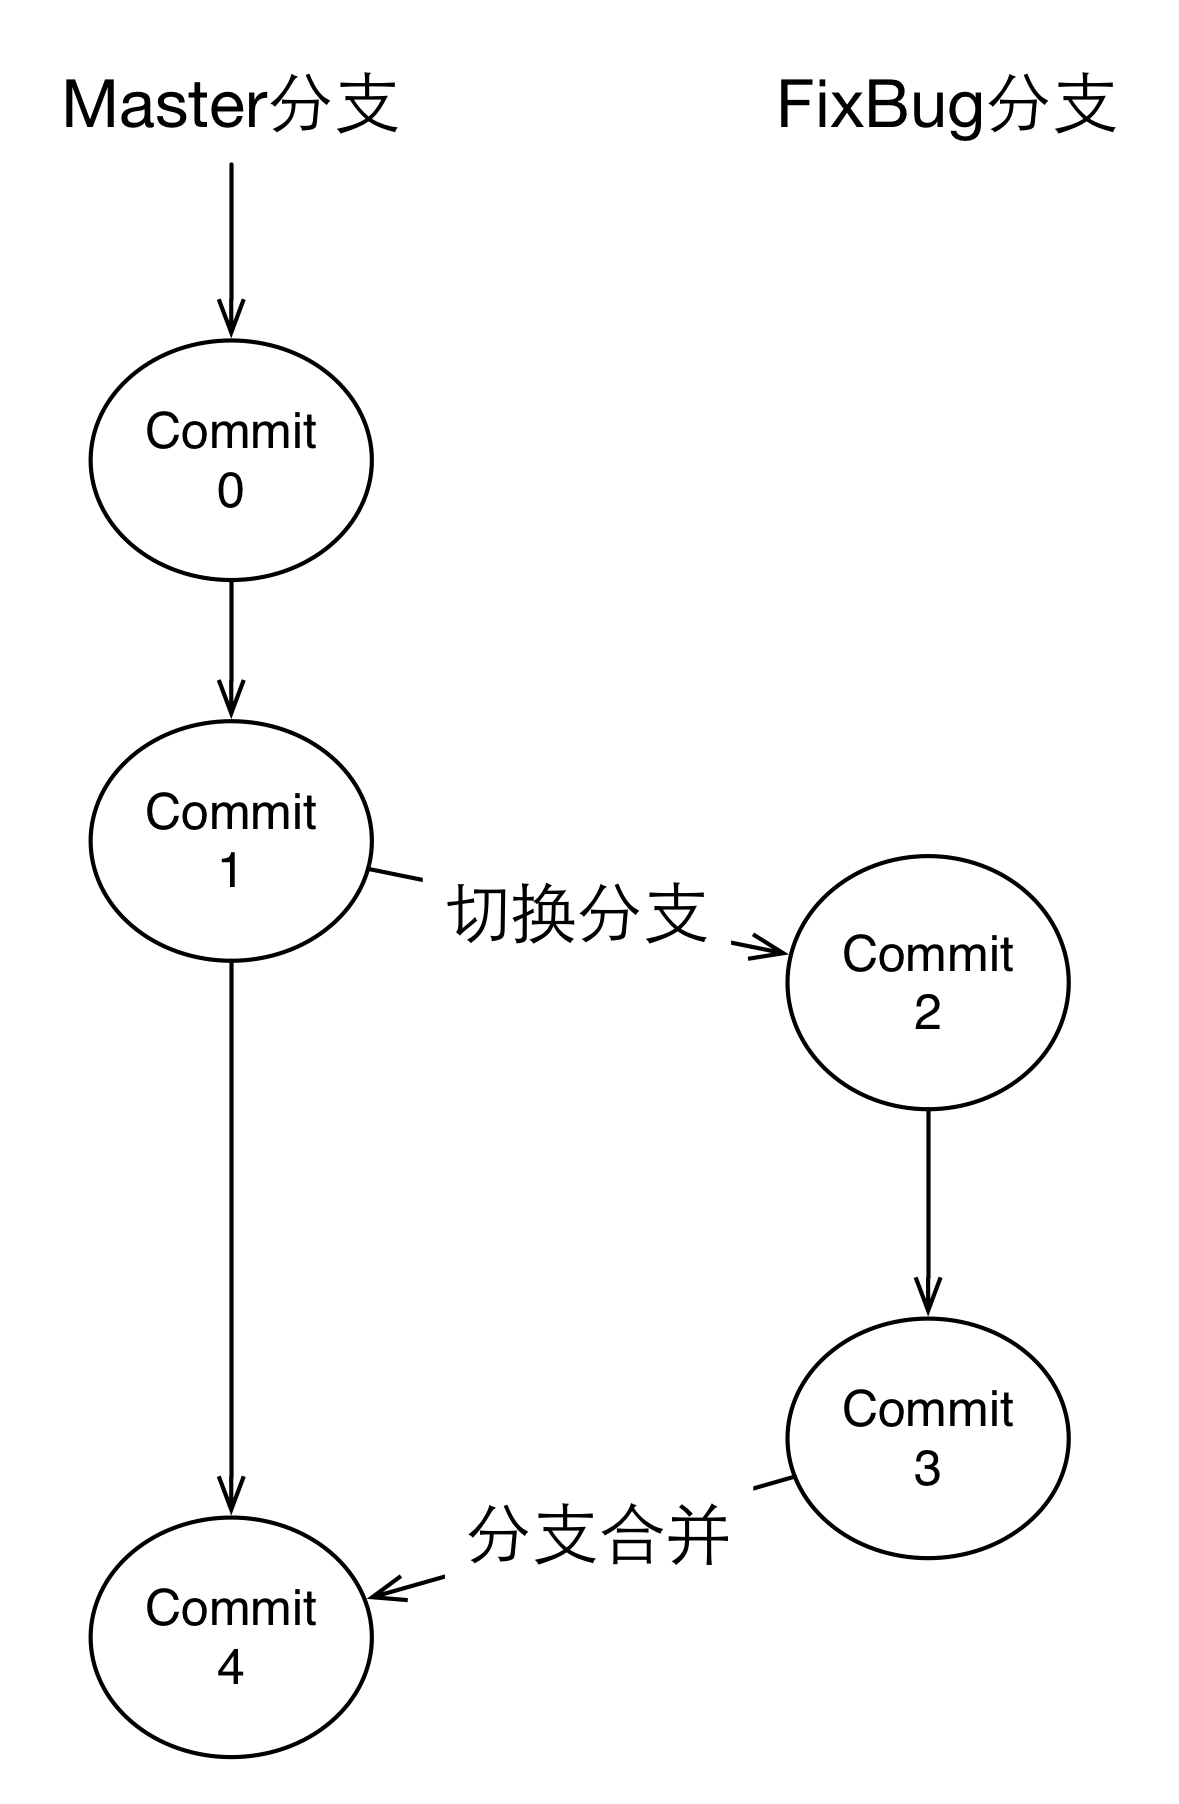
\includegraphics[width=.8\columnwidth]{chap03_git_branch}
	\caption {git分支切换与合并}	
	\label {git_branch}
\end{figure}


\subsection{补丁冲突}
\label {conflict}

可以发现,为了解决问题\ref {origin}的第二点,我们主要需要从代码中挖掘中两类信息:
\begin{enumerate}
	\item 代码的变更集合,即两个版本之间代码的差异性。用于进行问题规约。
	\item 变更的影响集合,即变更集合对代码中其他哪些部分会造成影响。用于确定变更造成的语义影响。
\end{enumerate}

在有了这两类集合之后,我们就可以界定出软件变更在语义层面上对代码的语义影响域,我们可以将这整个过程称为语义影响域分析(Semantic Impacted Area Analysis)。

下面首先给出语义影响域的概念。

\begin{definition}
	程序结构——指程序的基础语法结构,包括类、方法、基本块、语句等不同级别。
\end{definition}

\begin{definition}
	语义影响域(Sematic Impated Area)——在程序的某个限定范围中,直接或间接受到变更影响的程序结构集合。
\end{definition}

可见,语义影响域描述了变更对于程序中其他部分的语义影响。为了更清楚的理解,下面给出影响域的形式化定义。

\begin{definition}
	$impact: Patch \times Code \mapsto \{Structure\}$。$impact(p_m, v_k) = \{ \forall structure_j \subset Struct(v_k) \mid structure_j = im(sturcture_i), \exists change(structure_i) \subset p_m,structure_i,\subset Struct(v_k),v_k \subset Code,p_m \subset Pat(v_k), i,j,k,m \subset \mathbb{N} \}$。该函数用于描述补丁$p_m$对于其所应用的某个版本代码$v_k$的影响域。
\end{definition}

为了挖掘出这两类信息,可以将语义影响域分析划分为两个子过程:
\begin{enumerate}
	\item 程序间差异性分析:获取两个软件版本间的差异性,获得结构化的软件变更信息。该分析过程即为$diff(v_1,v_2)$函数的具体实现。
	\item 变更影响分析:分析软件变更对软件其他部分是否存在影响,并找到受影响的集合。该分析过程即为$impact(p_1,v_1)$函数的具体实现。
\end{enumerate}

我们可以将整个语义影响域分析过程定义为如下的函数:

\begin{definition}
	$ia: Code \times Code \mapsto {Structure}$。$s = ia(v_i,v_j) = impact(diff(v_i,v_j),v_i),i,j \subset \mathbb{N}$。该分析过程先将版本演进的过程转化为补丁,再去计算补丁对程序代码的语义影响域。
\end{definition}

通过语义影响域分析,我们就可以从代码中挖掘出所需要的变更影响信息,从而可以进行后续的分析工作。

事实上,可以将程序中受变更影响的部分划分为不同的粒度,从而获得不同程度的影响,我们考虑对面向对象的编程方法中的影响元素级别进行划分:

\begin{enumerate}
	\item 类:探讨变更对于其他类和对象的影响。对于面向对象的程序设计方法而言,这是最高级别的粒度。
	\item 方法:探讨变更对于其他方法的的影响。
	\item 基本块:探讨变更对于其他基本块的影响。
	\item 语句:探讨变更对于其他语句的影响。
\end{enumerate}

而所谓的影响范围也需要界定其粒度,不同层级的粒度显然会对语义影响域分析的精度产生影响。

\begin{enumerate}
	\item 类间:考虑变更的影响可能延伸到其他类、对象。
	\item 方法间:考虑变更的影响可能延伸到其他方法内部。
	\item 方法内部:考虑变更的影响只在本方法的内部延伸。
\end{enumerate}

在实际情况中,不同级别的影响范围均可分别采用不同的影响元素级别。

在有了软件变更的语义影响域之后,我们可以通过简单地比较两个补丁对代码的影响域是否存在重叠来判定其是否发生了语义冲突。因此可以给出更详细的语义冲突的定义。

\begin{definition}
	\label {define_conflict}
	语义冲突(Semantic Confilict)——指两个补丁所对应的不同变更集合之间存在某两条互斥的变更。
	其中两条变更互斥指二者对同一行代码进行了修改,或者他们所修改了不同行代码,但其影响传播到了某行相同的代码。
\end{definition}

上述定义是对语义冲突的非形式化的描述,为了更清楚的理解,可以给出如下的形式化定义。

\begin{definition}
	\label {problem}
	如果$\exists c_m \subset p_i, \exists c_n \subset p_j$,其中$c_m = change(structure_m),c_n = change(structure_n)$, $structure_m \subset Struct(v_k), structure_n \subset Struct(v_k), v_k \subset Code$,并且$i,j,k,m,n \subset \mathbb{N}$。
	那么有$conflict(p_i,p_j) == true \iff (structure_m == structure_n) \lor (impact(p_i,v_k) \cap impact(p_j,v_k) \neq \varnothing)$,其中$p_i,p_j \subset Pat(v_k)$。
\end{definition}

可见,如果两个补丁对代码的影响域不存在重叠,那么他们两者之间自然是兼容的,因为他们不仅本身的变更互不干涉,并且他们所影响到的程序结构也互不干涉。在这样的情况下,补丁是可以成功应用到其他版本上的代码,并且可以完成补丁本身的目标的。

如果影响域发生了重叠,那么我们就可以认为补丁之间是不相容的,因为补丁所作的变更会对相同的程序结构产生影响。

实际上这样的影响是否能够兼容还需要人工的判定,因为在不同的情况下,他们可能是兼容的,也可能是不兼容的。而我们无法从代码中获取到足够的信息来进行这样的判定,需要人类对于变更的期望信息作为辅助。

我们可以将这个过程定义为如下类型的函数,并称之为冲突分析。可见,我们采用了$isCompatible(s_i,s_j)$函数来作为$conflict(p_i,p_j)$的具体实现。

\begin{definition}
	$isCompatible(s_i,s_j) : 、\{Structure\} \times \{Structure\} \mapsto Boolean$。其中$conflict(p_i,p_j) = isCompatible(impact(p_i,v_i),impact(p_j,v_j)),i,j \subset \mathbb{N}$。
\end{definition}

显然,可以发现,对于问题\ref {origin}的第二点,其核心在于:
\begin{itemize}
	\item 如何规约该问题并计算影响域?即$diff(v_i,v_j)$和即$impact(p_i,v_k)$函数的具体实现。也就是整个语义影响域分析的过程。
	\item 如何判定发生了冲突?即$conflict(p_i,p_j)$函数的实现。也就是整个冲突分析的过程。
\end{itemize}


\section{解决方案}
\label {problem_solve}

考虑前两节中所提到的应用场景和对问题的分析,我们可以给出一个通用的解决方案来解决整个兼容性问题的判定。

\subsection{整体架构}
\label {problem_all}

根据章节\ref {problem_analysis}中的问题分析,实际上整个问题\ref {origin}的解决过程可以参考图\ref {all_flow}。其输入输出的描述参考表\ref {all_io}。

可见,整个解决方案的实现过程包括三个过程:
\begin{itemize}
	\item 补丁应用过程。即$merge$函数的实现过程。
	\item 语义影响域分析过程。即$diff$函数和$impact$函数的实现过程。
	\item 冲突分析过程。即$conflict$函数的实现过程。
\end{itemize}

\begin{figure}[H]
	\centering
	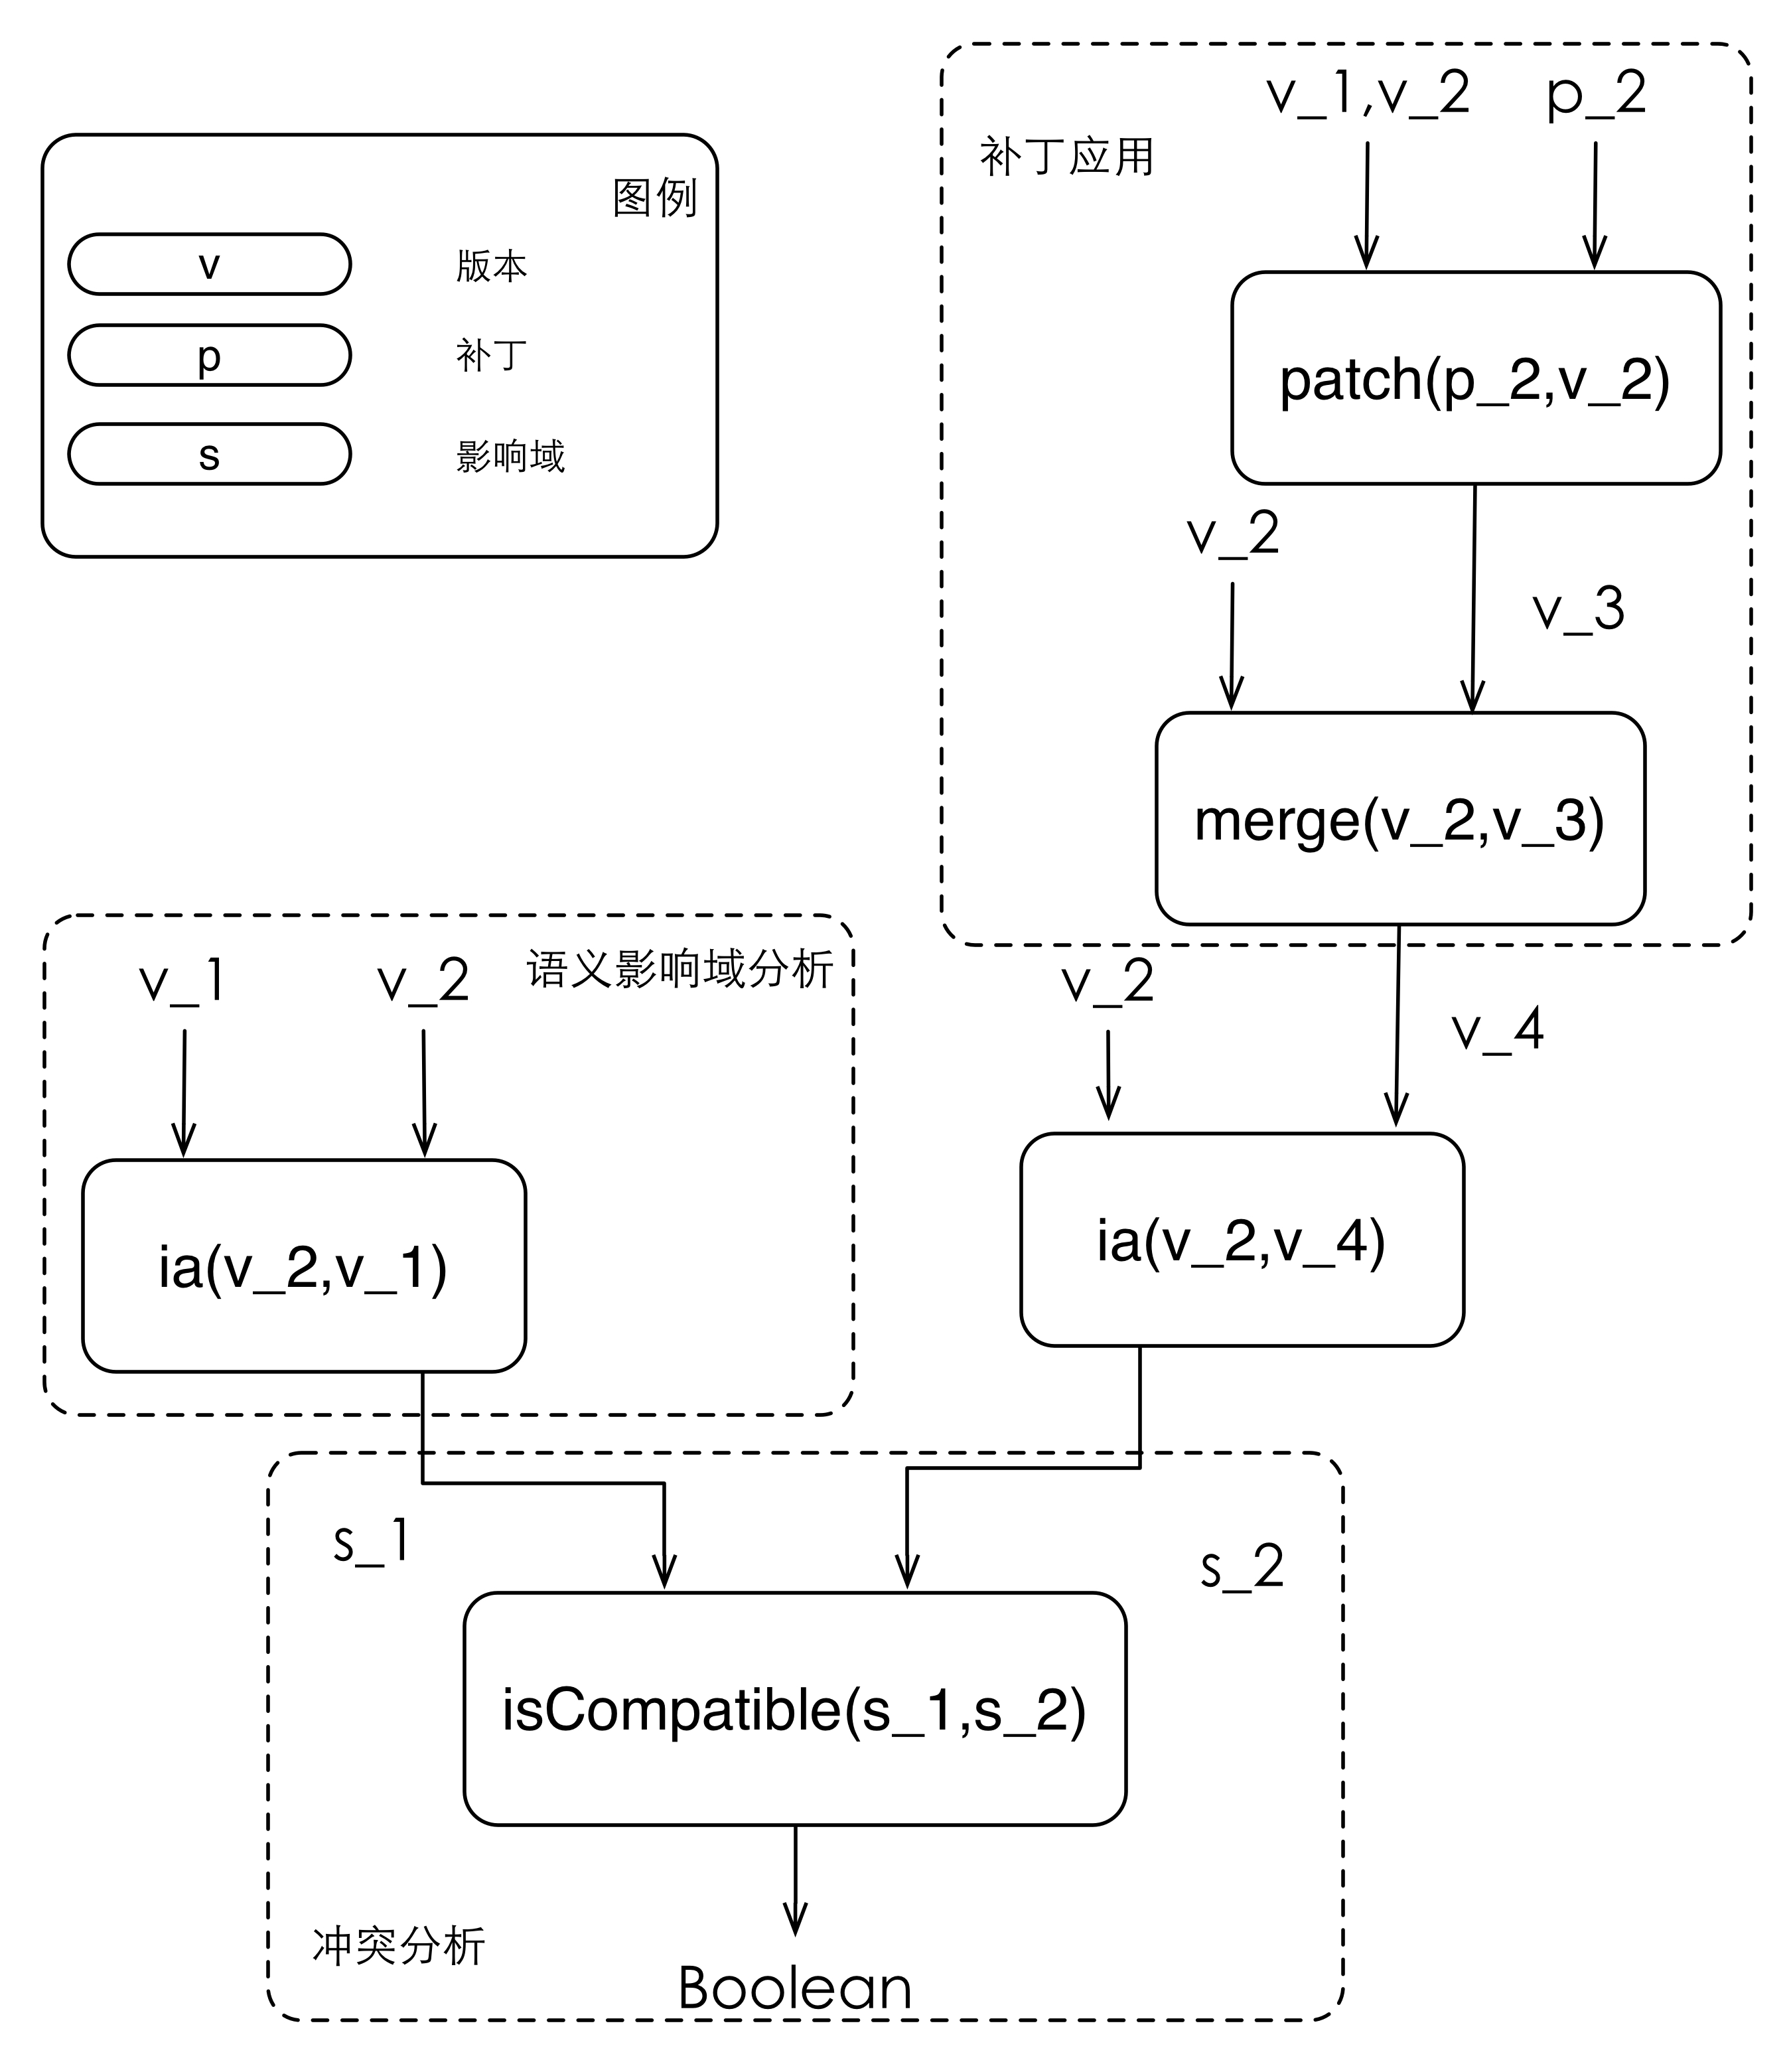
\includegraphics[width=.8\columnwidth]{chap03_all_flow_2}
	\caption {解决方案}
	\label {all_flow}	
\end{figure}

\begin{table}[H]
	\caption{输入输出对照表}
	\label{all_io}
	\centering
	\begin{tabular}{lc}
		\toprule[1.5pt]
		{\heiti 输入输出} & {\heiti 描述}\\\midrule[1pt]
		$v_1$ & 旧版本源代码,待检测的对象 \\
		$v_2$ & 新版本源代码 \\
		$v_3$ & 将补丁$p_2$应用于版本$v_2$后的源代码 \\
		$v_4$ & 将补丁$p_2$中的变更应用于版本$v_1$后的源代码 \\
		$p_2$ & 适用于$v_2$的补丁,待检测的对象 \\
		$s_1$ & $diff(v_2,v_1)$对版本$v_2$的影响域 \\
		$s_2$ & $diff(v_2,v_4)$对版本$v_2$的影响域 \\
		Boolean & 是否冲突 \\
		\bottomrule[1.5pt]
	\end{tabular}
\end{table}

\subsection{补丁应用}

如章节\ref {patch_app}中所述,我们可以采用常见的版本控制工具提供的三路归并算法进行补丁的版本迁移工作。具体来讲,其流程可以简述如下:
\begin{enumerate}
	\item 将补丁$p_1$应用到版本$v_1$,获得旧版本应用补丁后的代码,即其版本为$v_3 = patch(p_1,v_1)$。
	\item 采用三路归并算法实现$v_4 = merge(v_2,v_3)$过程,获得新版本应用补丁后的代码$v_4$。
	\item 解决分支合并中可能出现的冲突问题。
\end{enumerate}

其中,通过三路归并算法进行的合并工作中可能会出现冲突,这说明版本$v_2$和$v_3$之间存在语法冲突,即这两个版本在语法层面上不兼容。我们可以通过人工修改的方式进行修复,实现语法层面上的兼容性。

在解决冲突的过程中可以采用第三方的合并工具,利用现成工具的高效算法快速解决冲突。

该补丁应用的过程主要用于解决补丁的版本适应性问题,整个过程可以用算法\ref {algo_patch}描述如下。

\begin{algorithm}[H]
	\caption{补丁应用}
	\label{algo_patch}
	\begin{algorithmic}[1]
		\Require $v_1,v_2,p_1$
		\Ensure $v_4$
		\State $v_3 \gets patch(p_1,v_1)$
		\State $v_4 \gets merge(v_2,v_3)$
		\State $v_4 \gets resolve(v_4)$
		\State\Return{$v_4$}
		\State
		\Function {merge}{$new,old\_patched$} 
			\State\Return{$3-way-merge(old,new,old_patched)$}
		\EndFunction
		\State
		\Function {resolve}{$version$} 
			\State\Return{$mergetool(version)$}
		\EndFunction		
	\end{algorithmic}
\end{algorithm}

\subsection{语义影响域分析}
\label {sia}

如章节\ref {conflict}中所述,我们需要进行语义影响域分析来获取两个补丁的影响域,用于进行冲突分析使用。

实际上,语义影响域分析主要分为两个分析过程,即程序间差异分析和变更影响分析,通过这两个分析的协作来完成整个语义影响域的分析。

\subsubsection{程序差异性分析}

程序差异性分析是$diff$函数的实现。它主要用于分析两个不同版本的程序间的差异性,其结果即我们所需要的程序变更集合。近年来程序差异性分析方面有不少工作,实现了一些较为成熟的比较工具,我们可以使用这些工具来实现该分析过程。

在本文的组合架构中,程序差异性分析的主要任务是接受两个不同版本的源代码,并返回代码间的结构化差异信息。结构化的差异信息可以视为补丁的一种,只不过它具有比常见的采用Unix diff工具生成的$.patch$类型的补丁文件更丰富的信息,能够描述以程序语法结构的形式对软件变更进行描述。

该分析过程应该满足如下需要:
\begin{itemize}
	\item 输入为两个不同版本的代码。
	\item 输出为源代码间的软件变更集合。
	\item 每条变更描述语句或基本块级别的变更。
	\item 每条变更描述新旧程序结构的相关信息和其关联关系。
	\item 每条变更描述了其所属的作用域。
\end{itemize}

选择这样的分析结果类型是为了后续分析过程的方便,因为变更影响分析需要我们提供软件变更集合作为输入,而$.patch$类型的补丁文件只描述文本行的变更,不包含语法信息,我们无法从中提取出所需的语法层面的变更信息。

一种比较好的选择是采用AST差异性分析,因为抽象语法树中包括了足够多的语法结构信息。



%图中所描述的软件变更集合可以定义如下:
%\begin{definition}
%	$ change\_set = \{ (old_i,new_i) \mid  old_i \subset Structure,new_i \subset Structure, i \subset \mathbb{N} \}$
%\end{definition}



\subsubsection{变更影响分析}

程序变更影响分析是$impact$函数的具体实现。主要用于获取变更集合对其他程序结构的影响域,该集合所包含的程序结构直接或间接地受到变更集合中的元素影响。近年来这方面比较成熟的工作也有不少,因而可以直接选择合适的变更影响分析算法作为该过分析过程的具体实现。

在本文的组合架构中,该分析过程应当接受两个不同版本代码间的变更集合作为输入,并输出变更集合所对应的影响集合,这也就是我们所需要的变更集合的语义影响域。变更影响分析的过程可以通过控制流、数据流等信息分析出变更集合中每条变更对其他程序结构是否存在影响,并进行闭包计算即可。

本文对于该分析过程的要求如下:
\begin{itemize}
	\item 接受两个不同版本代码间的变更集合作为输入。
	\item 计算得到该变更集合所对应的影响集合。
	\item 计算过程中可以指定受影响的范围和元素类型。
	\item 影响集合中的元素按照其不同类型进行分类。
	\item 具有影响追踪系统,将计算影响集合的过程进行记录。方便后续的冲突分析过程进行回溯。
\end{itemize}

其中影响追踪系统可以定义成如下类型的函数。该函数接受一个影响域分析函数$ia(v_i,v_j)$,并返回对应的依赖关系集合。

\begin{definition}
	$impact\_track(ia(v_i,v_j)):(Code \times Code \mapsto {Structure}) \mapsto {depend}$
\end{definition}


%该分析过程如图\ref {impact_analyzer}所述,其中的$impact$函数可以任意选择某一能够满足上述要求的变更影响分析算法。
%
%图中所描述的变更影响集合可以定义如下:
%\begin{definition}
%	$impact\_set = \{ (structure_i) \mid  structure_i \subset Structure, i \subset \mathbb{N}\}$
%\end{definition}
%
%\begin{figure}[H]
%	\centering
%	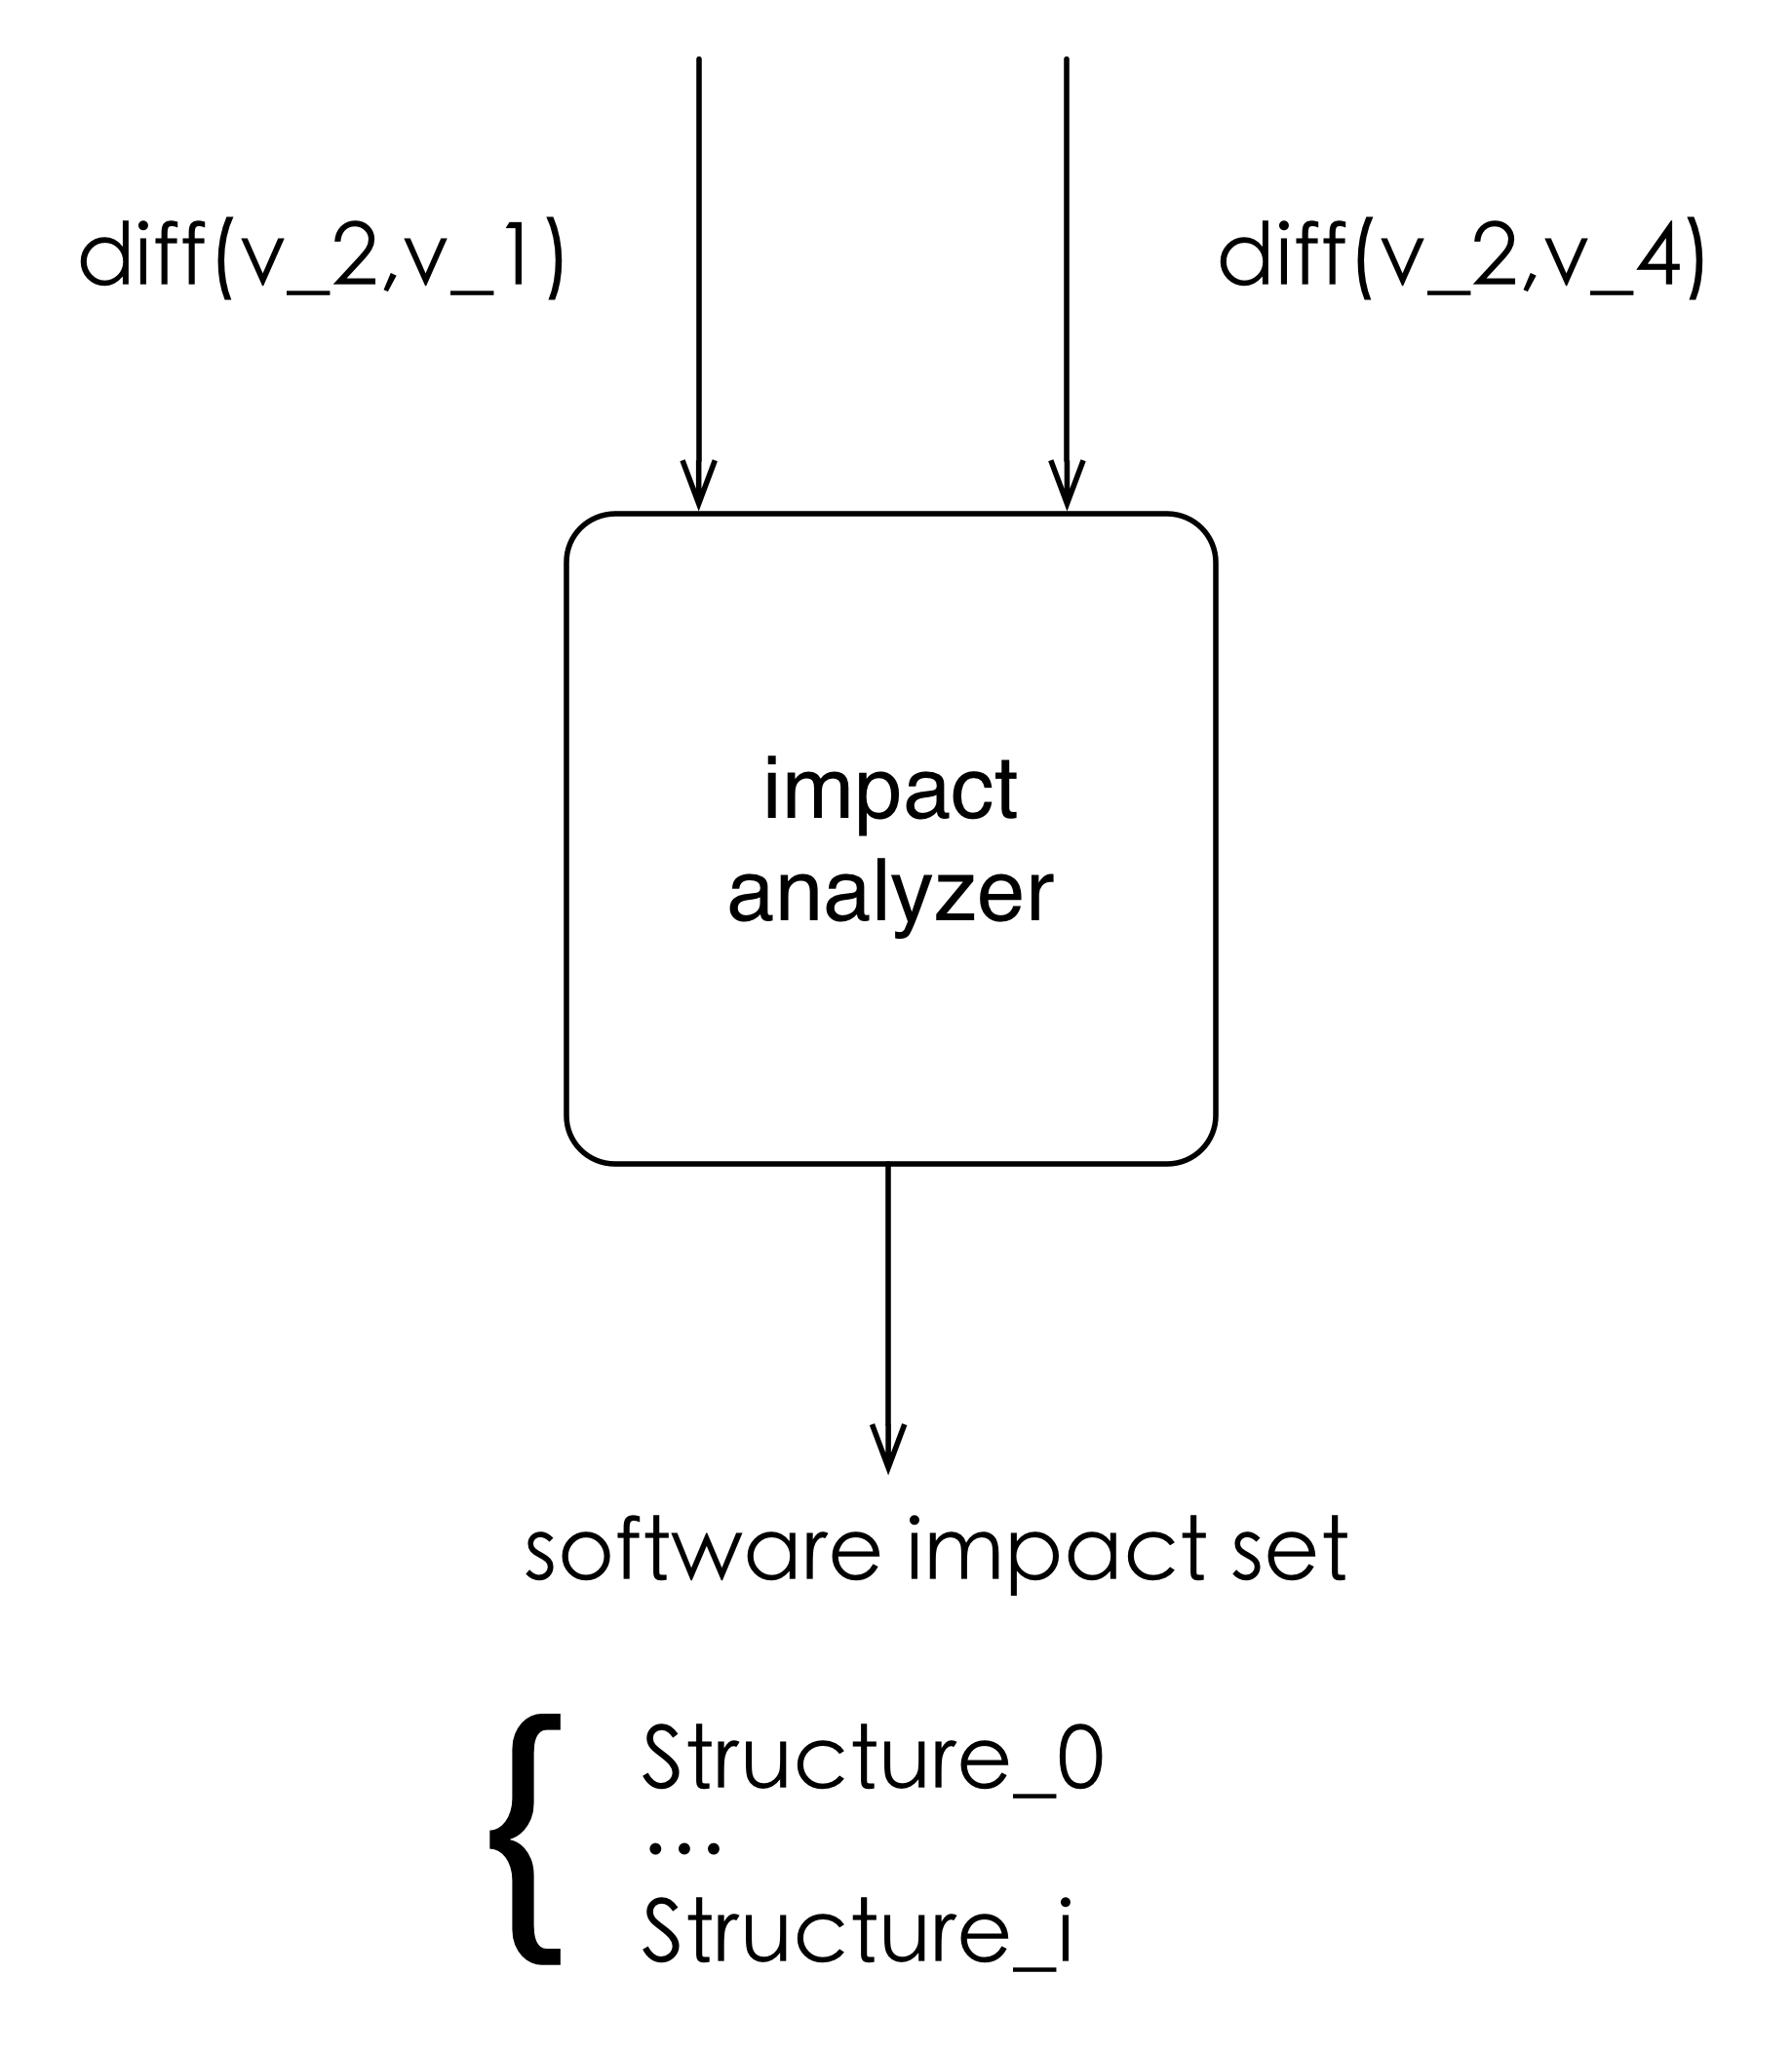
\includegraphics{chap03_impact}
%	\caption {程序间差异分析}
%	\label {impact_analyzer}	
%\end{figure}

在完成了上述两项子分析过程后,我们就完成了整个语义影响域分析过程,并获得了两个不同版本代码的变更集合和对应的其语义影响范围。接下来就可以进行具体的兼容性分析工作。

整个语义影响域分析过程可以用算法\ref {algo_impact}描述。

\begin{algorithm}[H]
	\caption{语义影响域分析算法}
	\label{algo_impact}
	\begin{algorithmic}[1]
		\Require $v_i,v_j$	
		\Ensure $s_i$
		\Function {ia}{$v_i,v_j$}
			\State $p \gets diff(v_i,v_j)$
			\State $s \gets impact(p,v_i)$
			\State\Return{$s_i$}
		\EndFunction
	\end{algorithmic}
\end{algorithm}

\subsection{冲突分析}

冲突分析即为$conflict$函数的具体实现。我们将对比两个版本代码的影响域,确定他们是否重叠,以此为依据判断其兼容性。

理论上来讲,这种简单比对即可发现两个版本间的兼容性问题,因为一旦发生重叠,那么重叠的代码部分显然是会发生兼容性问题的。然而在实际情况中,受限于工具的精度,我们往往不能达到理论上的准确度,而可能会发生误报(False Positive)等情况。

显然,如果重叠不存在,则兼容性是可以得到满足的。而对于如何界定重叠部分的兼容性,则需要人工分析的介入,因为这部分代码的兼容性与补丁的功能目标密切相关,而我们无法从代码中获取到这种信息,因而只有依靠外界来提供,并以此为依据进行详细分析过程,界定这部分代码是否真的存在冲突。

在进行人工分析的过程中,我们不仅需要知道哪部分代码出现了重叠现象,而且还需要知道是哪些变更影响到了这部分代码,因而我们需要引入影响追踪系统来记录变更影响分析过程的轨迹。影响追踪系统可以记录下变更影响分析过程中的每一步,从而获取到程序结构间的影响关系链,事后通过回溯即可追踪到具体的软件变更可见,本过程中主要需要影响追踪系统的回溯模块的支持。

%可以看得出来,由于使用了更严格的冲突定义,我们的方法会造成一定的过高估计的结果。

该分析过程可以参考算法\ref {algo_compatible}。

\begin{algorithm}[H]
	\caption{冲突分析}
	\label{algo_compatible}
	\begin{algorithmic}[1]
		\Require $s_1=ia(v_2,v_1)$,$s_2=ia(v_2,v_4)$\\
				 \quad \quad $t_1=impact\_track(ia(v_2,v_1))$, $t_2=impact\_track(ia(v_2,v_4))$
		\Ensure $isCompatible(diff(v_2,v_1), diff(v_2,v_4))$
		\If{$s_1 = \varnothing \lor s_2 = \varnothing$}
			\State $result \gets True$
		\Else
			\State $s \gets s_1 \cap s_2$
			\If{$s = \varnothing$}
				\State $result \gets True$
			\Else				
				\State $result \gets Manual\_analysis(s_1, s_2, t_1, t_2)$
			\EndIf 
		\EndIf
		\Return $result$
	\end{algorithmic}
\end{algorithm}

%整个分析过程的架构如图\ref {isCompatible}所示。
%
%\begin{figure}
%	\centering
%	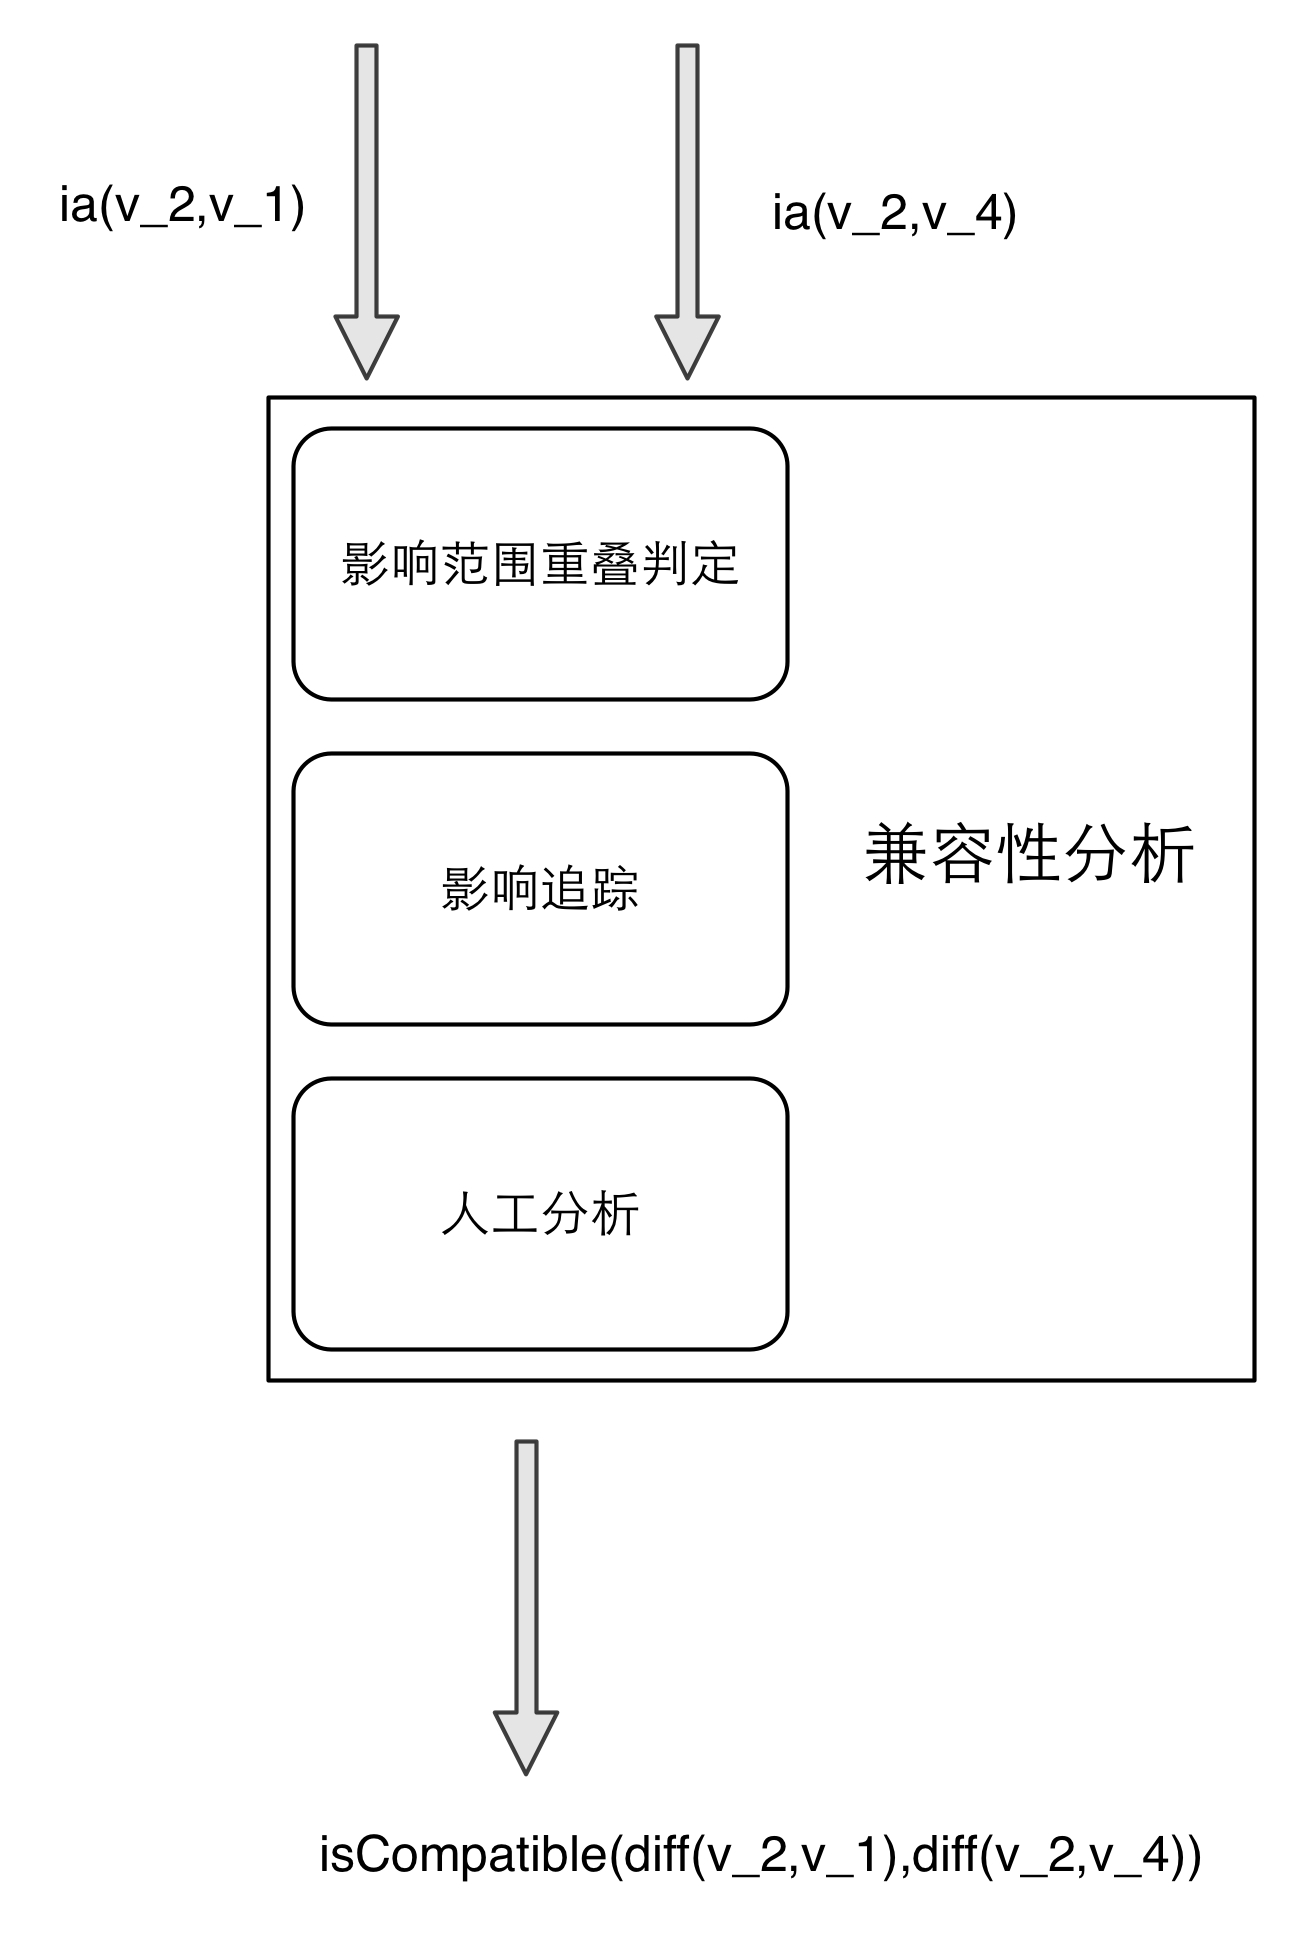
\includegraphics{chap03_isCompatible}
%	\caption {兼容性分析}
%	\label {isCompatible}	
%\end{figure}


\section{本章小结}
本章主要介绍了软件补丁兼容性检测所关注的主要问题以及如何解决该问题。

章节\ref {define_problem}介绍了问题定义。

章节\ref {problem_analysis}中对问题进行了深入分析和讨论,提出了解决该问题所需要做的分析工作。

章节\ref {problem_solve}介绍了如何将前一节中提到的分析方法进行整合,形成一套通用解决方案,同时还对其中每个分析方法所需要遵守的约定和算法进行了描述。
\chapter{方法实现}
介绍如何将版本管理、程序间差异分析、变更影响分析、兼容性分析算法组合成整体的流程。
%\chapter{软件变更影响域分析}
\label{chap_impact}

本章中主要介绍软件变更影响域分析的相关概念、分析方法和工具模块的设计与实现。

如前所述,我们需要对补丁中的变更进行变更影响域分析,以此来找到变更对应的语义影响域,即所谓的变更影响域,用于进行后续的冲突检测。

软件变更是对程序代码结构所作出的修改,它会将原有的代码结构变更为新的代码结构。因此,由于修改前的代码结构与软件中其他代码结构的耦合性,在应用软件变更之后,会导致这些相关的代码结构的行为受到该软件变更的影响,具体是什么影响则需要根据变更的语义来判断。

我们将这些受到补丁中变更影响的代码结构集合称之为变更影响域。其更详细的定义可以参考后续的相关定义。


为了找到所谓的变更影响域,我们需要从代码中挖掘中两类信息:
\begin{enumerate}
	\item 代码的变更集合,即两个版本之间代码的语法差异性。用于寻找变更的影响域。
	\item 变更的影响域,即受变更集合的语义影响的其他程序语法结构。用于确定变更造成的语义影响。
\end{enumerate}

在有了这两类集合之后,我们就知道了软件变更对代码的语义影响域,我们可以将这整个过程称为变更影响域分析。

可见,软件变更影响域分析的过程也就是找到软件变更,并分析得到变更影响域的过程。这些找到的变更影响域将作为软件变更冲突检测过程中的输入,用于判断变更影响域之间是否会产生冲突。

因此,该过程可以分为两个步骤。首先,变更影响域分析需要找到不同版本代码之间的软件变更集合。其次,变更影响域分析会根据找到的软件变更集合,分析并得到变更影响域。

如上所述,那么软件变更影响域的过程也就可以相应地拆分为两个子分析过程。首先,使用程序间语法差异性分析来完成寻找软件变更集合的过程,其次,使用变更语义影响分析来完成寻找变更影响域的过程。

因此,该过程所对应的影响域分析模块在实现的过程中也将对应地拆分为两个子模块:
\begin{enumerate}
	\item 差异性分析模块。该模块将实现程序间语法差异性分析的过程。
	\item 影响分析模块。该模块将实现变更语义影响分析的过程。
\end{enumerate}

由于这两个子分析过程已经有许多相关的工作出现,因此我们在实现检测工具中对应的影响域分析模块的时候将采用已有的成熟算法来完成。工具实现的主要精力将放在子模块的整合和调整过程上。

下面将分别对这两个分析过程和其模块设计与实现进行介绍。


%通过语义影响域分析,我们就可以从代码中挖掘出所需要的变更影响域信息,从而可以进行后续的冲突检测工作。
%
%实际上,语义影响域分析主要分为两个子过程,即程序间差异分析和变更语义影响分析,通过这两个分析的协作来完成整个语义影响域的分析。
%
%我们可以将整个语义影响域分析过程定义为如下的函数,该分析过程先将版本演进的过程转化为补丁,再去计算补丁对程序代码的语义影响域:
%
%\begin{definition}
%	$ia: Code \times Code \mapsto {Structure}$。$s = ia(v_i,v_j) = impact(diff(v_i,v_j),v_i),i,j \subset \mathbb{N}$。
%\end{definition}
%
%因此,整个语义影响域分析过程可以用算法\ref {algo_impact}描述。
%
%在兼容性检测工具中,该部分工作被实现为影响域分析模块,该模块需要对$ia$函数进行实际的实现。因此,该模块可以对应地拆分为两个子模块分别进行实现:
%\begin{itemize}
%	\item 差异性分析模块:实现相应的程序差异性分析过程。即$diff$函数的实现。
%	\item 影响分析模块:实现相应的变更语义影响分析过程。即$impact$函数的实现。
%\end{itemize}
%
%该模块中首先需要定义好合适的影响范围和影响元素的级别。
%
%事实上,可以将程序中受变更影响的部分划分为不同的粒度,从而获得不同程度的影响\cite{petrenko2009variable},我们考虑对面向对象的编程方法中的影响元素级别进行划分:
%
%\begin{enumerate}
%	\item 类:探讨变更对于其他类和对象的影响。对于面向对象的程序设计方法而言,这是最高级别的粒度。
%	\item 方法:探讨变更对于其他方法的的影响。
%	\item 基本块:探讨变更对于其他基本块的影响。
%	\item 语句:探讨变更对于其他语句的影响。
%\end{enumerate}
%
%而所谓的影响范围也需要界定其粒度,不同层级的粒度显然会对语义影响域分析的精度产生影响。
%
%\begin{enumerate}
%	\item 类间:考虑变更的影响可能延伸到其他类、对象。
%	\item 方法间:考虑变更的影响可能延伸到其他方法内部。
%	\item 方法内部:考虑变更的影响只在本方法的内部延伸。
%\end{enumerate}
%
%不同级别的影响范围均可分别采用不同的影响元素级别。
%
%在实际情况中,我们主要采用了较为简单的分析过程,即将影响范围限制在方法内部,但是将受影响元素设置为程序语句级别,以保证精度。
%
%在实现该模块的过程中,由于我们可以采用现有工具来完成具体的程序间差异分析和变更语义影响分析过程,因而这两个子过程的分析算法可以直接使用已有的成熟算法。我们可以将主要精力放在如何整合两个子过程,并将其工具实现进行改进,以适用于兼容性检测问题的具体情况。
%
%下面分别对这两个子过程的分析方法和对应模块的设计与实现进行叙述。
%
%\begin{algorithm}[H]
%	\caption{语义影响域分析算法}
%	\label{algo_impact}
%	\begin{algorithmic}[1]
%		\Require $v_i$,$v_j$,即两个不同版本的代码	
%		\Ensure $s$,即版本间的变更对于版本$v_i$的语义影响域
%		\Function {ia}{$v_i,v_j$}
%		\State $p \gets diff(v_i,v_j)$
%		\State $s \gets impact(p,v_i)$
%		\State\Return{$s$}
%		\EndFunction
%	\end{algorithmic}
%\end{algorithm}

\section{程序间语法差异性分析}
\label {chap_diff}

如前所述,程序间语法差异性分析主要用于完成寻找不同版本间的软件变更的过程,该过程中需要分析代码间的语法结构的差异性,并得出相应的变更集合。可见,在该过程中,我们主要关注程序间的语法结构差异性。


%程序间差异性分析是$diff$函数的实现。它主要用于分析两个不同版本的程序之间的差异性,其结果即我们所需要的程序变更集合。
%
近年来程序间语法差异性分析方面有不少工作,实现了一些较为成熟的比较工具,我们可以使用这些工具来实现其所对应的差异性分析子模块。

\subsection{相关定义}

本节中主要介绍程序间语法差异性分析过程中所涉及到的相关概念的定义,以便能够更清楚的了解该分析过程的实质。

$\mathcal{C}$是某个版本的源代码文件中按照该语言的合法语法结构组织起来的代码(如抽象语法树的形式),即由该语言的相应$\mathcal{S}$组成的集合。$\mathcal{S}$是某种语言的合法语法结构,例如Java语言中的语句、方法定义、类定义等,由于随不同语言的实际情况而变化,在这里不做更具体的定义。$v_k$表示第k个版本的代码$\mathcal{C}$,其中$k \subset \mathbb{N}$。

\begin{definition}
	$\mathcal{P}: S \times S$。$\mathcal{P}$是补丁,也就是变更集合,即一个由$\mathcal{S}$的二元组构成的集合。$\forall c \subset \mathcal{P}$,有$c = (s_i,s_j)$,其中$s_i,s_j \subset \mathcal{S},i,j \subset \mathbb{N}$,$s_i$和$s_j$分别表示变更前和变更后的代码语法结构。
\end{definition}

\begin{definition}
	\label {define_diff}
	$diff : \mathcal{C} \times \mathcal{C} \mapsto \mathcal{P}$。该函数用于求解两个不同版本的代码$v_i$和$v_j$之间的语法差异性,其结果即为变更集合$\mathcal{P}$。
\end{definition}

$diff$函数描述了什么是程序间语法差异性分析,它能够接受两个不同版本的代码,并返回代码间的语法结构差异,也就是该分析所要求的变更集合。

\subsection{分析方法}

在本文的兼容性检测方法中,程序间语法差异性分析的主要任务是接受两个不同版本的源代码,并返回代码间的语法结构上的差异信息。这种结构化的差异信息可以视为补丁的一种,只不过它和常见的采用Unix diff工具生成的$.patch$类型的补丁文件相比具有更丰富的信息,能够以该语言的合法语法结构的形式对软件变更进行描述。

根据上一节中的相关定义,该分析过程应该满足如下需要:
\begin{itemize}
	\item 输入为两个不同版本的源代码。
	\item 输出为源代码间的软件变更集合。
	\item 每条变更描述对于该语言的合法语法结构的变更。
\end{itemize}

除此以外,该分析过程还应当描述的信息包括:
\begin{itemize}
	\item 每条变更描述变更前后语法结构的相关信息,例如该语法结构的位置信息等。让我们能够知道该变更的作用位置等。
	\item 每条变更描述了其所属的作用域。即描述了这些语法结构之间的从属关系,让我们能够知道该变更的作用范围。
\end{itemize}

选择这样的分析结果类型是为了后续分析过程的方便。由于后续的变更语义影响分析需要我们提供软件变更集合作为输入,而$.patch$类型的补丁文件只描述单纯的文本行的变更,不包含语法信息,我们无法从中提取出所需的语法层面的变更信息,因此该类型的差异性分析方法是无法满足我们的需求的。

在实践过程中,一种比较好的选择是在抽象语法树AST(Abstract Syntax Tree)上进行差异性分析,因为抽象语法树中包括了足够的语法结构的相关信息。

\subsection{模块设计与实现}

本文中差异性分析模块在实现中采用了jpf-regression工具自带的前置工具ASTro来进行程序间语法差异性分析过程。该子模块实现了$diff$函数的实际功能,能接受两个不同版本的Java源代码文件作为输入,并以AST的形式输出变更集合。

%\subsubsection{设计}
%
%在该模块的设计中,其输入输出过程可以描述如图\ref {differ},输入输出的具体描述参见表\ref {differ_io}。
%
%\begin{figure}[H]
%	\centering
%	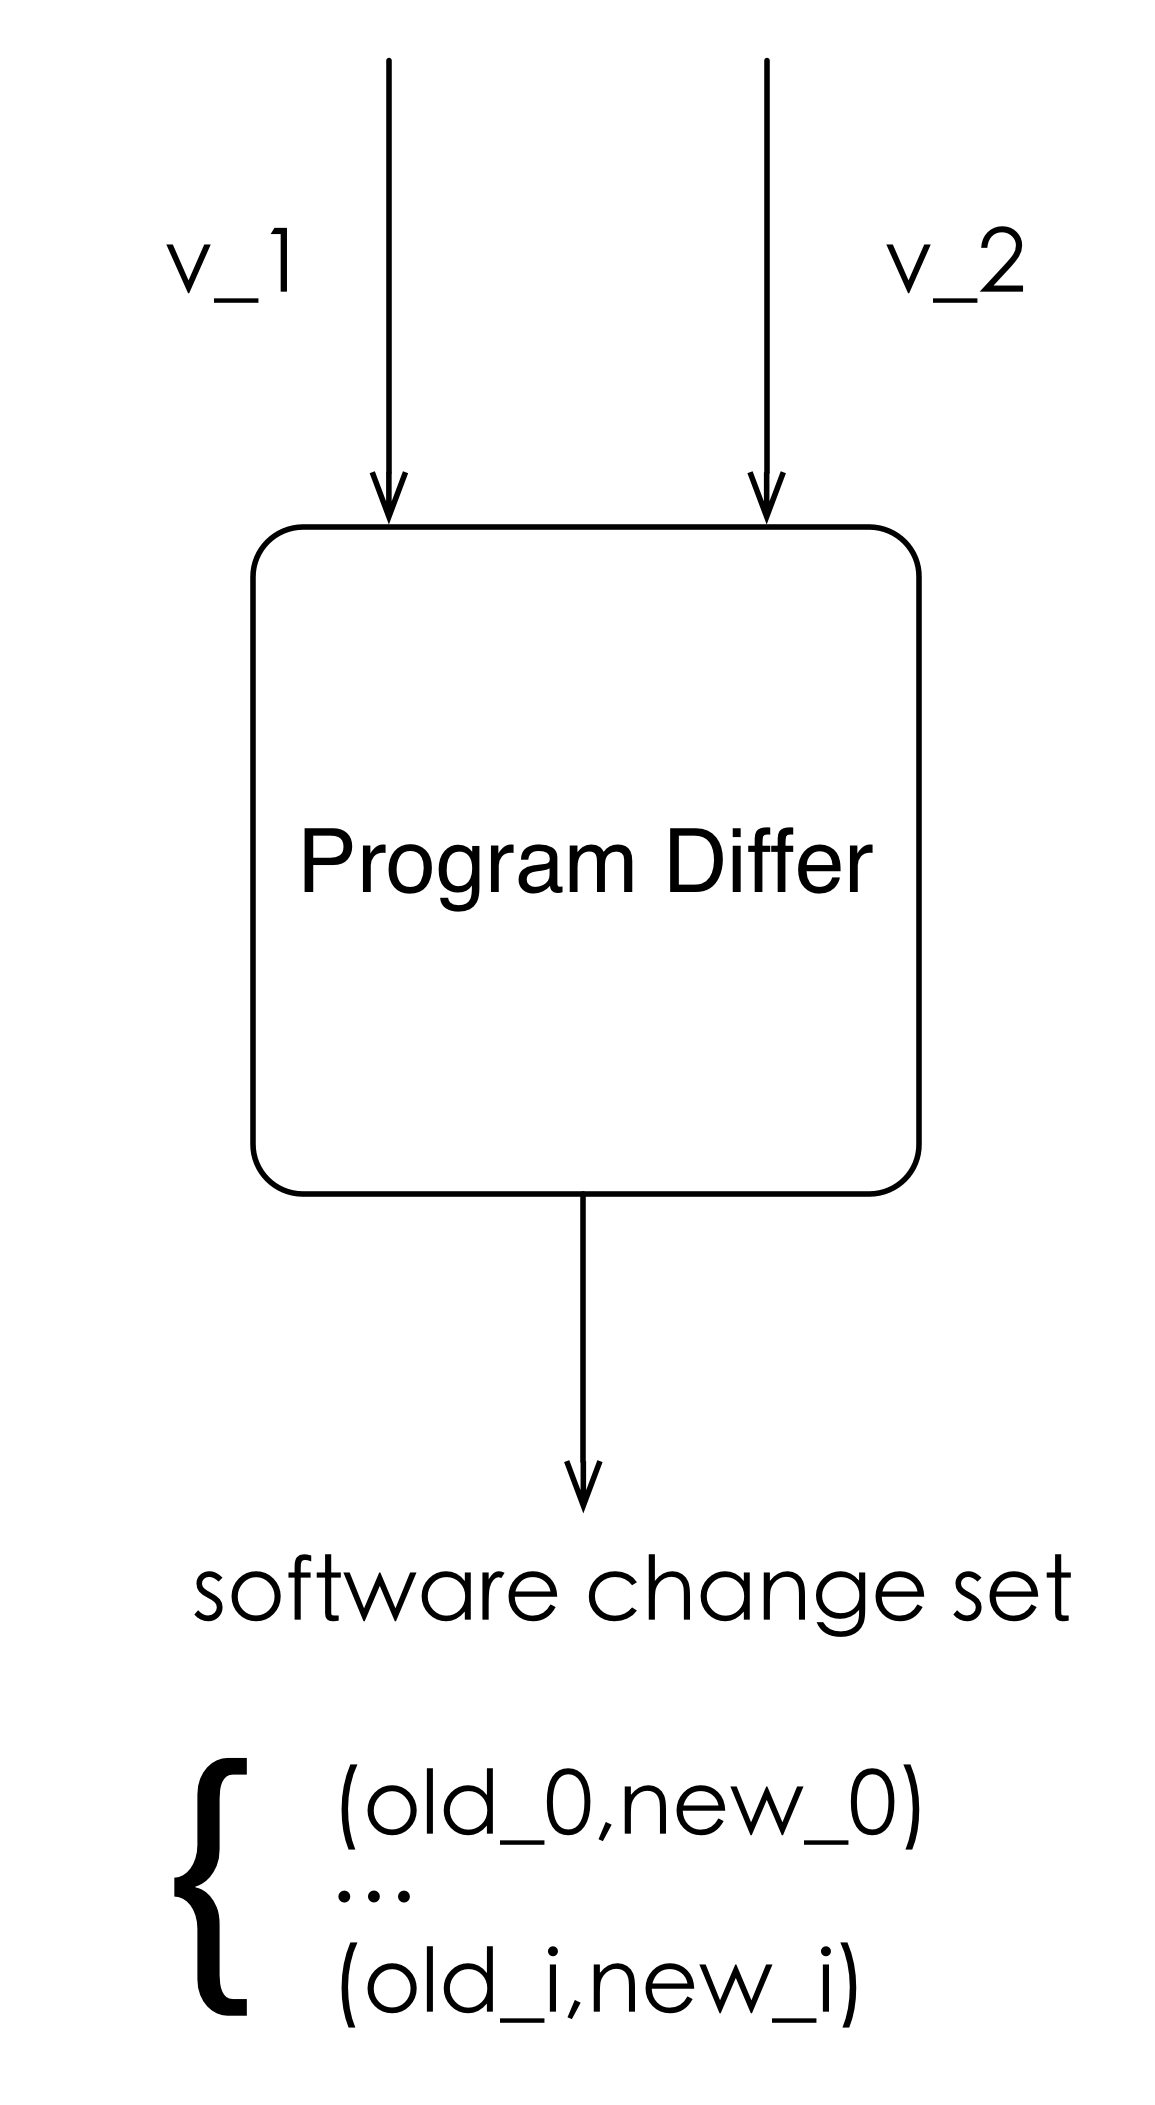
\includegraphics[height=.6\columnwidth]{chap03_differ}
%	\caption {差异性分析模块}
%	\label {differ}	
%\end{figure}
%
%图中所描述的模块输出——软件变更集合,设计为如下的格式,即变更前后的代码结构所组成的二元组集合:
%\begin{definition}
%	$ change\_set = \{ (old_i,new_i) \mid  old_i \subset Structure,new_i \subset Structure, i \subset \mathbb{N} \}$
%\end{definition}
%
%由于该模块需要调用其他工具来完成具体的差异性分析过程,其输出应作为影响分析模块的输入,可见该模块的核心任务包括:
%\begin{itemize}
%	\item 差异性分析
%	\item 输入输出
%\end{itemize}
%
%因此该模块的内部设计可以参考图\ref {des_diff}。
%
%该模块的流程也就可以设计成如下的形式:
%\begin{enumerate}
%	\item 读取输入
%	\item 进行差异性分析
%	\item 输出分析结果
%\end{enumerate}
%
%\begin{figure}[H]
%	\centering
%	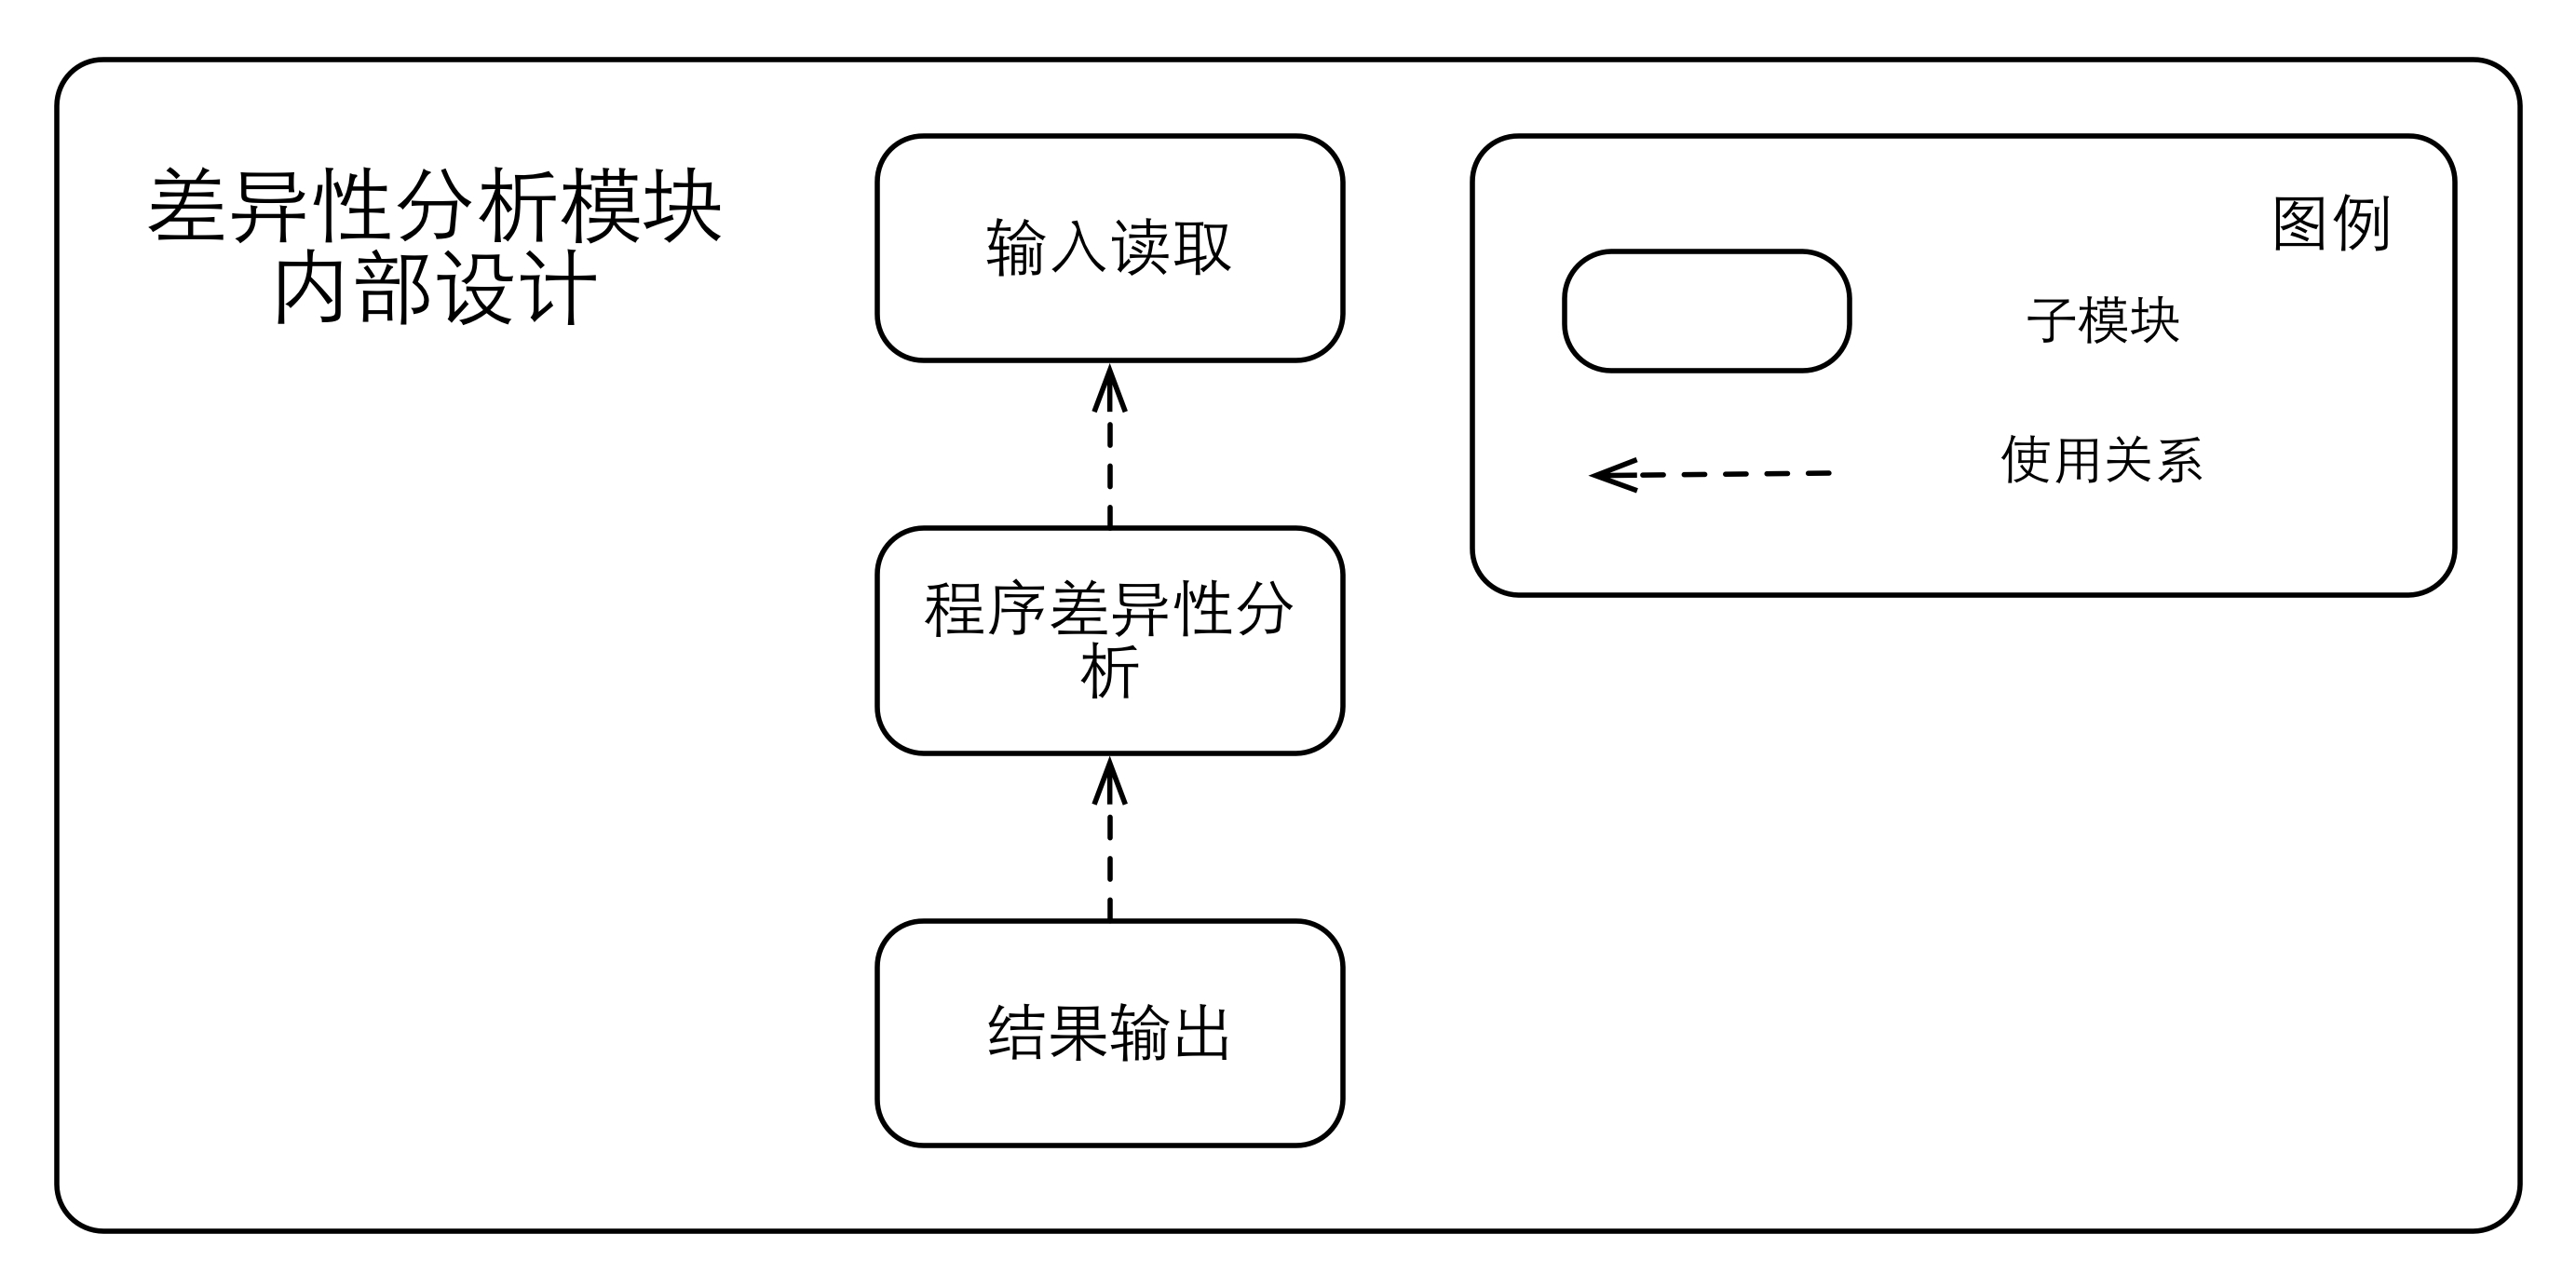
\includegraphics[width=.8\columnwidth]{chap04_diff_des}
%	\caption {模块设计}
%	\label {des_diff}	
%\end{figure}
%
%
%\begin{table}
%	\caption{输入输出对照表}
%	\label{differ_io}
%	\centering
%	\begin{tabular}{lc}
%		\toprule[1.5pt]
%		{\heiti 输入输出} & {\heiti 描述}\\\midrule[1pt]
%		$v_1$ & 源代码 \\
%		$v_2$ & 源代码 \\
%		$change\_set$ & 变更集合 \\
%		\bottomrule[1.5pt]
%	\end{tabular}
%\end{table}
%
%\subsubsection{实现}
%
%在该模块的实现过程中,采用了ASTro工具来完成具体的程序间差异分析过程。
%
%因而实际上该模块的输入输出可以参考表\ref {differ_io2}。
%
%\begin{table}[H]
%	\caption{输入输出对照表}
%	\label{differ_io2}
%	\centering
%	\begin{tabular}{llc}
%		\toprule[1.5pt]
%		{\heiti 输入输出} & {\heiti 描述} & {\heiti 格式}\\\midrule[1pt]
%		输入 & 源代码 & Java\\
%		输入 & 源代码 & Java\\
%		输出 & 影响分析模块配置文件 & JPF\\
%		输出 & 变更集合 & XML\\
%		\bottomrule[1.5pt]
%	\end{tabular}
%\end{table}

ASTro工具支持对Java代码的比对。它会比对两个文件的抽象语法树,并从中抽取出对应的不同之处,形成语法结构上的差异性,并将变更前后的AST输出,为后续的分析过程提供了所需的变更集合。

该工具将源代码按照抽象语法树的格式进行输出,其最小节点级别为基本块,并提供了丰富的差异性信息,例如两个版本的代码间其对应节点是否发生了变更等,其输出格式为XML结构化文档。利用这些输出信息,我们可以从中提取出需要的程序变更集合,从而进行后续的变更语义影响分析。

在实际使用中,为了满足本文的需要,在将该工具整合进来时进行了一些改进。下面将分别进行阐述。

首先,受限于ASTro工具的具体实现,其输出结果存在着一定的问题,因此我们对ASTro工具的输出结果进行了一定的过滤。其输出结果的问题主要包括:
\begin{enumerate}
	\item 对某些代码文件无法完成差异性分析。这可能是由于有的代码文件过于复杂,超出了其工具的分析能力。
	\item 对某些代码文件输出结果不准确,存在误报(False Positive)的问题。这可能是受限于工具中的差异性分析算法的精度,导致将并没有发生变更的语法结构也认为是发生了变更,并进行了分析和输出。
\end{enumerate}

对于第一个问题,由于无法知道该工具的源代码,我们无法解决,不过在实践过程中这只是极少数现象。

对于第二个问题,我们分析其结果可以发现,其结果中存在着误报的情况,即某些代码行并未发生变更,然而工具却报告其发生了诸如移动、先删后增之类的伪变更。同样由于无法知道该工具的源代码,我们无法从算法的角度进行修改,不过对于这样的情况,我们可以对其输出结果进行处理,将这些误报的情况进行过滤,保留一个真变更子集合即可。

该过滤算法可以用伪代码\ref {xml}进行描述。

\begin{algorithm}
	\caption{XML结果过滤算法}
	\label{xml}
	\begin{algorithmic}[1]
		\Require $c_1 = diff(v_2, v_1), c_2 = diff(v_2,v_4)$
		\Ensure 过滤掉两个变更集合中的相同变更
		\State $del_1 \gets \varnothing$
		\State $del_2 \gets \varnothing$
		\For {$i = 0$ to $sizeof(c_1)$}
		\State $tc_1 \gets c_1[i]$
		\For {$j = 0$ to $sizeof(c_2)$}
		\State $tc_2 \gets c_2[j]$
		\If {$tc_1 == tc_2$}
		\State $del_1.add(tc_1)$
		\State $del_2.add(tc_2)$
		\EndIf	
		\EndFor
		\EndFor
		\State $c_1 \gets c_1.delete(del_1)$
		\State $c_2 \gets c_2.delete(del_2)$
	\end{algorithmic}
\end{algorithm}

我们可以归纳证明这种过滤操作的正确性。由于变更对于代码的影响是直接或间接的,对于某次变更语义影响分析的结果$s$而言,假设对于其中任意一个受影响的元素$e_k$,其中$k \subset \mathbb{N}$,其影响来源可能包括如下几种可能:
\begin{enumerate}
	\item 其影响仅来源于变更$c_1$。
	\begin{itemize}
		\item 如果$c_1$为真变更,那么删除所有伪变更对于$e_k$没有影响。
		\item 如果$c_2$为伪变更,那么删除所有伪变更会导致$e_k$从集合s中被删除,但此时$e_k$本身即为伪影响,集合$s$的正确性会得到提高。
	\end{itemize}
	\item 其影响来源于多条变更$c_1,c_2\dots,c_m$,其中$m \subset \mathbb{N}$。
	\begin{itemize}
		\item 假若所有变更均为真变更,那么删除所有伪变更对于$e_k$没有影响。
		\item 假若来源变更集合中包括某几条伪变更,那么删除所有伪变更之后,仍然存在其他真变更,这些真变更仍然会在变更语义影响分析中导致$e_k$被添加到集合$s$中,因而也不会使集合$s$的正确性下降。
		\item 假若所有变更均为伪变更,那么删除所有伪变更会导致$e_k$从集合$s$中被删除,但此时$e_k$本身即为伪影响,集合$s$的正确性会得到提高。
	\end{itemize}
\end{enumerate}

可见,我们的预处理操作是正确的,它不会导致后续的变更语义影响分析结果$s$的正确性降低。

其次,我们完成了分析过程的自动化。

在实现该模块的时候,我们采用了shell脚本来完成分析过程的自动化,使该模块能够循环地调用ASTro进行分析,从而实现对整个软件系统的所有代码文件进行批量化处理。若需要修改该模块的输入信息,只需要修改脚本中对应的输入即可。在这部分工作中,脚本代码主要完成了以下任务:

\begin{itemize}
	\item 输入数据定位,包括Java源代码和编译后的Class文件等。
	\item 根据代码的存放路径,计算其对应Class文件的位置。
	\item 获取代码文件名,以确定本次分析的对象。
	\item 实验数据的依赖JAR包定位。
	\item 创建输出文件目录。
	\item 定义ASTro的输入参数,包括输入文件位置、输出文件位置、查找路径等。
	\item 调用ASTro进行单次分析。
\end{itemize}

其中ASTro工具的使用格式可参考如下,其具体各参数的定义参考表\ref {ASTro}。

\begin{lstlisting} [style=BashInputStyle]
ASTDiffer 3/27/2013
USAGE: java ASTDiffer -original <file>.java -modified <file>.java 
-dir <output folder>
OPTIONAL: -file <fileName> -ocp <classpath> -mcp <classpath> 
-oco <outputDir> -mco <outputDir> -cs -xml
\end{lstlisting}	

\begin{table}[H]
	\caption{ASTro参数对照表}
	\label{ASTro}
	\centering
	\begin{tabular}{llc}
		\toprule[1.5pt] 
		{\heiti 参数名} & {\heiti 描述} & {\heiti 启用}\\\midrule[1pt]
		-file & 分析目标的名字 & 是 \\
		-dir & 输出路径 & 是 \\
		-ocp & 旧版本代码的Classpath & 是\\
		-mcp & 旧版本代码的Classpath & 是\\
		-original    & 旧版本代码的位置 & 是\\
		-modified   & 新版本代码的位置 & 是\\
		-xml   & 以XML格式输出结果 & 是\\
		-cs   & 以变更脚本(Change Script)格式输出结果 & 否\\
		-heu   & 以启发式的方式进行匹配 & 是\\
		\bottomrule[1.5pt]
	\end{tabular}	
\end{table}

而且,我们还采用了shell脚本完成对后续分析过程的支持,使其能够自动批量化创建影响分析模块所需的配置文件。配置文件为自定义的JPF格式,通过类似键值对的方式定义了各项属性的值,可以参考表\ref {JPF_prop}所述。

\begin{table}
	\caption{JPF属性对照表}
	\label{JPF_prop}
	\centering
	\begin{tabular*}{\linewidth}{lp{10cm}}
		\toprule[1.5pt]
		{\heiti 属性名} & {\heiti 描述} \\\midrule[1pt]
		target & 分析的目标 \\
		sourcepath & 源代码路径\\
		rse.ASTResults & ASTro工具的输出文件位置\\
		rse.newClass & 新版本代码的Class文件位置\\
		rse.oldClass    & 旧版本代码的Class文件位置\\
		rse.dotFile   & jpf-regression工具的Dot格式输出文件位置\\
		\bottomrule[1.5pt]
	\end{tabular*}
\end{table}

在使用shell脚本调用ASTro工具进行分析和输出影响分析模块的配置文件时,考虑到实际使用中,我们需要将新版本$v_2$作为对比的基准,以获取一致的行号。因而在进行变更语义影响分析时,我们需要进行相应配置,使得:
%\begin{itemize}
%	\item $s_1 = impact(diff(v_2,v_1),v_2)$,求得变更集合$p_1 = diff(v_2,v_1)$对版本$v_2$的影响范围$s_1$。
%	\item $s_2 = impact(diff(v_2,v_4),v_2)$,求得变更集合$p_3 = diff(v_2,v_4)$对版本$v_2$的影响范围$s_2$。
%\end{itemize}
%实际上,也就是说:
\begin{itemize}
	\item 令结果$p_1 = diff(v_2,v_1)$,即将版本$v_2$视为“旧版本”,将版本$v_1$视为“新版本”。
	\item 令结果$p_3 = diff(v_2,v_4)$,即将版本$v_2$视为“旧版本”,将在版本$v_2$上应用补丁p后的版本$v_4$视为“新版本”。
\end{itemize}

在实际操作中,我们只需做这样的设置即可。

最后,整个差异性分析模块的工作流程可以参考图\ref {diff}。

\begin{figure}[H]
	\centering
	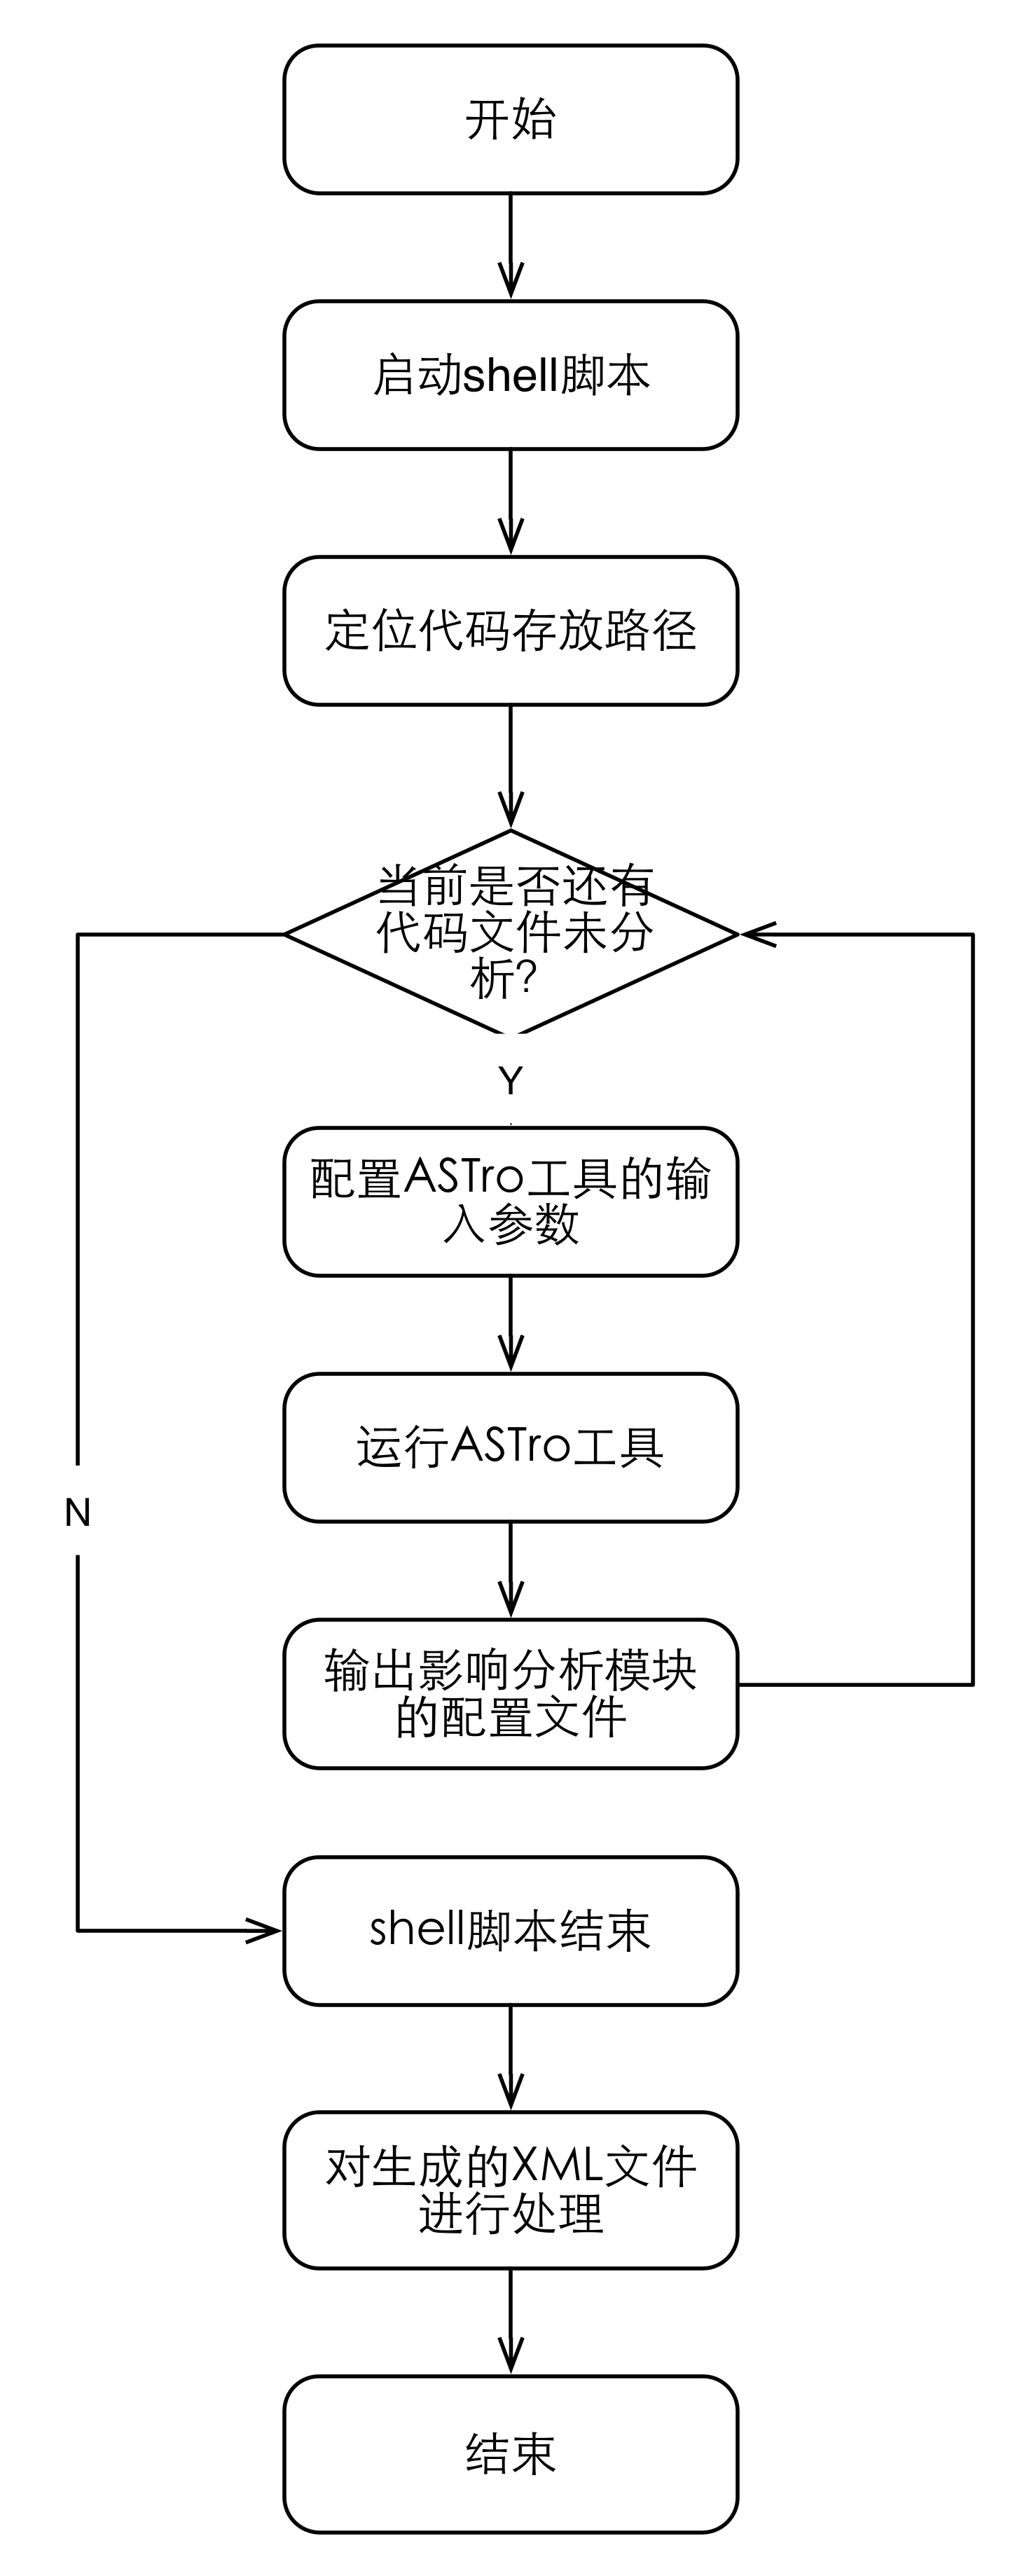
\includegraphics[height=.8\columnwidth]{chap04_differ}
	\caption {程序间差异性分析流程}
	\label {diff}	
\end{figure}



%图中所描述的软件变更集合可以定义如下:
%\begin{definition}
%	$ change\_set = \{ (old_i,new_i) \mid  old_i \subset Structure,new_i \subset Structure, i \subset \mathbb{N} \}$
%\end{definition}



\section{变更语义影响分析}
\label {chap_impact}
如前所述,变更语义影响分析的过程主要用于根据上一步中得到的变更集合,找到受到变更集合的语义影响的其他程序语法结构的集合,也就是所谓的变更影响域。在该过程中,我们主要关注的是语法结构之间在语义上的相互影响。
%程序变更语义影响分析是$impact$函数的具体实现,主要用于获取变更集合对其他程序结构的影响域。影响域所包含的程序结构直接或间接地受到变更集合中的元素影响。

近年来这方面比较成熟的工作也有不少,因而可以直接选择合适的变更语义影响分析算法作其对应工具模块的具体实现。


\subsection{相关定义}

本节中主要介绍与变更语义影响分析相关的概念和定义。以下所指的影响都是语义影响。

\begin{definition}
	$im: \mathcal{S} \mapsto \mathcal{S}$。该函数描述了程序语法结构之间的影响关系,$\forall s_i,s_j \subset \mathcal{S},i,j \subset \mathbb{N}$,如果$im(s_i) = s_j$,则说明语法结构$s_i$受到$s_j$的影响。
\end{definition}

事实上,影响是由于代码之间存在着某种依赖关系而造成的。如果给出不同的依赖关系的定义,那么就会得到不同类型的影响。可见,这里所谓的影响即是程序代码间的耦合关系。常见的依赖关系包括控制依赖和数据依赖等。

有了影响的定义以后,我们就能得到变更影响域的概念。前文中所提到的变更影响域,也就是变更的语义影响域(Sematic Impated Area)是指在程序的某个限定的影响范围中,直接或间接受到变更影响的程序语法结构集合。影响范围实际上描述了变更所造成影响的传播范围。

因此,变更影响域可以较形式化的定义如下:

\begin{definition}
	$impact: \mathcal{P} \times \mathcal{C} \mapsto \{\mathcal{S}\}$。$impact(p,v) = \{s_k\}$,其中$im(s_k)$要么是变更集合$p$中所改变的语法结构,要么是$impact(p,v)$中的已有元素,$p \subset \mathcal{P},v \subset \mathcal{C}, s_k \subset \mathcal{S},k \subset \mathbb{N}$。这里的$s_k$其选取受限于影响范围和语法结构类型的选择。可见,变更影响域描述了变更集合在代码$\mathcal{C}$上所影响到的$\mathcal{S}$的集合。最后得到的$\mathcal{S}$的集合即为直接或间接受到变更影响的语法结构的集合,也就是所谓的变更的语义影响域(即变更影响域)。
\end{definition}

在变更影响域的计算过程中,需要考虑到其计算的精度。考虑到上文中的定义,则该过程的计算精度主要受到影响范围和语法结构类型的影响。根据前文中对于$\mathcal{S}$的定义,可以将程序中受变更影响的语法结构划分为不同的粒度,从而获得不同程度的影响\cite{petrenko2009variable}。而影响范围的粒度则可以划分为:
\begin{enumerate}
	\item 类间:考虑变更的影响可能延伸到其他类(对象)。
	\item 方法间:考虑变更的影响可能延伸到其他方法内部。
	\item 方法内部:考虑变更的影响只在本方法的内部延伸。
\end{enumerate}

显然,不同级别的影响范围会对变更语义影响分析的精度产生显著影响。在实践过程中,不同级别的影响范围均可采用不同的语法结构类型,以获得合适精度的变更影响域。

因此,如前文所述,$impact$函数描述了整个变更语义影响分析的过程,该分析过程需要输入代码$v$和补丁$p$,其计算结果为在$v$中某个范围内受到$p$中变更集合影响的语法结构集合,即变更影响域。

\subsection{分析方法}

在本文的兼容性检测方法中,该分析过程应当接受两个不同版本代码间的变更集合作为输入,并输出变更集合所对应的语义影响域,也就是我们所需要的变更影响域。变更语义影响分析的过程可以通过控制流、数据流等信息分析出变更集合中每条变更对其他程序语法结构是否存在影响,并进行闭包计算。

本文对于该分析过程的要求如下:
\begin{itemize}
	\item 接受两个不同版本代码间的变更集合作为输入。
	\item 计算得到该变更集合所对应的影响域。
	\item 计算过程中可以指定受影响的范围和语法结构类型。用于设置分析的精度。
	\item 具有影响追踪系统,将计算影响域的过程进行记录。方便后续的冲突检测过程回溯影响的来源。
\end{itemize}

%其中影响追踪系统可以定义成如下类型的函数。该函数接受一个影响域分析函数$ia(v_i,v_j)$,并返回对应的依赖关系集合。
%
%\begin{definition}
%	$impact\_track(ia(v_i,v_j)):(Code \times Code \mapsto {Structure}) \mapsto {depend}$
%\end{definition}


%该分析过程如图\ref {impact_analyzer}所述,其中的$impact$函数可以任意选择某一能够满足上述要求的变更语义影响分析算法。
%
%图中所描述的变更影响集合可以定义如下:
%\begin{definition}
%	$impact\_set = \{ (structure_i) \mid  structure_i \subset Structure, i \subset \mathbb{N}\}$
%\end{definition}
%
%\begin{figure}[H]
%	\centering
%	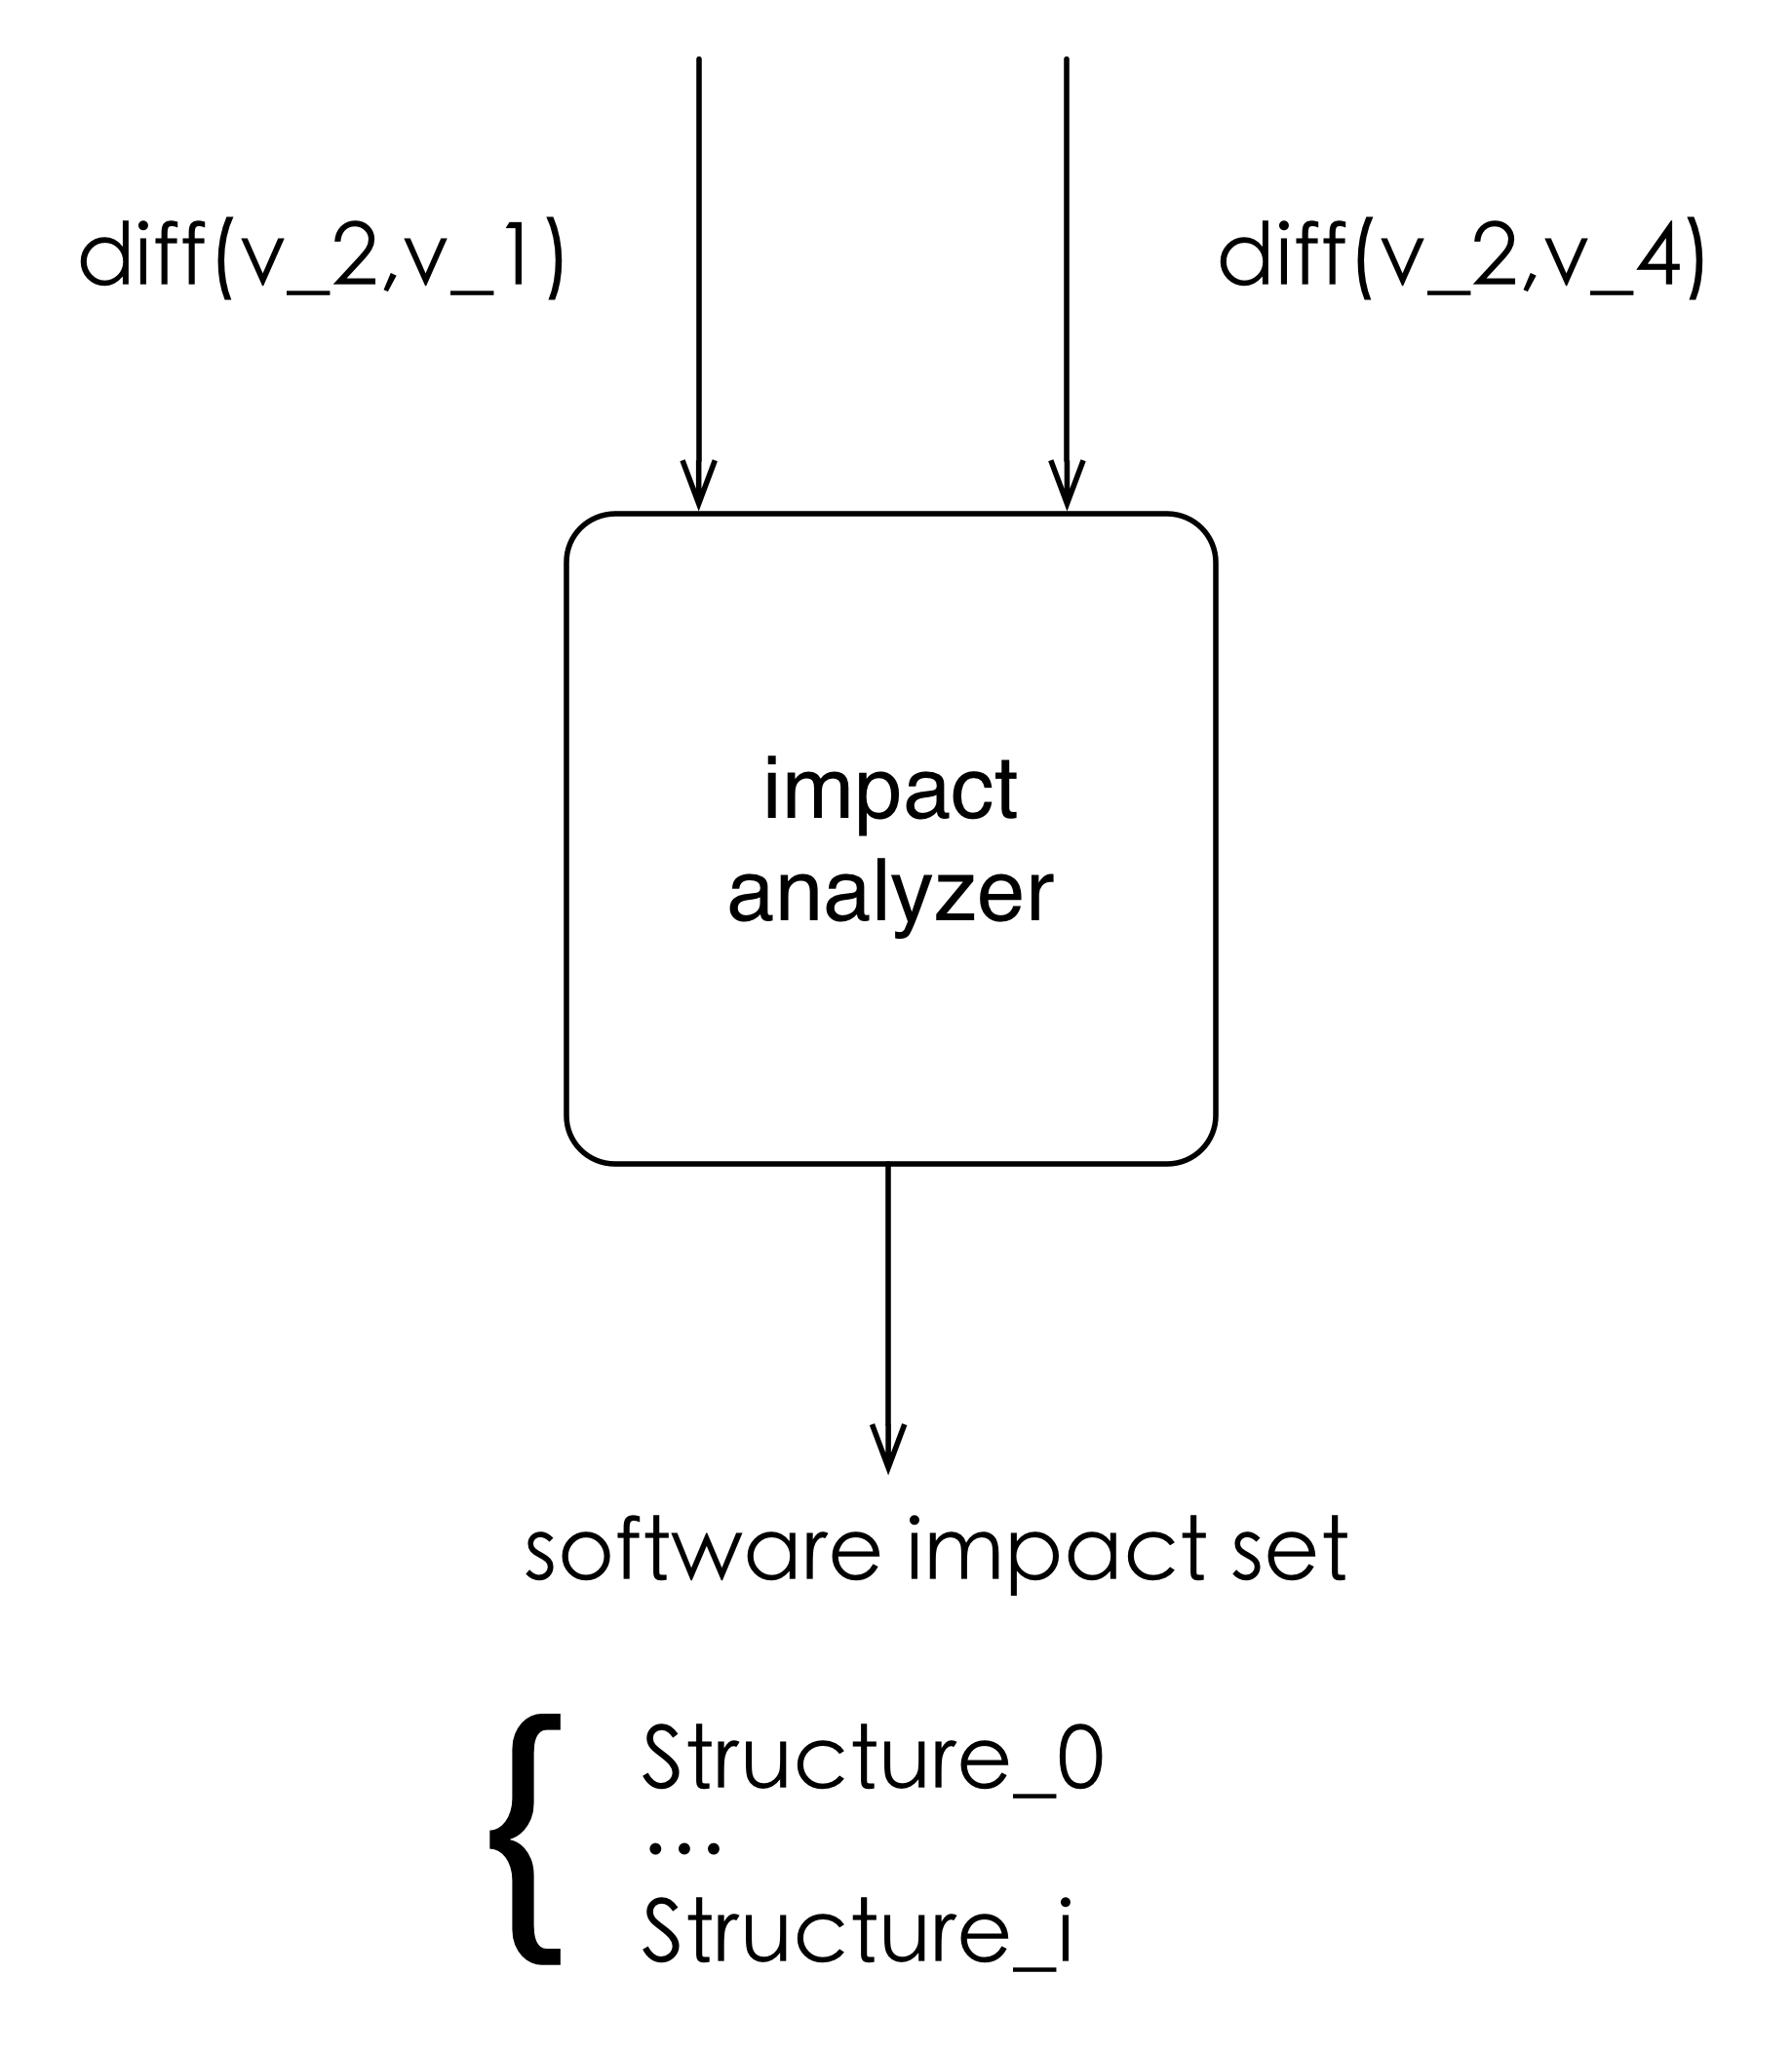
\includegraphics{chap03_impact}
%	\caption {程序间差异分析}
%	\label {impact_analyzer}	
%\end{figure}

\subsection{模块设计与实现}

在实现该模块的过程中,本文主要采用了jpf-regression工具的变更语义影响分析算法。jpf-regerssion是DiSE方法在Java Path Finder软件框架下的具体实现,提供了方法内和方法间的程序语句级别的变更语义影响分析。在实现过程中,我们采用了较为简单的分析精度设置,将影响范围限制在方法内部,将受影响的语法结构类型设置为基本块。

该子模块主要实现了$impact$函数的实际功能,它接受差异性分析模块中输出的变更集合,计算其变更影响域并将其输出。


%\subsubsection{设计}
%
%在该模块的设计中,其输入输出过程可以描述如图\ref {impact},输入输出的具体描述参见表\ref {impact_io}。
%
%考虑到该模块需要的核心任务包括:
%\begin{itemize}
%	\item 变更语义影响分析
%	\item 影响追踪:记录影响分析过程的轨迹,即影响的依赖关系$depend$。
%	\item 输入输出
%\end{itemize}
%
%因此,该模块的设计可以参考图\ref {des_impact}。
%
%该模块的流程也就可以设计成如下的形式:
%\begin{enumerate}
%	\item 读取输入
%	\item 变更语义影响分析,并进行影响追踪
%	\item 结果输出
%\end{enumerate}
%
%\begin{figure}[H]
%	\centering
%	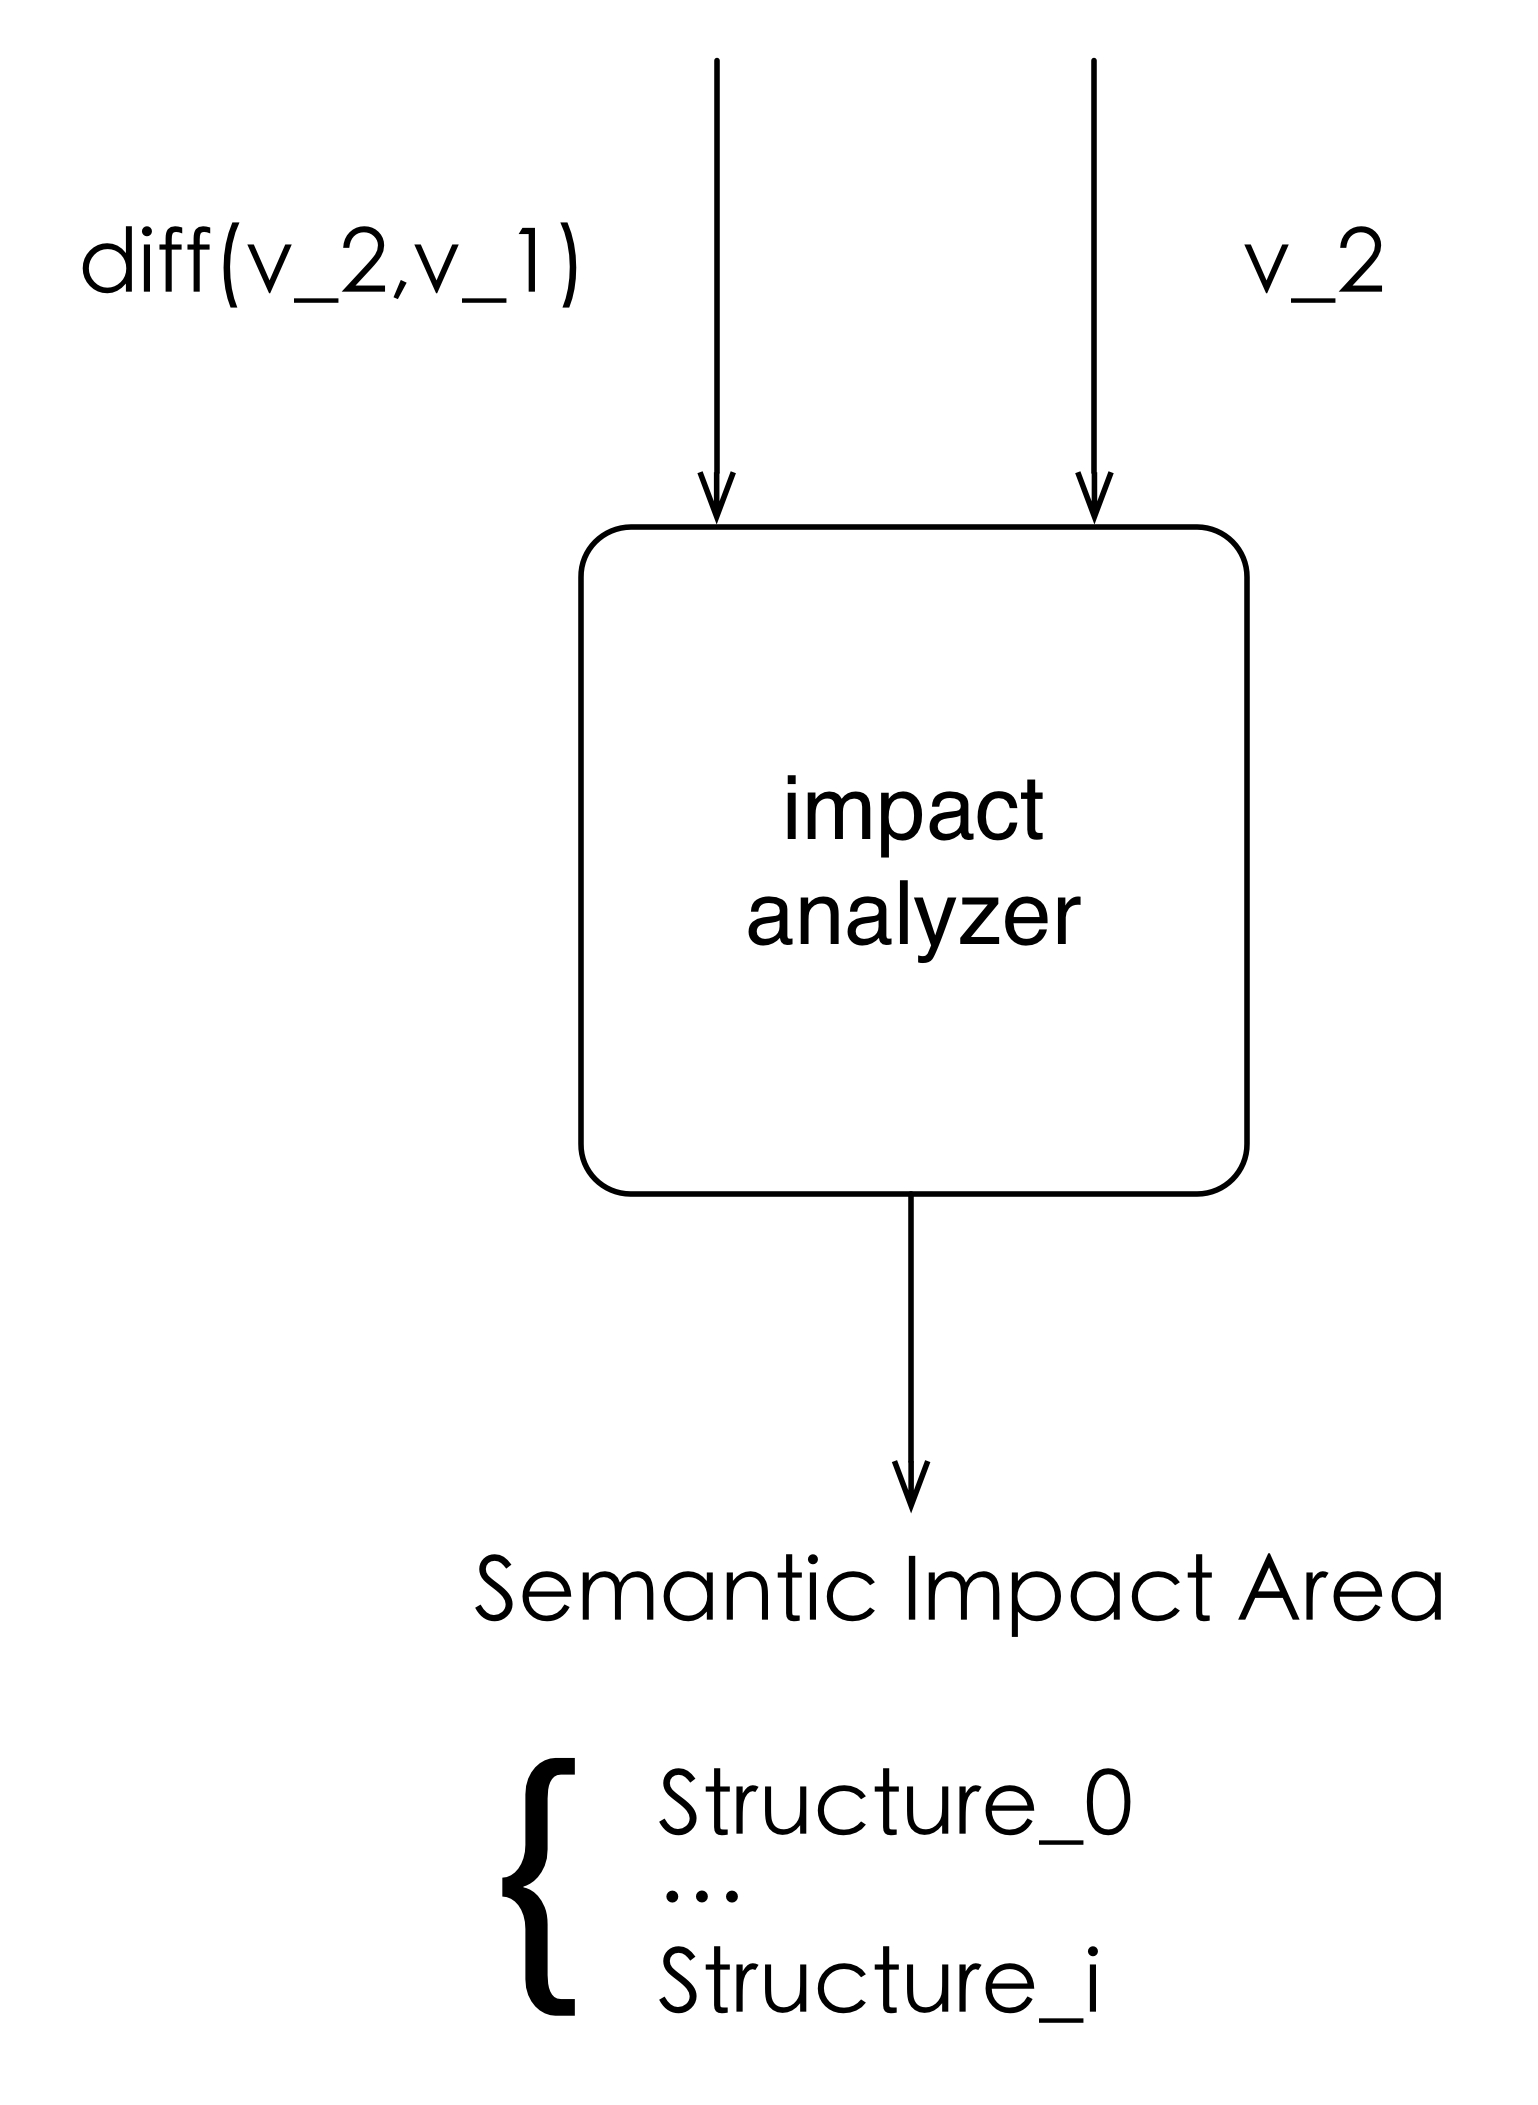
\includegraphics[height=.6\columnwidth]{chap03_impact2}
%	\caption {影响分析模块}
%	\label {impact}	
%\end{figure}
%
%
%\begin{table}[H]
%	\caption{输入输出对照表}
%	\label{impact_io}
%	\centering
%	\begin{tabular}{lc}
%		\toprule[1.5pt]
%		{\heiti 输入输出} & {\heiti 描述} \\\midrule[1pt]
%		$diff(v_2,v_1)$ & 差异性分析模块的输出,变更集合 \\
%		$v_2$ & 源代码 \\
%		语义影响域 & 语义影响域,即$v_2$中受变更影响的代码结构集合\\
%		\bottomrule[1.5pt]
%	\end{tabular}
%\end{table}
%
%\begin{figure}[H]
%	\centering
%	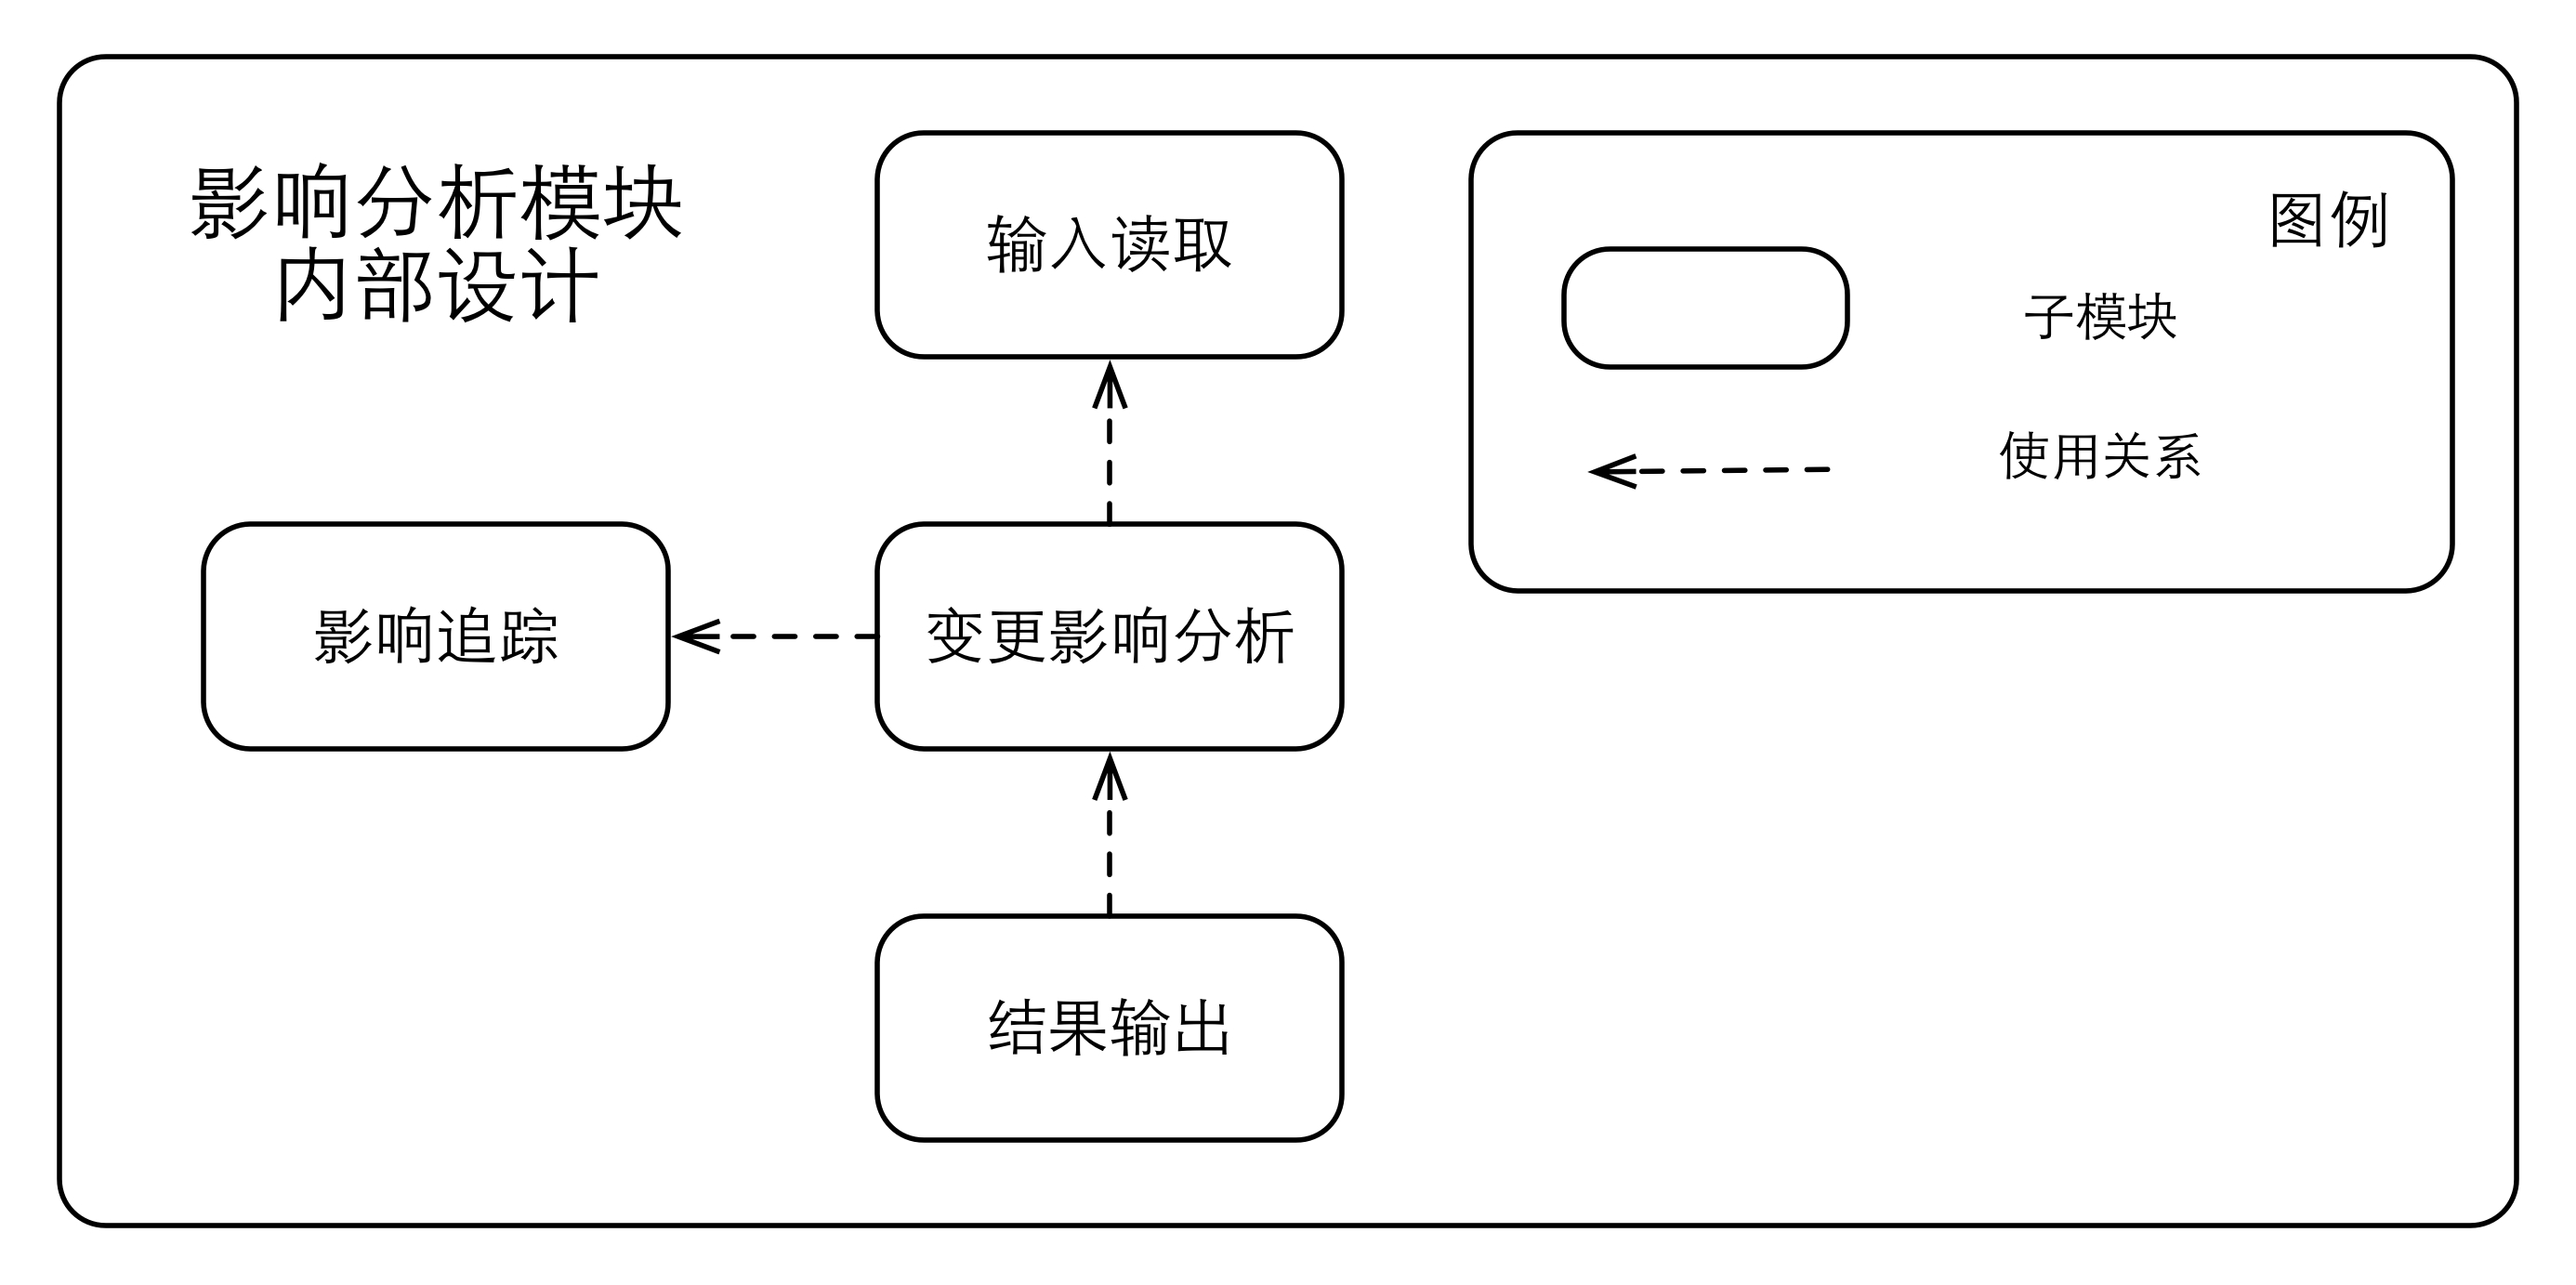
\includegraphics[width=.8\columnwidth]{chap04_impact_internal}
%	\caption {模块设计}
%	\label {des_impact}	
%\end{figure}
%
%\subsubsection{实现}


在使用过程中,jpf-regression工具接受Java格式的源代码和ASTro提供的变更集合作为输入,并输出影响域信息至Dot文件中。

Dot是一种采用文本进行描述的图形格式,以该格式输出的实际上是整个源代码的控制流图(Control Flow Graph),而变更影响域作为该控制流图额外承载的信息,在CFG上进行了标注。可见,该模块实际上将影响域信息输出为图形表示。

因此,该模块中输出的影响域的相关信息主要包括两类:
\begin{itemize}
	\item 受影响的CFG节点。这实际上就是影响域中的元素。可见这里受影响语法结构的级别为基本块。
	\item 节点间的影响关系。这实际上是记录了影响关系的来源,即控制依赖、数据依赖等。
\end{itemize}

%该模块的实际输入输出可以参考表\ref {impact_io2}。
%
%\begin{table}[H]
%	\caption{输入输出对照表}
%	\label{impact_io2}
%	\centering
%	\begin{tabular}{llc}
%		\toprule[1.5pt]
%		{\heiti 输入输出} & {\heiti 描述} & {\heiti 格式} \\\midrule[1pt]
%		输入 & 差异性分析模块的输出,变更集合 & XML \\
%		输入 & 源代码 & Java \\
%		输入 & 源代码 & Class \\
%		输入 & 配置文件 & JPF \\
%		输出 & 语义影响域+控制流图 & Dot \\
%		\bottomrule[1.5pt]
%	\end{tabular}
%\end{table}



然而jpf-regression工具中变更语义影响分析只是其中的一个子模块,主要用于为其后续的DiSE分析过程服务。因而在实践过程中,我们可以重用jpf-regression的代码,并对其加以改造,使其符合本文的实际需要。主要的变化包括:
\begin{enumerate}
	\item 修改分析流程。
	\item 增加影响追踪系统。
	\item 增加错误记录系统。
	\item 使其适应大规模批量化分析的需要。
	\item 已知Bug修复。
\end{enumerate}

下面分别进行介绍。

jpf-regression作为Java Path Finder框架的一个插件,事实上在使用时需要遵守该框架的约束,有明确的执行流程规定。然而在实际使用中,该流程约定与我们的实际情况并不符合,因而我们对此进行了一定的修正。

事实上,原执行流程约定,每次分析以源代码文件中的Main函数作为入口,探索并分析Main函数所调用的其他函数。该流程对于大部分情况而言是具有实际意义的,并且由于只考虑Main函数及其调用的函数,工具可以节约分析的开销,更快的得出结论,而忽略掉其他事实上并未在执行过程中被涉及到的函数。

然而对于我们的分析需要而言,该流程只能覆盖到部分情况,对于其他类型的软件系统而言可能并不适用,例如以Eclipse JDT Core项目而言,该项目主要用于为Eclipse软件系统的其他组件提供服务,因而在实际中以JAR包的形式作为库函数而存在。对于这类以库函数形式对外提供服务的源代码而言,他们并不存在入口函数,也无法预知到底会有哪些函数会被外界所调用。因而对于这类情况而言,我们需要在分析过程中覆盖其所有函数,以保证结果的完整性和正确性。

我们对于流程的修改可以参考图\ref {impact_process_old}进行对比。首先我们去掉了图\ref {impact_process}中所示的JPF框架启动流程,直接调用jpf-regression的核心功能。其次,如图\ref {impact_process_old}所示,我们将待计算的方法集合从Main函数的调用函数集合修改为文件中所有方法的集合,并在相应的影响集合计算过程中增加了影响追踪系统。

\begin{figure}[H]
	\centering
	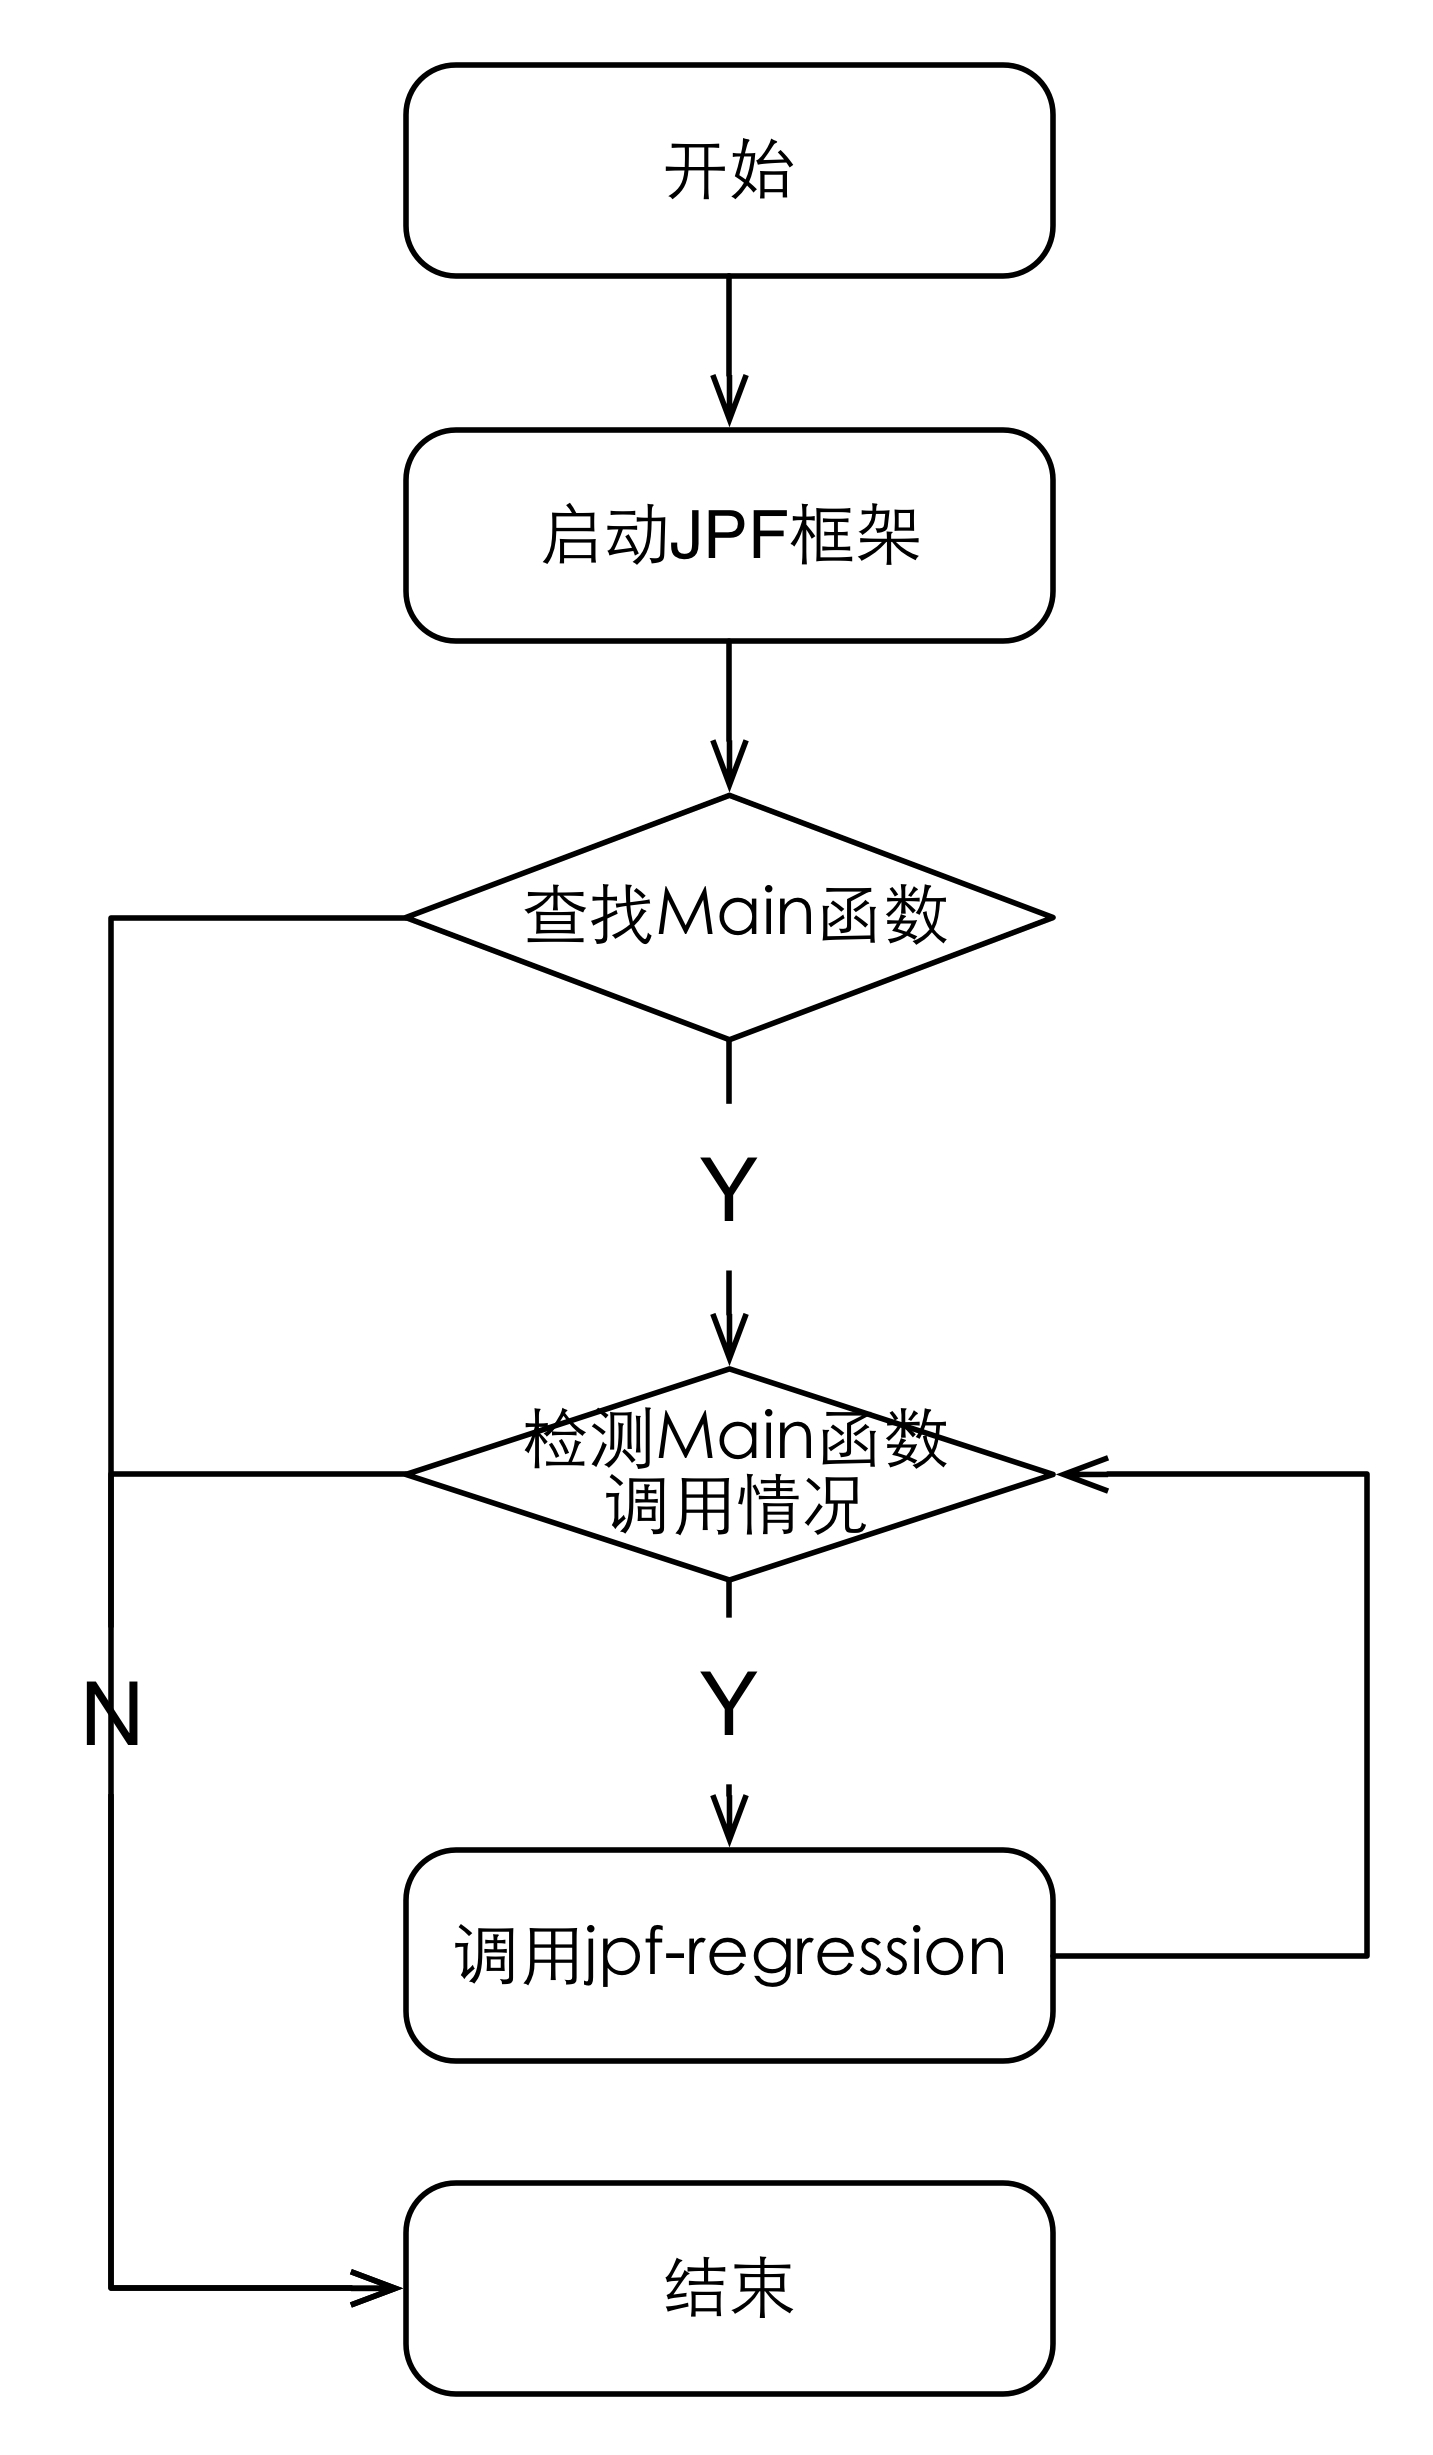
\includegraphics[height=.8\columnwidth]{chap04_jpf_launch}
	\caption {jpf框架启动流程}
	\label {impact_process}	
\end{figure}


\begin{figure}
	\centering
	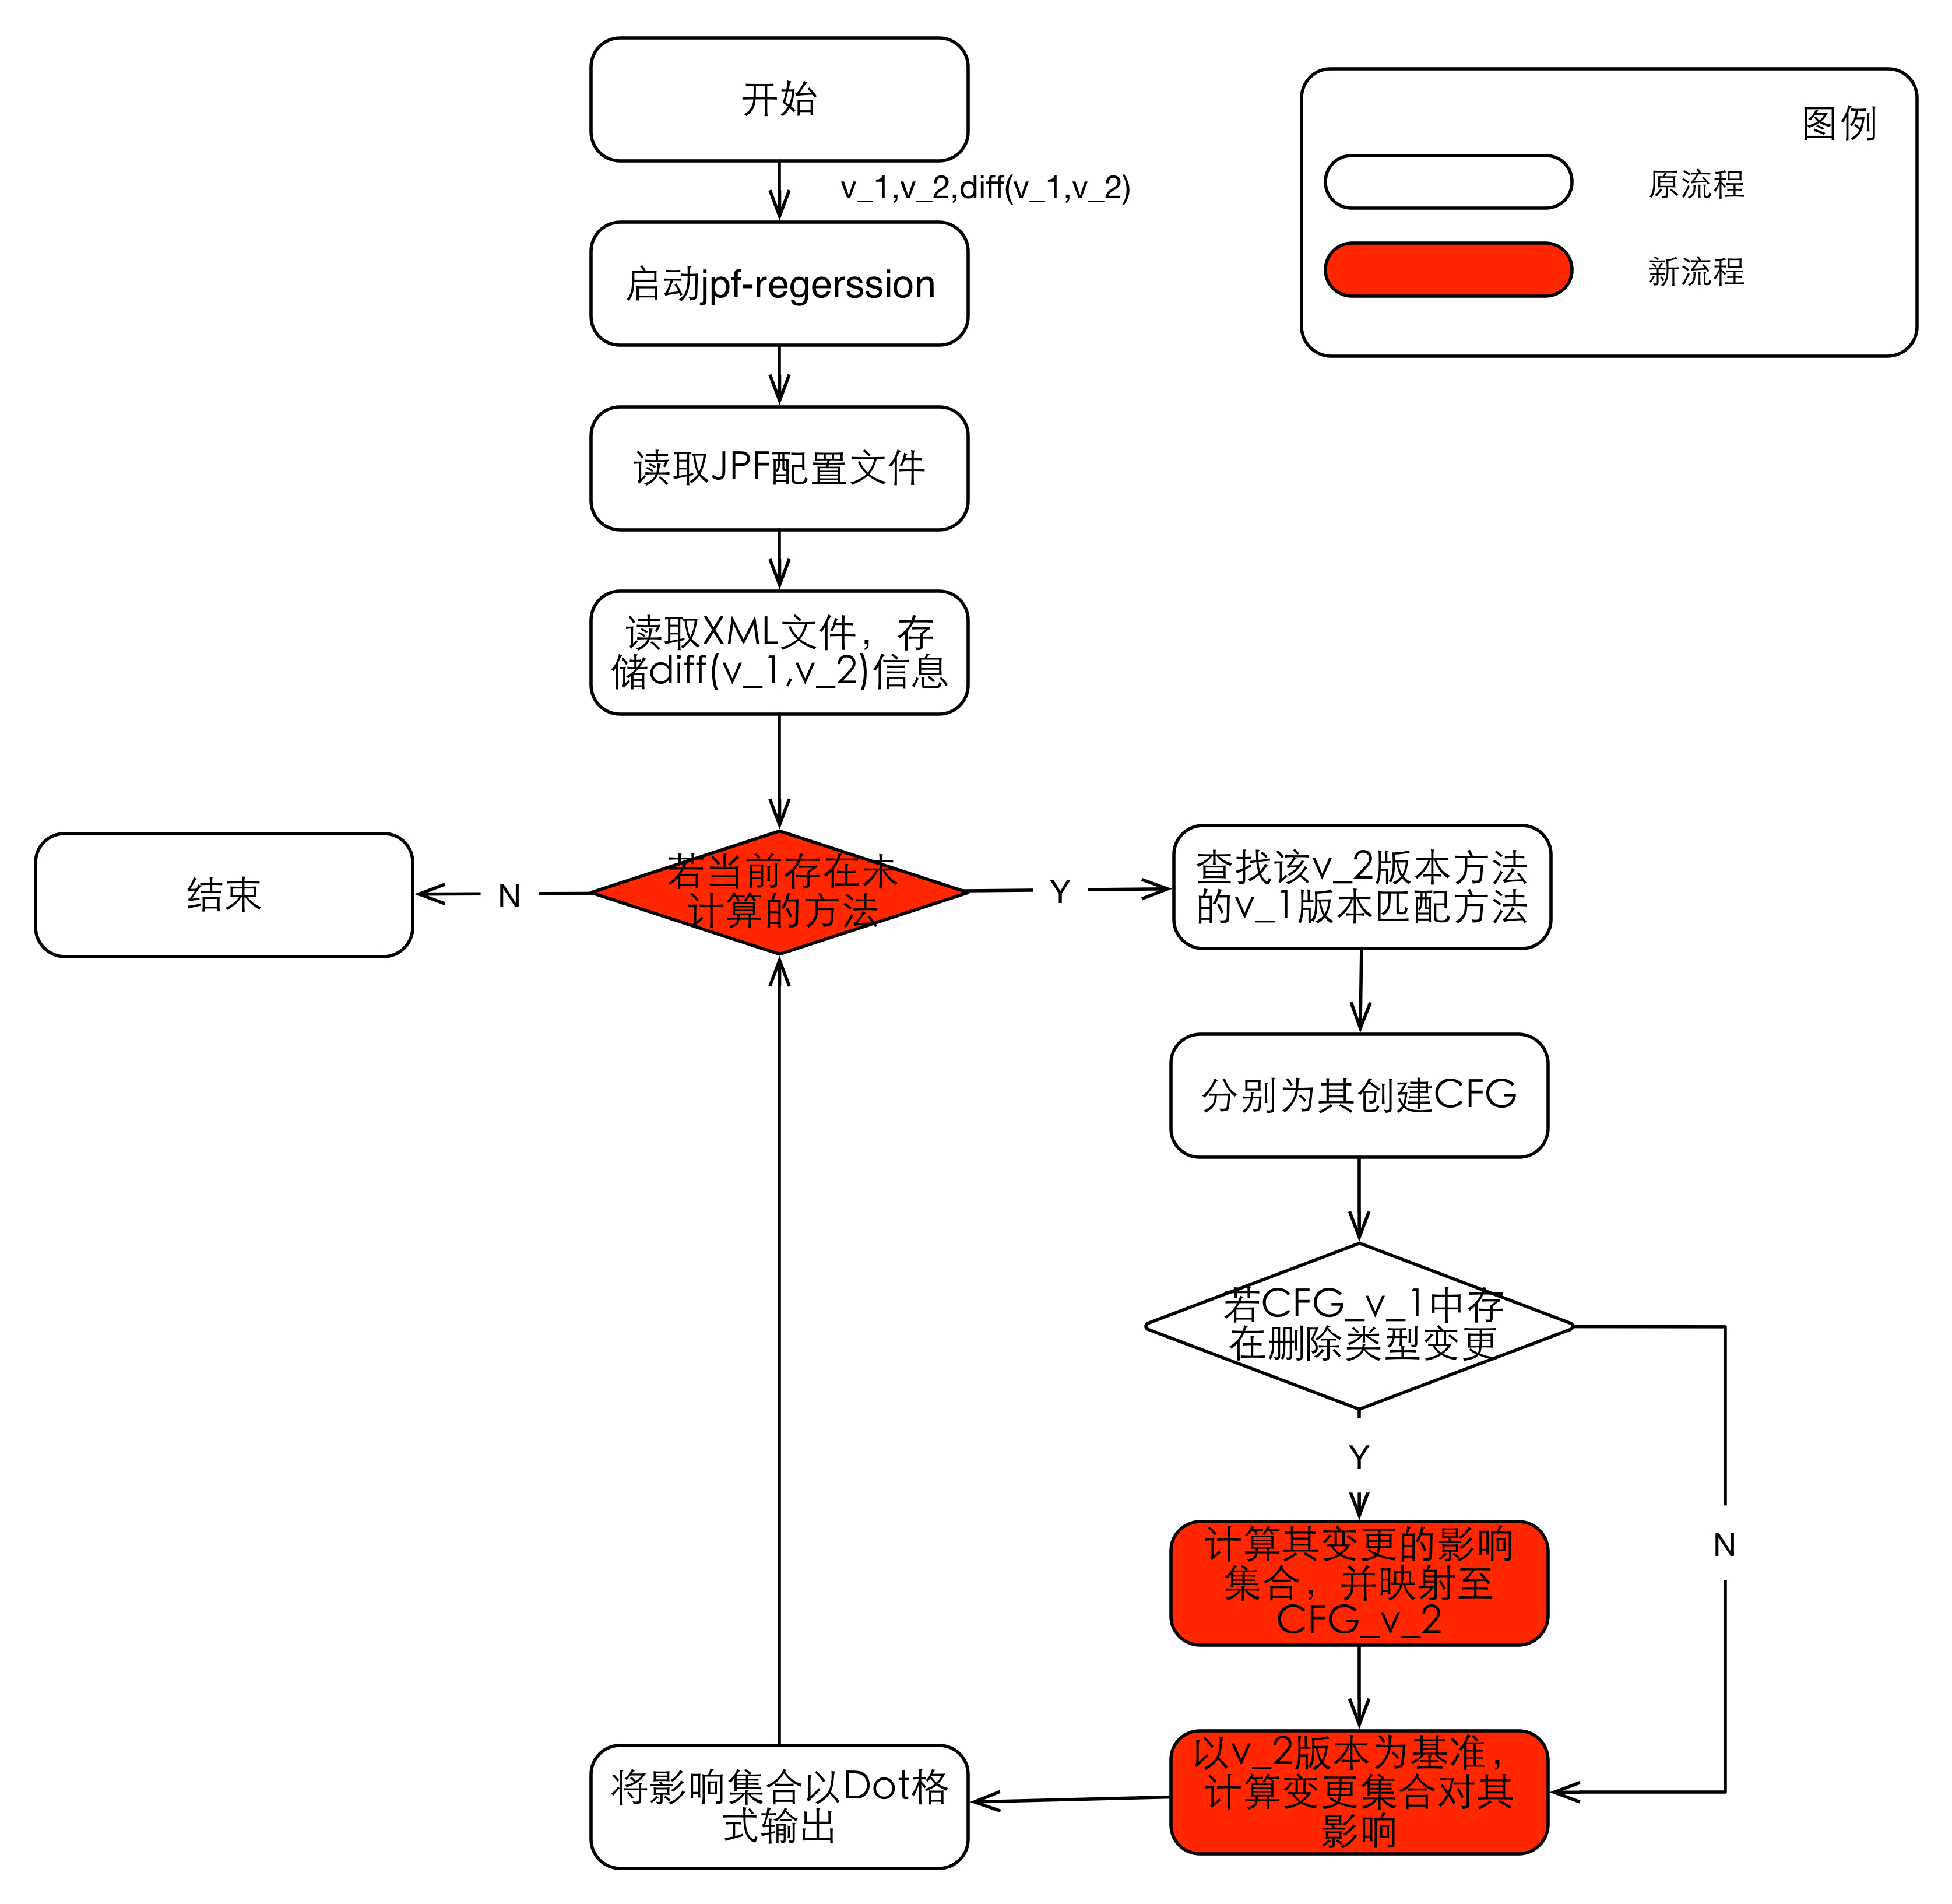
\includegraphics[width=.8\columnwidth]{chap04_jpf_old}
	\caption {jpf-regression原流程及变化}
	\label {impact_process_old}	
\end{figure}



在后续的冲突判定过程中,对于找到的可能发生冲突的位置,我们需要对其追根溯源,挖掘其影响来源,以进行人工分析,判定该情况是否确实冲突。因此,我们需要在变更语义影响分析的阶段加入影响追踪系统,以便记录下变更影响的轨迹,根据这些信息为后续的分析过程提供便利。

为了实现影响追踪系统,我们需要存储程序结构间的影响关系。如前所述,影响的来源主要有两类,即:
\begin{itemize}
	\item 控制依赖
	\item 数据依赖
\end{itemize}

因而,为了描述该影响关系,本文设计了Dependency类族,参见图\ref {class_depend}。该类中使用了一个二元组的数据结构depend来存储影响来源和受影响对象,并使用了多态机制来区分影响关系的类型,即是控制依赖还是数据依赖。Dependency类族中重写了hashCode()方法和equals()方法,以便能够放入集合中进行存储。

影响追踪系统中具体使用到的数据结构可以参考表\ref {track_data}。

\begin{figure}[H]
	\centering
	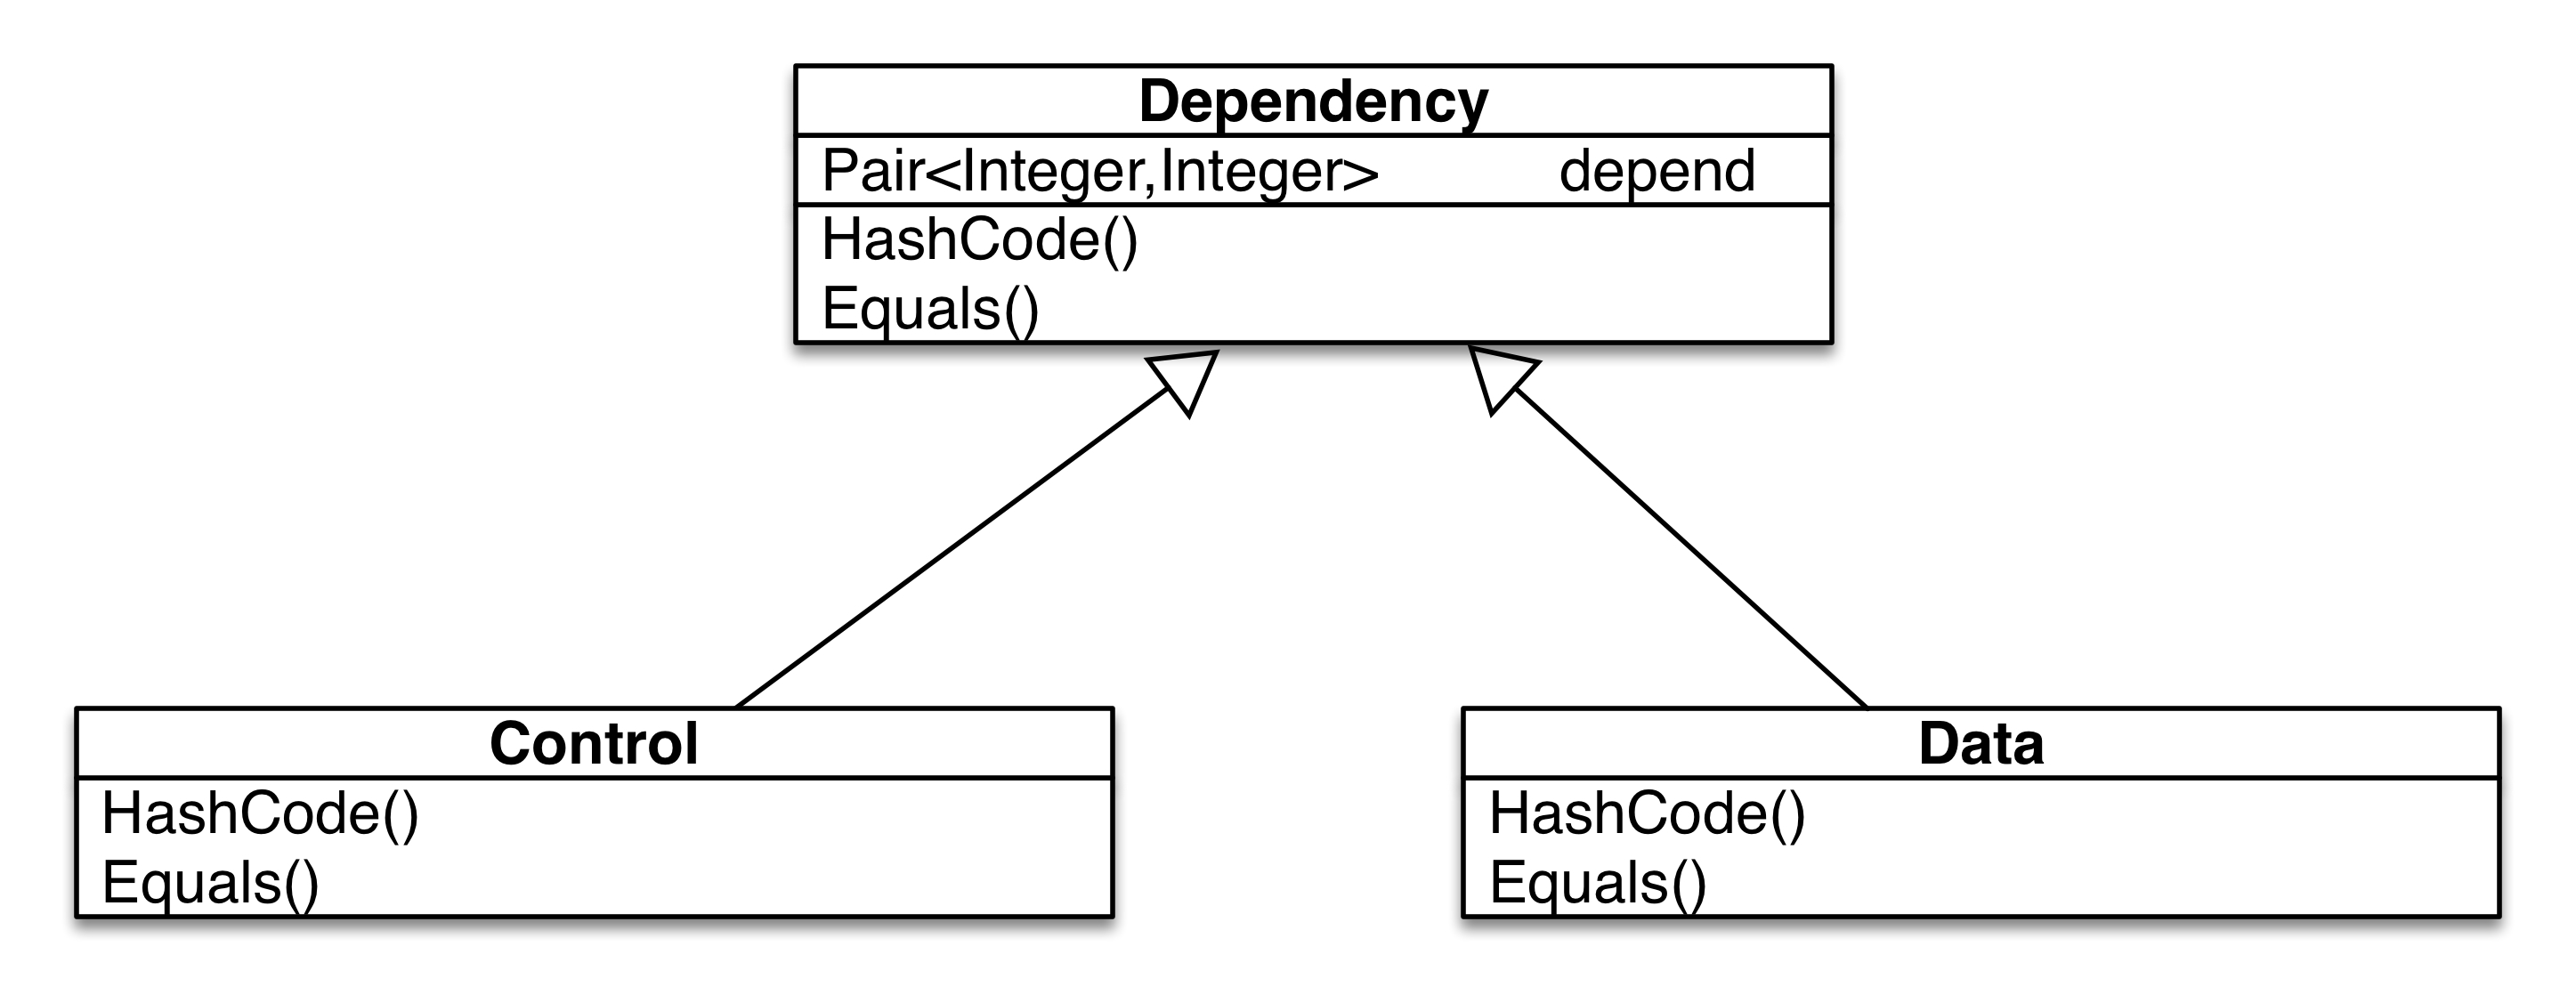
\includegraphics[width=.8\columnwidth]{chap04_depend}
	\caption {Dependency类族}
	\label {class_depend}	
\end{figure}

\begin{table}
	\caption{影响关系数据结构}
	\label{track_data}
	\centering
	\begin{tabular}{lllc}
		\toprule[1.5pt]
		{\heiti 数据类型} &{\heiti 数据结构} & {\heiti 用途} \\\midrule[1pt]
		Dependency & dependency & 单个影响关系 \\
		Control & dependency & 单个控制依赖影响关系 \\
		Data & dependency & 单个数据依赖影响关系 \\
		Map<Integer, Set<Dependency> > & depend & 存储计算过程中的全部影响关系\\
		\bottomrule[1.5pt]
	\end{tabular}
\end{table}

影响关系的创建需要在进行变更语义影响分析过程的同时进行,以便记录下所有的依赖。最后将其作为影响域相关信息的一部分进行输出。在实现过程中,将其作为控制流承载的额外信息即可。

原有的jpf-regression工具由于是单次分析过程,因而一旦在运行过程中遇到问题,就会采用抛出异常终止运行的方式结束分析。然而我们在实际情况中需要进行大规模的分析作业,如果仅仅在其中单个文件的分析过程中出错就终止整个分析作业,会造成极大的时间和计算资源的浪费。

因而我们对该工具的异常处理方式进行了修改,使其在单次分析过程中如果遇到问题,则会及时抛出异常,但并不终止整个程序的运行,而采取了继续往下执行并分析其他文件的策略。然而分析错误是确实存在的,为了不丢失这类错误信息,我们为工具添加了错误记录系统,不断记录单次分析过程中遇到的问题。

我们对程序运行过程中可能出现的报错情况进行了分类,并设计了专门的错误统计类以专门别类的对错误情况进行记录和统计。该类的设计可以参考图\ref {class_error}。其中使用到的数据结构可以参考表\ref {error_data}的说明。

\begin{figure}[H]
	\centering
	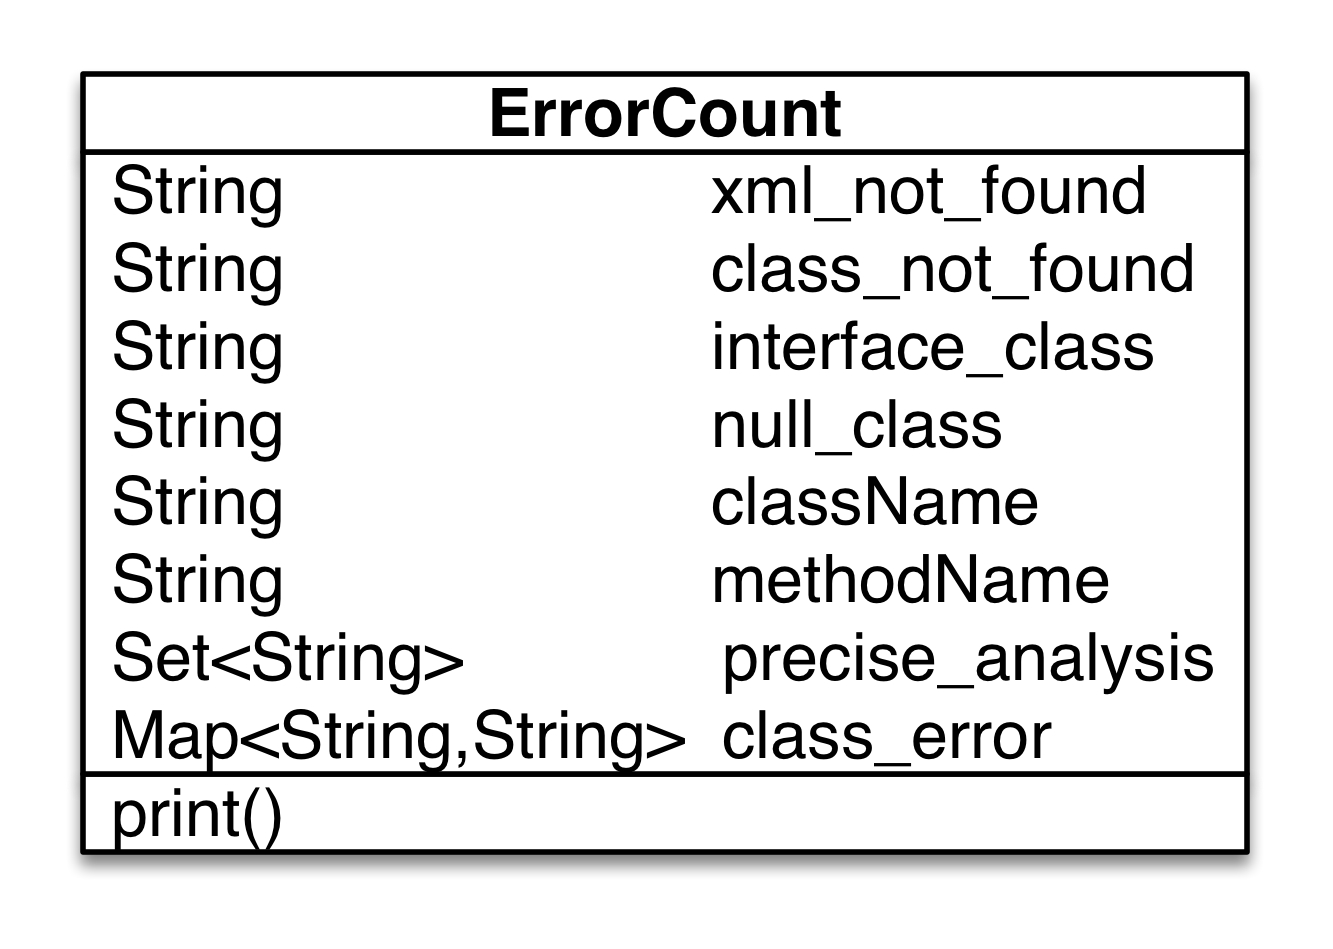
\includegraphics[width=.8\columnwidth]{chap04_error}
	\caption {ErrorCount类}
	\label {class_error}	
\end{figure}

\begin{table}
	\caption{错误记录数据结构}
	\label{error_data}
	\centering
	\begin{tabular}{lllc}
		\toprule[1.5pt]
		{\heiti 数据类型} &{\heiti 数据结构} & {\heiti 用途} \\\midrule[1pt]
		String & xml\_not\_found & 错误:XML文件未找到 \\
		String & class\_not\_found & 错误:Class文件未找到 \\
		String & interface\_class &  错误:接口类\\
		String & null\_class & 错误:类中无具体实现(如抽象类)\\
		Set<String> & precise\_analysis & 记录有多少方法在影响计算过程中出错\\
		Map<String, String> & class\_error & 记录有哪些类出现了哪些错误\\
		void & print() & 输出错误记录\\
		\bottomrule[1.5pt]
	\end{tabular}
\end{table}


原有的jpf-regression工具只能支持单次分析过程,在实际情况中我们需要工具具备大规模批量化分析的能力,以应对大规模软件系统的实际需求。为此我们可以保留原有的单次分析过程,然后在其上层进行封装,循环多次调用单次分析过程,以达到批量化自动分析的效果。这个过程由于进行了封装,对于用户而言是透明的。

同时,在进行大规模分析的时候,输出文件的命名格式也需要修改。在原单次分析过程中,输出文件直接采用被分析的方法名进行命名。对于分析小型文件而言,这种设计就足够了,然而在大规模分析的时候,我们需要进行一定的优化。

由于大规模分析时,可能存在一些现象,例如:
\begin{enumerate}
	\item 函数重载
	\item 不同版本间的代码其方法可能无法一一匹配。例如有的方法仅在单个版本的代码中出现。
\end{enumerate}

这些现象会使得工具中原有的输出文件命名方式不太合用。在这种情况下,我们采用的新命名格式为:

$MethodName+HashCode(MethodName)+ExtensionName$

其中,$MethodName$由即为方法名,无法保证方法名的唯一性。再利用Java中的HashCode方法,对$MethodName$计算其HashCode作为其后缀,以保证方法名的唯一性。最后$ExtentionName$即为文件扩展名,在jpf-regression中$ExtentionName = “.dot”$。

同时我们也保留了原有的单次分析能力,以满足实际情况中的其他需要,例如进行小规模的案例分析。

最后,在进行大规模分析的情况下,由于实验数据量的庞大,我们无法按照单次分析过程中那样去人工查看并分析实验结果。因此,为了适应这种需要,我们还增加了数据统计模块,使得程序具备一定的自动化分析实验结果的能力。

大规模分析的相关类实现可以参考图\ref {class_run_all}和图\ref {class_run_jpf}。其中涉及的数据结构及其说明参考表\ref {run_all_data}和表\ref {run_jpf_data}。在实现中,RunAll会读取所有待分析的文件名并找到其配置文件地址,然后循环调用Runjpf对象进行单次分析过程。

\begin{figure}[H]
	\centering
	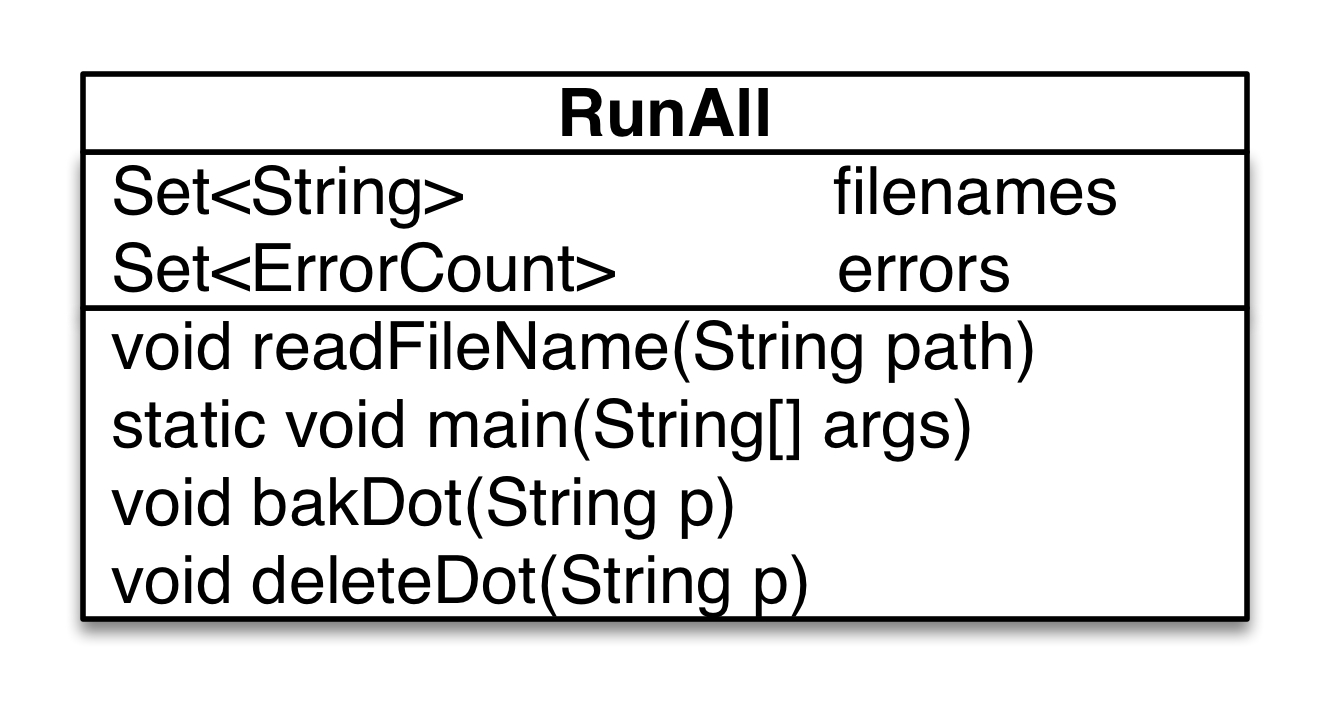
\includegraphics[width=.8\columnwidth]{chap04_run_all}
	\caption {RunAll类}
	\label {class_run_all}	
\end{figure}

\begin{figure}[H]
	\centering
	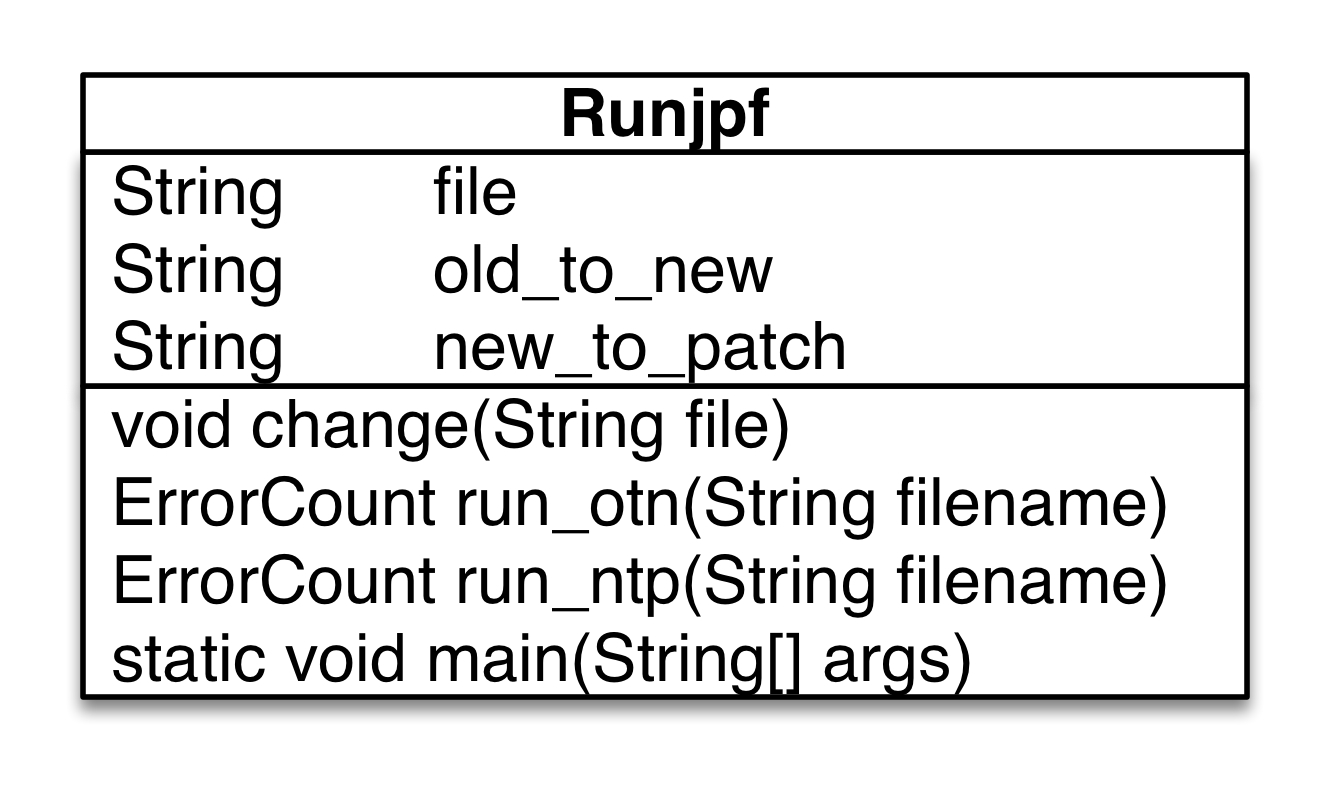
\includegraphics[width=.8\columnwidth]{chap04_run_jpf}
	\caption {Runjpf类}
	\label {class_run_jpf}	
\end{figure}

\begin{table}
	\caption{RunAll数据结构}
	\label{run_all_data}
	\centering
	\begin{tabular}{lllc}
		\toprule[1.5pt]
		{\heiti 数据类型} &{\heiti 数据结构} & {\heiti 用途} \\\midrule[1pt]
		Set<String> & filenames & 存储待分析的文件名 \\
		Set<ErrorCount> & errors & 存储每次分析中出现的错误 \\
		void & readFileName(String path) & 从文件中读取待分析的文件名\\
		static void & main(String[] args) & 实现大规模分析过程\\
		void & bakDot(String p) & 备份分析结果\\
		void & deleteDot(String p) & 删除分析结果\\
		\bottomrule[1.5pt]
	\end{tabular}
\end{table}

\begin{table}
	\caption{Runjpf数据结构}
	\label{run_jpf_data}
	\centering
	\begin{tabular}{lllc}
		\toprule[1.5pt]
		{\heiti 数据类型} &{\heiti 数据结构} & {\heiti 用途} \\\midrule[1pt]
		String & file & 待分析文件名\\
		String & old\_to\_new & $impact(diff(v_2,v_1),v_2)$过程的配置文件位置\\
		String & new\_to\_patch & $impact(diff(v_2,v_4),v_2)$过程的配置文件位置\\
		void & change(String file) & 改变当前需要读取的配置文件\\
		ErrorCount & run\_otn(String filename) & 运行$impact(diff(v_2,v_1),v_2)$过程 \\
		ErrorCount & run\_ntp(String filename) & 运行$impact(diff(v_2,v_4),v_2)$过程  \\
		static void & main(String[] args) & 实现单次分析过程\\
		\bottomrule[1.5pt]
	\end{tabular}
\end{table}


在实际使用jpf-regression进行实验的过程中,我们发现该工具存在一些Bug,这些Bug或多或少的导致了分析结果的正确性和精度降低。我们对其中力所能及的Bug进行了修复,并对这些Bug进行了总结。

目前已知的Bug及其修复情况可以参见表\ref {bug_data}。

\begin{table}
	\caption{Bug报告}
	\label{bug_data}
	\centering
	\begin{tabular}{lllc}
		\toprule[1.5pt]
		{\heiti Bug} &{\heiti 危害} & {\heiti 修复} \\\midrule[1pt]
		内部类无法进行方法匹配 & 小 & 否\\
		只有只有单个版本代码中存在某个方法时无法进行方法匹配 & 小 & 是\\
		将$CFG_{v\_1}$的影响集合映射到$CFG_{v\_2}$时判断条件出错 & 大 & 是\\
		依赖JAR包jpf\_guided\_test出错 & 小 & 否\\
		依赖JAR包jpf\_symboc出错 & 小 & 否\\
		\bottomrule[1.5pt]
	\end{tabular}
\end{table}

\section{本章小结}

本章中主要介绍了软件变更影响域分析方法和其对应的模块设计与实现过程。
章节\ref {chap_diff}中介绍了程序间差异性分析方法和其对应的模块设计与实现。
章节\ref {chap_impact}中介绍了变更语义影响分析方法和其对应的模块设计与实现。

\chapter{实验}
以Eclipse jdt core为例,进行实验,并分析得到的实验结果。
\section{补丁版本迁移}
\section{语义影响范围分析}
\subsection{程序间差异性分析}
\subsection{变更影响分析}
\section{兼容性分析}
\section{结论}
\chapter{结论}
\section{工作总结}

首先,本文提出了软件补丁兼容性检测的问题,并给出了详细的形式化定义。

为了解决这样一个问题,本文通过对该问题进行深入的分析和讨论,提出了一套通用的补丁兼容性分析解决方案,包括以下部分:
\begin{itemize}
	\item 补丁应用
	\item 语义影响域分析
	\begin{itemize}
		\item 程序间差异性分析
		\item 变更影响分析
	\end{itemize}
	\item 冲突分析
\end{itemize}

其中补丁应用过程中的$merge$函数和语义影响域分析的两个子过程$diff$函数和$impact$函数可以自由使用符合要求的相应算法实现,以提高解决方案的实用性。

目前冲突分析过程提出了一种较简单的自动冲突分析算法作为$conflict$函数的实现,更精确的分析结果目前需要人工分析的辅助,为此解决方案中需要变更影响分析过程提供影响追踪函数$impact_track$来追溯语义影响的来源。

其次,本文对该套解决方案采用已有工具给出了具体的工具设计和实现方案,并对该套兼容性检测工具在Eclipse JDT Core项目上进行了测试,发现该工具是确实可用而有效的。它切实能够挖掘出补丁间的语义冲突并向用户进行报告。

可见,本文的主要成果包括:
\begin{itemize}
	\item 提出了软件补丁兼容性检测的问题。
	\item 提出了一套补丁兼容性分析的通用解决方案。
	\item 将解决方案实例化,给出了具体的工具设计与实现方案,并对中型项目Eclipse JDT Core的八个不同版本实施,论证了该解决方案对工业界实际项目的可用性。
\end{itemize}

\section{未来工作}

对于本文中所提到的补丁兼容性解决方案和其工具实现,其可能的未来工作方向包括:
\begin{itemize}
	\item 更换兼容性检测工具中影响域分析模块所使用的工具进行进一步的实验,论证该解决方案的普遍适用性,并讨论兼容性分析的精度与所采用的工具之间的关系。
	\item 将该套工具对更大型的项目进行实验。
\end{itemize}

%%% 其它部分
\backmatter


% 参考文献
\bibliographystyle{thubib}
\bibliography{ref/refs}


% 致谢
\begin{ack}
  感谢贺飞老师对我的悉心指导,他不仅对我的毕设工作和毕业论文的写作给出了许多宝贵的意见,其言传身教更是令我受益匪浅。
  
  其次要感谢实验室的同学和师兄等的帮助,如郭心睿、刘盛鹏、周旻等,他们对我提供了很多帮助,让我铭感于心。
  
  最后要感谢\thuthesis,帮助我顺利完成了本文的写作。
\end{ack}

% 附录
\begin{appendix}
	\input{data/appendix01}
\end{appendix}

% 个人简历
\begin{resume}

  \resumeitem{个人简历}

  1990 年 04 月 03 日出生于 四川 省 绵阳 市。
  
  2008 年 9 月考入 北京理工 大学 软件学院 软件工程 专业,2012 年 7 月本科毕业并获得 工学 学士学位。
  
  2012 年 9 月进入 清华 大学 软件学院 攻读 工程硕士 学位至今。


\end{resume}

\end{document}